\documentclass{scrbook}
\KOMAoptions{paper=a4, fontsize=12pt, chapterprefix=true, twoside=semi, DIV=classic, parskip=half}

\usepackage[T1]{fontenc}
\usepackage[sf]{noto}
\linespread{1.25}

\usepackage{scrlayer-scrpage}
\usepackage[fulladjust]{marginnote}
\usepackage{enumitem}

\KOMAoptions{headsepline=on, captions=besidetop, DIV=last}

\pagestyle{scrheadings}
\automark[section]{chapter}
\setkomafont{pagehead}{\color{RoyalBlue}\slshape\bfseries}
\renewcommand*{\chaptermarkformat}{\chapapp~\thechapter\autodot~--~}
\ofoot*{}
\cfoot*{\pagemark}

\addtokomafont{chapterprefix}{\itshape\color{white}}
\renewcommand*{\chapterformat}{\raggedleft\colorbox{RoyalBlue}{\parbox[b][2.8em]{2.8em}{\vfill\centering{\large\chapapp}\\[-0.4em]\thechapter\vfill}}}
\renewcommand*{\chapterheadstartvskip}{\addvspace{2em}}
\renewcommand*{\chapterheadendvskip}{\pgfornament[width=\textwidth]{88}\par}

\renewcommand*{\sectionformat}{\colorbox{black}{\textcolor{white}{\thesection}}\enskip}
\renewcommand*{\sectionlinesformat}[4]{\makebox[0pt][l]{\rule[-\fboxsep]{\textwidth}{1pt}}#3\parbox[b]{0.85\textwidth}{\linespread{1}\selectfont#4}}

\usepackage{graphicx}
\usepackage[svgnames, dvipsnames]{xcolor}
\usepackage[many]{tcolorbox}
\usepackage{pgfornament}
\usepackage{amsmath,amssymb,amsthm}
\usepackage{bm}
\usepackage{physics}
\usepackage{siunitx}
\usepackage{mathtools}
\usepackage{mdframed}
\usepackage{lipsum}
\usepackage{microtype}
\usepackage{tabularx}
\usepackage{adjustbox}
\usepackage{subcaption}
\usepackage{parcolumns}
\usepackage{multicol}
\usepackage{ifthen}
\usepackage{pgfmath}
\usepackage{pgffor}

\definecolor{mint}{rgb}{0.24, 0.71, 0.54}

\usepackage[lastexercise,answerdelayed]{exercise}
\renewcounter{Exercise}[chapter]
\renewcommand*{\theExercise}{\thechapter.\arabic{Exercise}}
\renewcommand*{\ExerciseHeader}{\textbf{\theExercise )}}
\renewcommand*{\AnswerHeader}{\noindent \textbf{\theExercise}}
\renewcommand*{\ExerciseSkipBefore}{\dimexpr.5\baselineskip}
\renewcommand*{\ExerciseSkipAfter}{\dimexpr.5\baselineskip}

\newtcolorbox{exercisebox}[1][]{
  colback=Mahogany!20, 
  colbacktitle=Mahogany!10,
  coltitle=black,
  colframe=Mahogany,
  fonttitle=\bfseries,
  title=Exercise(s),
  boxrule=0pt,
  leftrule=1ex,
  left=0pt,
  right=0pt,
  before=0pt,
  after=0pt,
  boxsep=1ex,
  toptitle=1ex,
  bottomtitle=1ex,
  top=0pt,
  left=1ex,
  right=1ex,
  bottom=0.5ex,
  pad after break=1.5ex,
  sharp corners,
  breakable,
  before skip=\topsep,
  after skip=\topsep, #1}
\newtcolorbox{mybox}[1][]{
  colback=Green!20, 
  colframe=Gray,
  coltitle=Yellow,
  title=This is my box,
  boxrule=1pt,
  leftrule=1ex,
  boxsep=1ex,
  left=1ex,
  right=1ex,
  sharp corners,
  breakable,
  before skip=\topsep,
  after skip=\topsep, #1}

\newtcbtheorem[number within=chapter]{thm}{Theorem}{
  colback=Green!20,
  colframe=Green!50,
  fonttitle=\bfseries,
  boxrule=1pt,
  boxsep=1ex,
  left=1ex,
  right=1ex,
  pad after break=1.5ex,
  sharp corners,
  breakable,
  before skip=\topsep,
  after skip=\topsep}{thm}
\tcbset{common/.style={
  colback=Green!20,
  colframe=Green!50,
  fonttitle=\bfseries,
  coltitle=black,
  theorem style=plain,
  boxrule=1pt,
  boxsep=1ex,
  left=1ex,
  right=1ex,
  pad after break=1.5ex,
  sharp corners,
  breakable,
  before skip=\topsep,
  after skip=\topsep}
}
\newtcbtheorem[use counter from=thm]{defn}{Definition}{common}{defn}
\tcbuselibrary{theorems}

\tcolorboxenvironment{proof}{
  blank,
  breakable,
  borderline west={0.5ex}{2pt}{black},
  left=2ex,
  before skip=\topsep,
  after skip=\topsep}
\newenvironment*{solution}{\begin{proof}[Solution]}{\end{proof}}
 
\usepackage{listings}
\lstdefinestyle{lstTeXstyle}{
    language=[latex]TeX, 
    basicstyle=\footnotesize\ttfamily,
    backgroundcolor=\color{Goldenrod!20},
    keywordstyle=\color{blue!80}\bfseries,
    commentstyle=\color{Green},
    breaklines=true,
    showstringspaces=false,
    numbers=none,
    belowskip=0pt,
    escapeinside={/*!}{!*/},
}
\lstset{style=lstTeXstyle}

\usepackage{hyperref}
\hypersetup{
    colorlinks,
    linkcolor = black,
    urlcolor = blue!90!Green,
    pdfauthor = Benjamin Loi,
    pdftitle = How to Reproduce this Book Exactly with LATEX,
    pdfsubject = v1.0.0,
    pdfkeywords = {Mathematics, LATEX}
}

\usepackage[open,openlevel=1,atend,numbered]{bookmark}

\usepackage{pgfplots}

\setfootnoterule{0.8\textwidth}

\newboolean{firstanswerofthechapter}  
\renewcommand{\AnswerHeader}{\ifthenelse{\boolean{firstanswerofthechapter}}
    {\textbf{Answers for Chapter \thechapter}\par\vspace{1ex}%
     \theExercise)}
    {\theExercise)}
}

\newboolean{firstanswerofthechapter}  
\renewcommand{\AnswerHeader}{\ifthenelse{\boolean{firstanswerofthechapter}}
    {\textbf{Answers for Chapter \thechapter}\par\vspace{1ex}%
     \theExercise)}
    {\theExercise)}
}

\title{How to Reproduce this Book Exactly with \LaTeX}
\subtitle{A Self-contained Tutorial on Writing Mathematical Notes}
\author{C.~L.~Loi}
\lowertitleback{"How to Reproduce this Book Exactly with \LaTeX"\\
Copyright ©, C.~L.~Loi, 2025. All rights reserved.}

\usetikzlibrary{calc, angles, quotes, intersections, decorations.pathmorphing, decorations.shapes, arrows.meta, decorations.markings, patterns}

%\setcounter{tocdepth}{}
\allowdisplaybreaks

\begin{document}

\frontmatter
\begin{titlepage}
\parbox{0.7\textwidth}{\Huge\raggedright\textbf{\textmaybesf{How to Reproduce this Book Exactly with \LaTeX}}}\par
\vspace{2mm}
\parbox[b]{0.9\textwidth}{\large\raggedright\textit{A Self-contained Tutorial on Writing Mathematical Notes}}
\hfill\textcolor{RoyalBlue}{\rule{3mm}{3mm}}\par
\vspace{4mm}\hrule\par
{\Large\raggedleft\textmaybesf{v1.0.0}\hfill C.~L.~Loi\par}
\vfill
{\large\raggedleft A student from \\ 
CUHK-EESC/NTU-AS\par}
\end{titlepage}
\thispagestyle{empty}
\vspace*{\fill}
"How to Reproduce this Book Exactly with \LaTeX"\\
Copyright ©, C.~L.~Loi, 2025. All rights reserved.
\tableofcontents

\mainmatter
\chapter{The Basic Set-up and Structure of a \LaTeX{} Book}

\paragraph{Introduction}
The first chapter discusses how to properly configure \LaTeX{} files and organize the content's structure so that we can generate our first readable \LaTeX{} book PDF. 

\section{Class, Commands, Options, and Packages}
\label{sec:komaopt}

\paragraph{Class}
For each \LaTeX{} document, we need to specify its \textit{class}. Throughout this book, we will use the \verb|scrbook| class provided by the \textbf{KOMA-Script}. To do so, we write \texttt{\textbackslash documentclass\{scrbook\}} at the very beginning (\textit{preamble}) of the main \TeX{} file. Although not explored in this book, some other notable classes that may be of use include \verb|beamer|, \verb|moderncv|, and \verb|article| (or \verb|scrartcl|).

\paragraph{Commands and Options} The \verb|scrbook| class provides several \textit{options} to customize the format of the book. We can either supply the arguments when declaring the class, or use the command \texttt{\textbackslash KOMAoptions} in the preamble. A \textit{command} works like a function in common programming languages and performs some specific action. Commands in \LaTeX{} are denoted by the backslash \verb|\| as the first character. In this book, we have used
\begin{lstlisting}
\KOMAoptions{paper=a4, fontsize=12pt, chapterprefix=true, twoside=semi, DIV=classic, parskip=half}
\end{lstlisting}
The arguments are typed inside the curly brackets \verb|{}| following the name of the command. Clearly, the \verb|paper| option requires the pages to be in A4 size while \verb|fontsize| indicates that the font is 12 pt large. The remaining options will be explained as we go through the later chapters.

\paragraph{Packages} To enable extra functionalities, we need to import \textit{packages}. We can write along the lines of \texttt{\textbackslash usepackage[<options>]\{<package\_name>\}} in the preamble to do so. We will not list all the required packages now at once, but only when they are needed. The first package we usually need is the \verb|fontenc| package with the \verb|T1| option, flagged inside a pair of square brackets.

\begin{exercisebox}
\begin{Exercise}
Try to import the \verb|fontenc| package with the \verb|T1| option as suggested above. There may not be any noticeable difference, but at least you should not be receiving errors.
\end{Exercise}
\begin{Exercise}
Also, try to use \texttt{\textbackslash documentclass[<options>]\{scrbook\}} instead of the \texttt{\textbackslash KOMAoptions} command to achieve the same class setting.
\end{Exercise}
\end{exercisebox}

\section{Structure Hierarchy}

\subsection{Chapters and (Sub-)Sections}

\paragraph{Chapters, Sections} As in any other book, the entire content is divided into \textit{chapters}, which in turn usually consist of several \textit{sections}. To mark the beginning of a chapter or section, we place the commands \texttt{\textbackslash chapter\{<chapter\_name>\}} or \texttt{\textbackslash section\{<section\_name>\}} within the \verb|document| environment, which contains the main content and is marked by a pair of \verb|begin| and \verb|end| declarations. The preamble has to be inserted before \verb|document|. So, to typeset the very first section at the start, we write
\begin{lstlisting}
<preamble before the main document>
\begin{document}
...
\chapter{The Basic Set-up and Structure of a \LaTeX{} Book}
...
\section{Class, Options, and Packages}
\paragraph{Class}
For each \LaTeX{} document, we need to specify its \textit{class}. Throughout this book, ...
...
\end{document}
\end{lstlisting}
The \LaTeX{} system updates the chapter/section's numbering internally. The \texttt{\textbackslash textit\{<text>\}} command presents the text in italic shape.

\paragraph{Subsections, Paragraphs} An attentive reader may have already figured out that it is possible to stack an extra layer (a \textit{subsection}) in the hierarchy. This is aptly done not long ago by the \texttt{\textbackslash subsection\{<section\_name>\}} command:
\begin{lstlisting}
\section{Structure Hierarchy}

\subsection{Chapters and (Sub-)Sections}

\paragraph{Chapters, Sections} As in any other book, the entire content is divided into \textit{chapters}, ...
\end{lstlisting}
He/she may also notice that we have used the \texttt{\textbackslash paragraph} command a few times to attach an unnumbered heading for each \textit{paragraph}. There are also starred versions like \texttt{\textbackslash chapter*\{<chapter\_name>\}}, \texttt{\textbackslash section*\{<section\_name>\}}, \texttt{\textbackslash subsection*\{<section\_name>\}}, and so on, which neither display nor increase the numbering/counters.

\subsection{Generating Table of Contents}

\paragraph{Table of Contents}
After establishing the structure of the book, it is convenient to generate a \textit{table of contents (TOC)} as well. In the \verb|scrbook| class, it is easily done by adding the command \texttt{\textbackslash tableofcontents} within the main \verb|document| group. To control the depth of layers shown, we can call \texttt{\textbackslash setcounter{tocdepth}\allowbreak\{<integer>\}} in the preamble, where the \verb|integer| usually ranges from $-1$ to $3$ ($0$: chapters, $1$: sections, $2$: subsections).

\begin{exercisebox}
\begin{Exercise}
Try to add some (numbered or unnumbered) chapters, sections, subsections, or even subsubsections (which are, not surprisingly, produced by \texttt{\textbackslash subsubsection}) to see how they are displayed in the book. You may want to check out \texttt{\textbackslash part}.
\end{Exercise}
\begin{Exercise}
As a follow-up to the last exercise, turn on the table of contents and confirm how the new entries are linked to it. Also, try to adjust the value for \texttt{\textbackslash setcounter{tocdepth}} as proposed above to see the effect.
\end{Exercise}
\end{exercisebox}

\subsection{Organizing the \TeX{} Files behind the Scenes}
\label{subsection:TeXorg}
\paragraph{include} As the size of the project scales up, it is often helpful to keep the files arranged in a clean order for maintenance. We can put the content of each chapter into separate \TeX{} files, and then use the \texttt{\textbackslash include\{<tex\_file\_name>\}} command to import them into the main script. For example, this chapter is stored as \texttt{ch1\_basic\_structure.tex} in my project space, and in the main \TeX{} file, we shall write something like
\begin{lstlisting}
<preamble>
\begin{document}

\tableofcontents
\chapter{The Basic Set-up and Structure of a \LaTeX{} Book}

\paragraph{Introduction}
The first chapter discusses how to properly configure \LaTeX{} files and organize the content's structure so that we can generate our first readable \LaTeX{} book PDF. 

\section{Class, Commands, Options, and Packages}
\label{sec:komaopt}

\paragraph{Class}
For each \LaTeX{} document, we need to specify its \textit{class}. Throughout this book, we will use the \verb|scrbook| class provided by the \textbf{KOMA-Script}. To do so, we write \texttt{\textbackslash documentclass\{scrbook\}} at the very beginning (\textit{preamble}) of the main \TeX{} file. Although not explored in this book, some other notable classes that may be of use include \verb|beamer|, \verb|moderncv|, and \verb|article| (or \verb|scrartcl|).

\paragraph{Commands and Options} The \verb|scrbook| class provides several \textit{options} to customize the format of the book. We can either supply the arguments when declaring the class, or use the command \texttt{\textbackslash KOMAoptions} in the preamble. A \textit{command} works like a function in common programming languages and performs some specific action. Commands in \LaTeX{} are denoted by the backslash \verb|\| as the first character. In this book, we have used
\begin{lstlisting}
\KOMAoptions{paper=a4, fontsize=12pt, chapterprefix=true, twoside=semi, DIV=classic, parskip=half}
\end{lstlisting}
The arguments are typed inside the curly brackets \verb|{}| following the name of the command. Clearly, the \verb|paper| option requires the pages to be in A4 size while \verb|fontsize| indicates that the font is 12 pt large. The remaining options will be explained as we go through the later chapters.

\paragraph{Packages} To enable extra functionalities, we need to import \textit{packages}. We can write along the lines of \texttt{\textbackslash usepackage[<options>]\{<package\_name>\}} in the preamble to do so. We will not list all the required packages now at once, but only when they are needed. The first package we usually need is the \verb|fontenc| package with the \verb|T1| option, flagged inside a pair of square brackets.

\begin{exercisebox}
\begin{Exercise}
Try to import the \verb|fontenc| package with the \verb|T1| option as suggested above. There may not be any noticeable difference, but at least you should not be receiving errors.
\end{Exercise}
\begin{Exercise}
Also, try to use \texttt{\textbackslash documentclass[<options>]\{scrbook\}} instead of the \texttt{\textbackslash KOMAoptions} command to achieve the same class setting.
\end{Exercise}
\end{exercisebox}

\section{Structure Hierarchy}

\subsection{Chapters and (Sub-)Sections}

\paragraph{Chapters, Sections} As in any other book, the entire content is divided into \textit{chapters}, which in turn usually consist of several \textit{sections}. To mark the beginning of a chapter or section, we place the commands \texttt{\textbackslash chapter\{<chapter\_name>\}} or \texttt{\textbackslash section\{<section\_name>\}} within the \verb|document| environment, which contains the main content and is marked by a pair of \verb|begin| and \verb|end| declarations. The preamble has to be inserted before \verb|document|. So, to typeset the very first section at the start, we write
\begin{lstlisting}
<preamble before the main document>
\begin{document}
...
\chapter{The Basic Set-up and Structure of a \LaTeX{} Book}
...
\section{Class, Options, and Packages}
\paragraph{Class}
For each \LaTeX{} document, we need to specify its \textit{class}. Throughout this book, ...
...
\end{document}
\end{lstlisting}
The \LaTeX{} system updates the chapter/section's numbering internally. The \texttt{\textbackslash textit\{<text>\}} command presents the text in italic shape.

\paragraph{Subsections, Paragraphs} An attentive reader may have already figured out that it is possible to stack an extra layer (a \textit{subsection}) in the hierarchy. This is aptly done not long ago by the \texttt{\textbackslash subsection\{<section\_name>\}} command:
\begin{lstlisting}
\section{Structure Hierarchy}

\subsection{Chapters and (Sub-)Sections}

\paragraph{Chapters, Sections} As in any other book, the entire content is divided into \textit{chapters}, ...
\end{lstlisting}
He/she may also notice that we have used the \texttt{\textbackslash paragraph} command a few times to attach an unnumbered heading for each \textit{paragraph}. There are also starred versions like \texttt{\textbackslash chapter*\{<chapter\_name>\}}, \texttt{\textbackslash section*\{<section\_name>\}}, \texttt{\textbackslash subsection*\{<section\_name>\}}, and so on, which neither display nor increase the numbering/counters.

\subsection{Generating Table of Contents}

\paragraph{Table of Contents}
After establishing the structure of the book, it is convenient to generate a \textit{table of contents (TOC)} as well. In the \verb|scrbook| class, it is easily done by adding the command \texttt{\textbackslash tableofcontents} within the main \verb|document| group. To control the depth of layers shown, we can call \texttt{\textbackslash setcounter{tocdepth}\allowbreak\{<integer>\}} in the preamble, where the \verb|integer| usually ranges from $-1$ to $3$ ($0$: chapters, $1$: sections, $2$: subsections).

\begin{exercisebox}
\begin{Exercise}
Try to add some (numbered or unnumbered) chapters, sections, subsections, or even subsubsections (which are, not surprisingly, produced by \texttt{\textbackslash subsubsection}) to see how they are displayed in the book. You may want to check out \texttt{\textbackslash part}.
\end{Exercise}
\begin{Exercise}
As a follow-up to the last exercise, turn on the table of contents and confirm how the new entries are linked to it. Also, try to adjust the value for \texttt{\textbackslash setcounter{tocdepth}} as proposed above to see the effect.
\end{Exercise}
\end{exercisebox}

\subsection{Organizing the \TeX{} Files behind the Scenes}
\label{subsection:TeXorg}
\paragraph{include} As the size of the project scales up, it is often helpful to keep the files arranged in a clean order for maintenance. We can put the content of each chapter into separate \TeX{} files, and then use the \texttt{\textbackslash include\{<tex\_file\_name>\}} command to import them into the main script. For example, this chapter is stored as \texttt{ch1\_basic\_structure.tex} in my project space, and in the main \TeX{} file, we shall write something like
\begin{lstlisting}
<preamble>
\begin{document}

\tableofcontents
\chapter{The Basic Set-up and Structure of a \LaTeX{} Book}

\paragraph{Introduction}
The first chapter discusses how to properly configure \LaTeX{} files and organize the content's structure so that we can generate our first readable \LaTeX{} book PDF. 

\section{Class, Commands, Options, and Packages}
\label{sec:komaopt}

\paragraph{Class}
For each \LaTeX{} document, we need to specify its \textit{class}. Throughout this book, we will use the \verb|scrbook| class provided by the \textbf{KOMA-Script}. To do so, we write \texttt{\textbackslash documentclass\{scrbook\}} at the very beginning (\textit{preamble}) of the main \TeX{} file. Although not explored in this book, some other notable classes that may be of use include \verb|beamer|, \verb|moderncv|, and \verb|article| (or \verb|scrartcl|).

\paragraph{Commands and Options} The \verb|scrbook| class provides several \textit{options} to customize the format of the book. We can either supply the arguments when declaring the class, or use the command \texttt{\textbackslash KOMAoptions} in the preamble. A \textit{command} works like a function in common programming languages and performs some specific action. Commands in \LaTeX{} are denoted by the backslash \verb|\| as the first character. In this book, we have used
\begin{lstlisting}
\KOMAoptions{paper=a4, fontsize=12pt, chapterprefix=true, twoside=semi, DIV=classic, parskip=half}
\end{lstlisting}
The arguments are typed inside the curly brackets \verb|{}| following the name of the command. Clearly, the \verb|paper| option requires the pages to be in A4 size while \verb|fontsize| indicates that the font is 12 pt large. The remaining options will be explained as we go through the later chapters.

\paragraph{Packages} To enable extra functionalities, we need to import \textit{packages}. We can write along the lines of \texttt{\textbackslash usepackage[<options>]\{<package\_name>\}} in the preamble to do so. We will not list all the required packages now at once, but only when they are needed. The first package we usually need is the \verb|fontenc| package with the \verb|T1| option, flagged inside a pair of square brackets.

\begin{exercisebox}
\begin{Exercise}
Try to import the \verb|fontenc| package with the \verb|T1| option as suggested above. There may not be any noticeable difference, but at least you should not be receiving errors.
\end{Exercise}
\begin{Exercise}
Also, try to use \texttt{\textbackslash documentclass[<options>]\{scrbook\}} instead of the \texttt{\textbackslash KOMAoptions} command to achieve the same class setting.
\end{Exercise}
\end{exercisebox}

\section{Structure Hierarchy}

\subsection{Chapters and (Sub-)Sections}

\paragraph{Chapters, Sections} As in any other book, the entire content is divided into \textit{chapters}, which in turn usually consist of several \textit{sections}. To mark the beginning of a chapter or section, we place the commands \texttt{\textbackslash chapter\{<chapter\_name>\}} or \texttt{\textbackslash section\{<section\_name>\}} within the \verb|document| environment, which contains the main content and is marked by a pair of \verb|begin| and \verb|end| declarations. The preamble has to be inserted before \verb|document|. So, to typeset the very first section at the start, we write
\begin{lstlisting}
<preamble before the main document>
\begin{document}
...
\chapter{The Basic Set-up and Structure of a \LaTeX{} Book}
...
\section{Class, Options, and Packages}
\paragraph{Class}
For each \LaTeX{} document, we need to specify its \textit{class}. Throughout this book, ...
...
\end{document}
\end{lstlisting}
The \LaTeX{} system updates the chapter/section's numbering internally. The \texttt{\textbackslash textit\{<text>\}} command presents the text in italic shape.

\paragraph{Subsections, Paragraphs} An attentive reader may have already figured out that it is possible to stack an extra layer (a \textit{subsection}) in the hierarchy. This is aptly done not long ago by the \texttt{\textbackslash subsection\{<section\_name>\}} command:
\begin{lstlisting}
\section{Structure Hierarchy}

\subsection{Chapters and (Sub-)Sections}

\paragraph{Chapters, Sections} As in any other book, the entire content is divided into \textit{chapters}, ...
\end{lstlisting}
He/she may also notice that we have used the \texttt{\textbackslash paragraph} command a few times to attach an unnumbered heading for each \textit{paragraph}. There are also starred versions like \texttt{\textbackslash chapter*\{<chapter\_name>\}}, \texttt{\textbackslash section*\{<section\_name>\}}, \texttt{\textbackslash subsection*\{<section\_name>\}}, and so on, which neither display nor increase the numbering/counters.

\subsection{Generating Table of Contents}

\paragraph{Table of Contents}
After establishing the structure of the book, it is convenient to generate a \textit{table of contents (TOC)} as well. In the \verb|scrbook| class, it is easily done by adding the command \texttt{\textbackslash tableofcontents} within the main \verb|document| group. To control the depth of layers shown, we can call \texttt{\textbackslash setcounter{tocdepth}\allowbreak\{<integer>\}} in the preamble, where the \verb|integer| usually ranges from $-1$ to $3$ ($0$: chapters, $1$: sections, $2$: subsections).

\begin{exercisebox}
\begin{Exercise}
Try to add some (numbered or unnumbered) chapters, sections, subsections, or even subsubsections (which are, not surprisingly, produced by \texttt{\textbackslash subsubsection}) to see how they are displayed in the book. You may want to check out \texttt{\textbackslash part}.
\end{Exercise}
\begin{Exercise}
As a follow-up to the last exercise, turn on the table of contents and confirm how the new entries are linked to it. Also, try to adjust the value for \texttt{\textbackslash setcounter{tocdepth}} as proposed above to see the effect.
\end{Exercise}
\end{exercisebox}

\subsection{Organizing the \TeX{} Files behind the Scenes}
\label{subsection:TeXorg}
\paragraph{include} As the size of the project scales up, it is often helpful to keep the files arranged in a clean order for maintenance. We can put the content of each chapter into separate \TeX{} files, and then use the \texttt{\textbackslash include\{<tex\_file\_name>\}} command to import them into the main script. For example, this chapter is stored as \texttt{ch1\_basic\_structure.tex} in my project space, and in the main \TeX{} file, we shall write something like
\begin{lstlisting}
<preamble>
\begin{document}

\tableofcontents
\include{ch1_basic_structure}
...
\end{document}
\end{lstlisting}

\section{Testing the Book Layout by Lipsum}

\paragraph{Dummy Text} Sometimes we may need to insert some placeholder text into the code to test how well the book will look in a specific layout. In this case, we can borrow the standard dummy text \textit{Lorem Ipsum} (or in short \textit{Lipsum}) widely used by the community. Just import the \verb|lipsum| generator package, and add \texttt{\textbackslash lipsum[<paragraph\_no.>]} to the desired positions. For example, the code segment
\begin{lstlisting}
...
produces the following text exactly: \par
\lipsum[1-2]
\end{lstlisting}
produces the following text exactly: \par
\lipsum[1-2] \par
The \texttt{\textbackslash par} command signals the end of a paragraph and appends a vertical line spacing afterwards. 
...
\end{document}
\end{lstlisting}

\section{Testing the Book Layout by Lipsum}

\paragraph{Dummy Text} Sometimes we may need to insert some placeholder text into the code to test how well the book will look in a specific layout. In this case, we can borrow the standard dummy text \textit{Lorem Ipsum} (or in short \textit{Lipsum}) widely used by the community. Just import the \verb|lipsum| generator package, and add \texttt{\textbackslash lipsum[<paragraph\_no.>]} to the desired positions. For example, the code segment
\begin{lstlisting}
...
produces the following text exactly: \par
\lipsum[1-2]
\end{lstlisting}
produces the following text exactly: \par
\lipsum[1-2] \par
The \texttt{\textbackslash par} command signals the end of a paragraph and appends a vertical line spacing afterwards. 
...
\end{document}
\end{lstlisting}

\section{Testing the Book Layout by Lipsum}

\paragraph{Dummy Text} Sometimes we may need to insert some placeholder text into the code to test how well the book will look in a specific layout. In this case, we can borrow the standard dummy text \textit{Lorem Ipsum} (or in short \textit{Lipsum}) widely used by the community. Just import the \verb|lipsum| generator package, and add \texttt{\textbackslash lipsum[<paragraph\_no.>]} to the desired positions. For example, the code segment
\begin{lstlisting}
...
produces the following text exactly: \par
\lipsum[1-2]
\end{lstlisting}
produces the following text exactly: \par
\lipsum[1-2] \par
The \texttt{\textbackslash par} command signals the end of a paragraph and appends a vertical line spacing afterwards. 
\chapter{Formatting of Text and Paragraphs}

\paragraph{Introduction} This chapter explains how to adjust the various aspects of text, such as fonts, shape/size/style, and positioning.

\section{About Fonts}

\subsection{The Three Font Family Types}

\paragraph{(Sans) Serif, Typewriter} In any \LaTeX{} document, the text can be typed in three different \textit{font families}: \textit{serif}, \textit{sans serif}, and \textit{typewriter}. In this book, headings (of chapters, sections, etc.) are in the sans serif family, while the remaining main text is in serif. Table \ref{tab:fontfamily} below demonstrates how to select a specific font family for a piece of text.
\begin{table}
\begin{tabularx}{\textwidth}{|l|X|l|l|}
\hline
Font Family & Command & Switch & Output \\
\hline
Serif & \texttt{\textbackslash textrm\{Hello World!\}}& \texttt{\textbackslash rmfamily} & \textrm{Hello World!} \\
\hline
Sans Serif & \texttt{\textbackslash textsf\{Hello World!\}}& \texttt{\textbackslash sffamily} & \textsf{Hello World!} \\
\hline
Typewriter & \texttt{\textbackslash texttt\{Hello World!\}}& \texttt{\textbackslash ttfamily} & \texttt{Hello World!} \\
\hline
\end{tabularx}
\caption{The commands for switching between the three font families and how they appear.}
\label{tab:fontfamily}
\end{table}
For instance, both
\begin{lstlisting}
... 
produces the following output: \par
\textsf{\lipsum[3]} % or {\sffamily \lipsum[3]}, remember the curly brackets {} to limit the scope of the \sffamily command.
\end{lstlisting}
produces the following output: \par
{\sffamily \lipsum[3]} \par
The \% symbol indicates a trailing \textit{comment} (highlighted in green) that is neither interpreted nor displayed.

\subsection{Changing the Actual Font for a Font Family}

\paragraph{Font Libraries}
Each of the previous font families is internally assigned a specific \textit{font}. To change the actual fonts, we can call the corresponding font package(s). The \textbf{\LaTeX{} Font Catalogue} \href{https://tug.org/FontCatalogue/}{https://tug.org/FontCatalogue/} provides a comprehensive list of available fonts and the way to import them. This book has substituted the \textbf{Noto Sans} font for the sans serif family, via the preamble
\begin{lstlisting}
\usepackage[T1]{fontenc}
\usepackage[sf]{noto}
\end{lstlisting}

\begin{exercisebox}
\begin{Exercise}
Change the font family just for the dummy Lipsum paragraph above to typewriter.
\end{Exercise}
\begin{Exercise}
Choose a font of your liking from the Font Catalogue to replace the original one in the book.
\end{Exercise}
\end{exercisebox}

\section{Text Attributes}

\subsection{Font Size}

\paragraph{Size Commands}
In Section \ref{sec:komaopt} we talked about setting the base global font size by \texttt{\textbackslash KOMAoptions}. However, to control the \textit{local} font size for some places, we can use the \textit{size commands}, listed in Table \ref{tab:fontsize} below.
\begin{table}[ht]
\begin{captionbeside}[test]{The various commands for text size.\footnotemark}[l][\textwidth]{
\adjustbox{valign=t}{\begin{tabularx}{0.6\textwidth}{|>{\rule{0pt}{20pt}}l|X|}
\hline
Command & Output \\
\hline
\texttt{\textbackslash tiny} & {\tiny Who am I?} \\
\hline
\texttt{\textbackslash scriptsize} & {\scriptsize Who am I?} \\
\hline
\texttt{\textbackslash footnotesize	} & {\footnotesize Who am I?} \\
\hline
\texttt{\textbackslash small} & {\small Who am I?} \\
\hline
\texttt{\textbackslash normalsize} & {\normalsize Who am I?} \\
\hline
\texttt{\textbackslash large} & {\large Who am I?} \\
\hline
\texttt{\textbackslash Large} & {\Large Who am I?} \\
\hline
\texttt{\textbackslash LARGE} & {\LARGE Who am I?} \\
\hline
\texttt{\textbackslash huge} & {\huge Who am I?} \\
\hline
\texttt{\textbackslash Huge} & {\Huge Who am I?} \\
\hline
\end{tabularx}}}
\end{captionbeside}
\label{tab:fontsize}
\end{table}
For example, writing
\begin{lstlisting}
... produces \par
{\small Though she be but little} {\LARGE she is fierce} \\ % scope
\scriptsize % switch
taken from Shakespeare's A Midsummer Night's Dream
\normalsize % back to default ...
\end{lstlisting}
\footnotetext{\texttt{\textbackslash huge} and \texttt{\textbackslash Huge} have the same size when the font size is 12 pt (but different for 10 or 11 pt).}
produces \par
{\small Though she be but little} {\LARGE she is fierce} \\
\scriptsize
taken from Shakespeare's A Midsummer Night's Dream
\normalsize
\par The \texttt{\textbackslash \textbackslash} sign breaks the current line and starts a new line right below. And again, the curly brackets \verb|{}| limit the effect of command(s) within the scope.

\paragraph{selectfont} It is also possible to fix a numerical value for the font size using \texttt{\textbackslash fontsize\{<font\_size>\}\{<line\_spacing>\}} and \texttt{\textbackslash selectfont}. As an illustration, the code
\begin{lstlisting}
... leads to \par
{\fontsize{15pt}{21pt}\selectfont May those who accept their fate be granted happiness. May those who defy their fate be granted glory. \\
-- Princess Tutu \par} % the \par is needed to renew the line spacing
\end{lstlisting}
leads to \par
{\fontsize{15pt}{21pt}\selectfont May those who accept their fate be granted happiness. May those who defy their fate be granted glory. \\
-- Princess Tutu \par}

\subsection{Font Shapes}

\paragraph{Italic, Bold, and More}
Similar to font families, there are different \textit{font shape/\allowbreak styles} such as the commonly seen italic or bold. Table \ref{tab:fontshape} above shows the relevant commands to invoke them.
\begin{table}
\begin{tabularx}{\textwidth}{|l|X|l|l|}
\hline
Font Style & Command & Switch & Output \\
\hline
Bold & \texttt{\textbackslash textbf\{"10 Downing"\}}& \texttt{\textbackslash bfseries} & \textbf{"10 Downing"} \\
\hline
Medium & \texttt{\textbackslash textmd\{"10 Downing"\}}& \texttt{\textbackslash mdseries} & \textmd{"10 Downing"} \\
\hline
Italic & \texttt{\textbackslash textit\{"10 Downing"\}}& \texttt{\textbackslash itshape} & \textit{"10 Downing"} \\
\hline
Slanted & \texttt{\textbackslash textsl\{"10 Downing"\}}& \texttt{\textbackslash slshape} & \textsl{"10 Downing"} \\
\hline
Small Caps & \texttt{\textbackslash textsc\{"10 Downing"\}}& \texttt{\textbackslash scshape} & \textsc{"10 Downing"} \\
\hline
Upright & \texttt{\textbackslash textup\{"10 Downing"\}}& \texttt{\textbackslash upshape} & \textup{"10 Downing"} \\
\hline
\end{tabularx}
\caption{The commands for different font styles. The medium/upright style is effectively the default normal.}
\label{tab:fontshape}
\end{table}
Adding to the previous example, we can write
\begin{lstlisting}
... which produces \par
\textit{\small Though she be but little} {\LARGE \bfseries \scshape she is fierce} \\ % scope
\scriptsize % switch
taken from \slshape \underline{Shakespeare's A Midsummer Night's Dream}
\normalsize \upshape % back to default ...
\end{lstlisting}
which produces \par
\textit{\small Though she be but little} {\LARGE \bfseries \scshape she is fierce} \\
\scriptsize
taken from \slshape \underline{Shakespeare's A Midsummer Night's Dream}
\normalsize \upshape \par
We also have \texttt{\textbackslash underline} and \texttt{\textbackslash emph}. You may want to try them out.

\subsection{Text Color}

\paragraph{xcolor}
While there are default colors in the \LaTeX{} system, we can load a variety of additional colors from the \verb|xcolor| package, often with flags as
\begin{lstlisting}
\usepackage[svgnames, dvipsnames]{xcolor}    
\end{lstlisting}
The reference color list can be found in \href{https://www.overleaf.com/learn/latex/Using_colors_in_LaTeX}{https://www.overleaf.com/learn/latex/\allowbreak Using\_colors\_in\_LaTeX}. To set the color for a piece of text, we can enclose it with the \texttt{\textbackslash textcolor\{<color\_name>\}\{<text>\}} command. It is also possible to change the color within a group by \texttt{\textbackslash color\{<color\_name>\}}. For instance,
\begin{lstlisting}
... outputs \par
\textcolor{Red}{Roses are red,} \\
\textcolor{Blue}{violets are blue,} \\ 
{\color{Purple} sugar is sweet and so are you.} % remember to limit the scope by the curly brackets!
\end{lstlisting}
outputs \par
\textcolor{Red}{Roses are red,} \\
\textcolor{Blue}{violets are blue,} \\ 
{\color{Purple} sugar is sweet and so are you.}

\paragraph{Self-defined colors}
It is also possible to design a custom color by the command \texttt{\textbackslash definecolor\{<color\_name>\}\{<color\_model>\}\{<values>\}}. There are $4$ possible color models: \verb|rgb|, \verb|RGB|, \verb|cmyk|, and \verb|gray|. For example,
\begin{lstlisting}
...
\definecolor{mint}{rgb}{0.24, 0.71, 0.54} % in the preamble
... gives
\textcolor{mint}{Mint Tears}
\end{lstlisting}
gives \textcolor{mint}{Mint Tears}. Color codes can be checked via \href{https://latexcolor.com/}{https://latexcolor.com/}.\par

In addition, we can mix colors by the expression \texttt{<color\_1>!<mix\_ratio>!\allowbreak <color\_2>}. For instance,
\begin{lstlisting}
\textcolor{Blue!40!Green}{Copper (II)} \textcolor{Orange!50}{Sulphate}
\end{lstlisting}
is displayed as \textcolor{Blue!40!Green}{Copper (II)} \textcolor{Orange!50}{Sulphate}.

\section{Paragraphs and Positioning}

\subsection{Paragraphs and Line Breaks}

\paragraph{New Lines}
As explained before, the \texttt{\textbackslash\textbackslash} symbol issues a \textit{line break}, and the \texttt{\textbackslash par} command ends a paragraph and starts a new one. \\
Both of them initiate a \textit{new line}, but with (without) an extra \textit{line skip/spacing} for \texttt{\textbackslash par} (\texttt{\textbackslash\textbackslash}). There is also \texttt{\textbackslash newline} which is seldom used.
    
A blank line in the \TeX{} file has the same effect as \texttt{\textbackslash par}. They in fact end the so-called \textit{horizontal mode} and distribute the text into lines placed on the current vertical list (see \href{https://tex.stackexchange.com/questions/82664/when-to-use-par-and-when-newline-or-blank-lines}{\TeX{} StackExchange 82664}). \par 
The effects of \texttt{\textbackslash\textbackslash}, \texttt{\textbackslash par}, and blank lines can be observed right in this subsection, which is typed as
\begin{lstlisting}
\paragraph{New Lines} As explained before, ... ends a paragraph and starts a new one. \\
Both of them initiate a \textit{new line}, ... which is seldom used.
                % Here is a blank line plus this comment only
A blank line in the \TeX{} file ... placed on the current vertical list (see ...). \par
The effects of \texttt{\textbackslash\textbackslash}, \texttt{\textbackslash par}, and blank lines can be observed right in this subsection, which is typed as
... % this code block
\end{lstlisting}

\subsection{Justification and Indents}

\paragraph{raggedleft/right, centering}
{\raggedright The \texttt{\textbackslash raggedleft} and \texttt{\textbackslash raggedright} commands produce \textit{right/left-justified} text respectively. As you may have figured out, this paragraph is "\textit{ragged} right" (although not very obvious, notice $\rightarrow$) so that the text sticks to the left boundary, but the right side is now uneven. \par}
{\raggedleft Meanwhile, this lipsum text is "ragged left": \lipsum[4]\par}
The default setting is \textit{fully-justified} so that the text extends to both edges like this one. \texttt{\textbackslash raggedleft} and \texttt{\textbackslash raggedright} act like a switch, changing all paragraphs beyond and we may want to put them within a group enclosed by curly brackets. \par
{\centering We also have \texttt{\textbackslash centering} which is quite self-explanatory and is demonstrated here. For these three commands to work properly, we require \texttt{\textbackslash par} to finish, similar to before. The code to generate the above paragraphs is \par}
\begin{lstlisting}
\paragraph{Raggedleft/right, Centering}
{\raggedright The \texttt{\textbackslash raggedleft} and \texttt{\textbackslash raggedright} ... but the right side is now uneven. \par}
{\raggedleft Meanwhile, this lipsum text is "ragged left": \lipsum[4]\par}
The default setting is \textit{fully-justified} ... we may want to put them within a group enclosed by curly brackets. \par
{\centering We also have \texttt{\textbackslash centering} ... The code to generate the above paragraphs is ... \par}
\end{lstlisting}

\paragraph{flushleft/right, center (Environments)}
The alternative to the above is to put the text into a \verb|flushleft|/\verb|flushright|/\verb|center| environment. An \textit{environment} contains content that is to be processed and displayed according to the specific design indicated by the environment. Environments always start with the \texttt{\textbackslash begin\{<env\_name>\}} and end with the \texttt{\textbackslash end\{<env\_name>\}} statements. For example, the previous part can also be reproduced by
\begin{lstlisting}
...
\begin{flushright}
Meanwhile, this lipsum text is "ragged left": \lipsum[4]
\end{flushright}
...
\begin{center}
We also have \texttt{\textbackslash centering} ... The code to generate the above paragraphs is
\end{center}
\end{lstlisting}
\texttt{flushright} corresponds to \texttt{\textbackslash raggedleft} and so is the opposite direction. If you test this new code, notice the increased separation\footnote{This is dictated by \texttt{\textbackslash topsep}, see the next subsection.} around the environments. 

\paragraph{Indents, parskip}
Attentive readers may have figured out that there is no \textit{indent} for paragraphs in the book, and they are only separated by a slight vertical spacing. This is controlled by the \verb|parskip=half| value inside \texttt{\textbackslash KOMAoptions} in the preamble, which means that paragraphs are identified with a vertical spacing of half a line. The two other options \verb|parskip=no| and \verb|parskip=full| use indents (without vertical spacing) and one full line instead. 

Also, we can also control indents manually by adding \texttt{\textbackslash indent}\footnote{It will not work if \texttt{parskip} is \texttt{half} or \texttt{full}.} or \texttt{\textbackslash noindent} to the start of paragraphs.
\begin{exercisebox}
\begin{Exercise}
Test with different \verb|parskip| options (there are additional modifiers like \verb|half-|, \verb|half+|, \verb|half*|, similar for \verb|full|) for the KOMA-script class, as well as the on-and-off of indents.     
\end{Exercise}
\end{exercisebox}

\subsection{Lengths and Sizes}

\paragraph{Length Units}
Before adjusting the extent of objects and spacings, we need to be able to express and measure lengths in \LaTeX{}. There are various \textit{length units} for this, summarized in Table \ref{tab:lengthunit} below.
\begin{table}
\begin{tabularx}{\textwidth}{|l|X|}
\hline
Unit & Description \\
\hline
pt & The usual "point" unit adopted in other documenting software. \\
\hline
mm/cm/in & A millimeter/A centimeter/An inch. \\
\hline
ex & The height of a lowercase "x" character in the current font. (usually used for vertical distance) \\
\hline
em & The width of an uppercase "M" in the current font. (usually used for horizontal distance) \\
\hline
mu & $1/18$ of an em with respect to the Maths symbols. (usually used in Maths mode) \\
\hline
\end{tabularx}
\caption{The various length units in \LaTeX{}.}
\label{tab:lengthunit}
\end{table}

\paragraph{Length Values, setlength}
Subsequently, the \textit{lengths} of different markers are stored as parameters, listed in Table \ref{tab:lengthpmt} below. By using \texttt{\textbackslash setlength\allowbreak\{<length\_param>\}\{<length\_value>\}}, we can modify them and adjust distances on the page.

\begin{table}
\begin{tabularx}{\textwidth}{|p{0.25\textwidth}|X|}
\hline
Parameter & Description \\
\hline
\texttt{\textbackslash baselineskip} & Vertical distance between adjacent lines within a paragraph.  \\
\hline
\texttt{\textbackslash columnsep} & Distance between columns. \\
\hline
\texttt{\textbackslash columnwidth} & The width of a column. \\
\hline
\texttt{\textbackslash fboxsep} and \texttt{\textbackslash fboxrule} & The padding and line width around boxes. \\
\hline
\texttt{\textbackslash linewidth} & The width of a line. \\
\hline
\texttt{\textbackslash paperheight} and \texttt{\textbackslash paperwidth} & The height and width of the page. \\
\hline
\texttt{\textbackslash parindent} & The length of the indent before a paragraph. \\
\hline
\texttt{\textbackslash parskip} & The vertical spacing between paragraphs. \\
\hline
\texttt{\textbackslash textheight} and \texttt{\textbackslash textwidth} & The height and width of the text area in a page. \\
\hline
\texttt{\textbackslash topmargin} & The length of the top margin. \\
\hline
\texttt{\textbackslash topsep} and \texttt{\textbackslash itemsep} & The vertical space added above and below an environment, as well as around the items within it. \\
\hline
\end{tabularx}
\caption{Commonly involved length parameters in \LaTeX{}.}
\label{tab:lengthpmt}
\end{table}

\subsection{Horizontal and Vertical Spaces}

\paragraph{hspace, vspace}
To adjust the position of different objects or blocks, the primary way is via the \texttt{\textbackslash hspace\{<length>\}} and \texttt{\textbackslash vspace\{<length>\}} commands. As their names hint, they add a horizontal/vertical space of fixed lengths. For example, the code
\begin{lstlisting}
\hspace{3ex} Hello \hspace{5ex} World \vspace{1.5em} !!! \\
Ouch...
\end{lstlisting}
gives \par
\hspace{3ex} Hello \hspace{5ex} World \vspace{1.5em} !!! \\
Ouch...\par
The first two \texttt{\text hspace} commands should work as you have expected, but notice that on the other hand, \texttt{\text vspace} in the middle of a line will only take effect after it, and so the exclamation marks above are not moved down (but "Ouch..." is). Finally, they accept negative lengths and you may want to play with that.\par

It is also to achieve the same effect after a line break by writing something along the lines of \texttt{\textbackslash\textbackslash [<length>]}, e.g.
\begin{lstlisting}
Don't come any closer!!!\\[-1em]
Nope *Taking out the axe*
\end{lstlisting}
Don't come any closer!!!\\[-1em]
Nope *Taking out the axe*

\paragraph{hspace*, vspace*}
There also exist starred versions of \texttt{\textbackslash hspace*\{<length>\}} and \texttt{\textbackslash vspace*\{<length>\}}. The original ones will be "gobbled up" and disappear at line breaks, but the new ones will not. To see this clearly, let's try
\begin{lstlisting}
x\hspace{3ex}y\\
\hspace{4ex}y?\\
\hspace*{4ex}y!
\end{lstlisting}
which gives \par
x\hspace{3ex}y\\
\hspace{4ex}y?\\
\hspace*{4ex}y!

\paragraph{hfill, vfill, fill, stretch} In the case where a fixed distance is only needed in a certain place, while other remaining empty spaces can extend automatically, we can make use of the \texttt{\textbackslash hfill}, \texttt{\textbackslash vfill} commands, or more generally \texttt{\textbackslash fill}, plus \texttt{\textbackslash stretch\{<factor>\}}. \texttt{\textbackslash hfill} and \texttt{\textbackslash vfill} will take up all the possible spaces after other \texttt{\text hspace} or \texttt{\text vspace} commands are calculated.

If there are multiple \texttt{\textbackslash hfill} or \texttt{\textbackslash vfill}, then the length will be partitioned equally. To assign different weightings to the partition, we can go back and write \texttt{\textbackslash hspace\{\textbackslash stretch\{<factor>\}\}} (similarly for \texttt{\textbackslash vspace}). For example,
\begin{lstlisting}
\hfill Hope \hspace{4cm} Faith \hspace*{\stretch{2}} \\
\hspace*{\stretch{2}} Love \hspace{4cm} Luck \hspace*{\fill} \par % * are needed!
\end{lstlisting}
yields \par
\hfill Hope \hspace{4cm} Faith \hspace*{\stretch{2}} \\
\hspace*{\stretch{2}} Love \hspace{4cm} Luck \hspace*{\fill} \par
Notice how we have to use the starred forms to circumvent the gobbling. (Try not using them and see how it fails!)

\subsection{Boxes and Rules}

\paragraph{mbox, fbox}
By calling \texttt{\textbackslash mbox\{<text>\}}, a piece of text may be placed and contained inside a \textit{horizontal box}. This also means that the text will not be disrupted by automatic line breaks or stretched, and can spill out of the main area into the margin. There is also \texttt{\textbackslash fbox\{<text>\}} as a wrapped version of \texttt{\textbackslash mbox} with a frame around it, and we will use it for a visualized comparison: The code
\begin{lstlisting}
Preparation is the key to success, but a good plan today is better than a perfect plan tomorrow.
\fbox{Preparation is the key to success, but a good plan today is better than a perfect plan tomorrow.}
\end{lstlisting}
produces: Preparation is the key to success, but a good plan today is better than a perfect plan tomorrow.
\fbox{Preparation is the key to success, but a good plan today is better than a perfect plan tomorrow.}
From this, we can clearly see how the horizontal box extends all the way outside.

\paragraph{makebox, framebox}
An improved version for the box commands above consists of \texttt{\textbackslash makebox[<width>][<alignment>]\{<text>\}} and also similarly \texttt{\textbackslash framebox[<width>][<alignment>]\{<text>\}}, where we can specify the width of the box and how the text inside is justified (\verb|l, c, r, s|: left, center, right, spread) inside the box. For example,
\begin{lstlisting}
\framebox[100pt][c]{I fit inside!} and \\
\framebox[130pt][l]{Unfortunately, this one is too small for me...}
\end{lstlisting}
generates \framebox[100pt][c]{I fit inside!} and \\
\framebox[130pt][l]{Unfortunately, this one is too small for me...} \\
These box commands can be manipulated to control the distribution of text.

\paragraph{parbox}
Meanwhile, \textit{vertical boxes} where the text inside can break just like normal can be constructed by the \texttt{\textbackslash parbox[<alignment>]\{<width>\}\{<text>\}} command. The effect is not hard to inspect, from the input
\begin{lstlisting}
that produces \parbox[b]{100pt}{Empty your mind, be formless, shapeless, like water.} ...
\end{lstlisting}
that produces \parbox[b]{100pt}{Empty your mind, be formless, shapeless, like water.} This time, the alignment option (\verb|t, c, b|: top, center, bottom) decides how the \texttt{\textbackslash parbox} will be positioned relative to the current line. To add a frame around it, simply enclose it with an extra \texttt{\textbackslash fbox}.

\paragraph{raisebox}
Sometimes we may want to raise or lower a text while pretending it still occupies some space with a fixed size. Then the \texttt{\textbackslash raisebox\{<vertical\allowbreak\_distance>\}[<extend\_above>][<extend\_below>]\{<text>\}} command will do the job. This is demonstrated by including a \texttt{\textbackslash fbox} to visualize the effect:
\begin{lstlisting}
\fbox{\raisebox{15pt}[10pt][10pt]{I am a rising star!}} and this is my stage!
\end{lstlisting}
\fbox{\raisebox{15pt}[10pt][10pt]{I am a rising star!}} and this is my stage!

\paragraph{Rules}
Another useful ingredient is the possibility to draw \textit{rules} as lines. The basic command is \texttt{\textbackslash rule\{<horizontal\_extent>\}\{vertical\_extent\}}. For example, \texttt{\textbackslash rule\{5ex\}\{1ex\}} generates this: \rule{5ex}{1ex}. We also have more primitive versions of \texttt{\textbackslash hrule} and \texttt{\textbackslash vrule}. The code below will yield
\begin{lstlisting}
\vrule \hspace{6pt} If you remove me, the vertical rule to the left will disappear! \hrule
\end{lstlisting}
\vrule \hspace{6pt} If you remove me, the vertical rule to the left will disappear!  \hrule

\begin{exercisebox}
\begin{Exercise}
Use the \texttt{\textbackslash setlength} command to change different lengths and test what the result would look like, e.g. \texttt{\textbackslash setlength\{\textbackslash parindent\}\{5cm\}}.
\end{Exercise}
\begin{Exercise}
Copy your favorite quote or paragraph to the document, and use the commands/techniques introduced in these two sections to make it beautiful and stylish.    
\end{Exercise}
\end{exercisebox}

\section{Verbatim Mode}

\paragraph{verb}
To type short inline code pieces, we can use the \textit{verbatim} mode through the \texttt{\textbackslash verb|<content>|} command. This preserves the input exactly as it is typed, without invoking any would-be \LaTeX{} command or special character. For example, entering \texttt{\textbackslash verb|func|} will output \verb|func| here. However, a major pitfall is that \texttt{\textbackslash verb} can fail when it is used inside the argument of a command. Since we may use the \texttt{\textbackslash include} command to import each chapter separately as suggested by Section \ref{subsection:TeXorg}, this will be problematic. An alternative is to use \texttt{\textbackslash texttt\{<content>\}}, with \texttt{\textbackslash textbackslash} as the replacement for \texttt{\textbackslash}, and writing \texttt{\textbackslash \_} for \_, \texttt{\textbackslash \{} and \texttt{\textbackslash \}} for \{ and \}. 

\paragraph{lstlisting}
When we need to display larger blocks of code, we can use the \verb|listings| package and its \verb|lstlisting| environment. Actually, it has already been used (shown as yellow areas) in this book many times. A self-explanatory example\footnote{It is a bit involved to make this one work, the option \texttt{escapeinside} is intentionally left out below, but you should look it up.} is
\begin{lstlisting}
\begin{lstlisting}
I guess this counts as a recursion...
\end{lstlisting/*!\}!*/
\end{lstlisting}
To design the appearance of the code blocks, we can define our own \verb|lstlisting| style. The one adopted in the book is given by
\begin{lstlisting}
\lstdefinestyle{lstTeXstyle}{ % Give a name for the lstlisting style
    language=[latex]TeX, 
    basicstyle=\footnotesize\ttfamily, % The font style
    backgroundcolor=\color{Goldenrod!20},
    keywordstyle=\color{blue!80}\bfseries, % For highlighting functions
    commentstyle=\color{Green},
    breaklines=true, 
    numbers=none, % none, left, or right
    showstringspaces=false,
    belowskip=0pt}
\lstset{style=lstTeXstyle} % Set the style
\end{lstlisting}
Most of the options above are not hard to know, but you may want to fiddle with the last four of them.

\begin{exercisebox}
\begin{Exercise}
Take any of the code blocks in this book and reproduce it using the \verb|lstlisting|  environment.
\end{Exercise}
\end{exercisebox}
\chapter{The Fundamentals of Writing Mathematics in \LaTeX{}}

\paragraph{Introduction}
This chapter covers the basic methods about how to typeset and align different mathematical expressions and formulae in \LaTeX{}.

\section{The Two Math Modes}

\subsection{Inline Math Mode and Basic Math Syntax}

\paragraph{Inline Math by \$\$}
To be able to write mathematical expressions in \LaTeX{}, we need to first enter the so-called \textit{math mode}. There are two types of math mode in \LaTeX{}, and the simpler one will be the \textit{inline} math mode. As its name suggests, it renders the mathematical expressions as a usual part of a paragraph. We can enter the inline mode by enclosing an expression with the dollar signs like \texttt{\$<expression>\$}. For example, typing \texttt{\$3x+4y-z = 5\$} here reaily outputs $3x+4y-z = 5$.

\paragraph{Basic Operators}
The plus, minus, divide, and equal signs $+$, $-$, $/$, $=$ are just the usual ones and can be typed directly in math mode. Meanwhile, the multiplication sign ($\times$) has to be typed explicitly as \texttt{\textbackslash times}, and we may also use the dot sign ($\cdot$) through \texttt{\textbackslash cdot} instead. By the same logic, round and square brackets in math mode are also simply given by \texttt{()}, \texttt{[]}.

\paragraph{Superscripts and Subscripts}
Superscripts (e.g.\ raising to a power) and subscripts can be added via \texttt{\^{}\{<superscript>\}} and \texttt{\_\{<subscript>\}}. For example, \verb|C^n_r| is rendered as $C^n_r$.

\paragraph{Fractions, smash}
Fractions can be typed as \texttt{\textbackslash frac\{<numerator>\}\{<deno\allowbreak minator>\}}, e.g.\ \texttt{\textbackslash frac\{2x\^{}2\}\{3x+1\}} produces $\frac{2x^2}{3x+1}$. However, notice that this \texttt{\textbackslash frac} in the inline mode is shrunk. One workaround is to simply use the slash $/$ instead, but we can also replace \texttt{\textbackslash frac} by \texttt{\textbackslash dfrac}, which gives $\dfrac{2x^2}{3x+1}$. Unfortunately, this leads to another issue where the full-size fraction interferes with the line spacing (the lines directly above and below the \texttt{\textbackslash dfrac} are slightly pushed away if you look closely). A quick fix is to enclose it with the \texttt{\textbackslash smash\{\}} command to tell \LaTeX{} to ignore its extent.

\paragraph{Common Mathematical Functions, Symbols}
The commands for some notable, frequently used mathematical functions and symbols are summarized in Table \ref{tab:functions} below.
\begin{table}[ht!]
\begin{tabularx}{\textwidth}{|p{0.25\textwidth}|>{\raggedright}p{0.25\textwidth}|X|}
\hline
Function/Symbol(s) & Command(s) & Description \\
\hline
$\sin$, $\cos$, $\tan$, $\csc$, $\sec$, $\cot$ & \texttt{\textbackslash sin()}, \texttt{\textbackslash cos()}, \texttt{\textbackslash tan()}, \texttt{\textbackslash csc()}, \texttt{\textbackslash sec()}, \texttt{\textbackslash cot()} & Trigonometric Functions. \\
\hline
$\exp$, $\log$, $\ln$ & \texttt{\textbackslash exp()}, \texttt{\textbackslash log()}, \texttt{\textbackslash ln()} & Exponential and (Natural) Logarithm. \\
\hline
$\sqrt{x}$, $\sqrt[3]{x}$ & \texttt{\textbackslash sqrt\{x\}}, \texttt{\textbackslash sqrt[3]\{x\}} & Square (Cubic) Root of $x$. \\
\hline
$i$, $e$, $\pi$ & \texttt{i}, \texttt{e}, \texttt{\textbackslash pi} & Important constants: The imaginary number, $e$, and pi. \\
\hline
$\alpha$, $\beta$, $\gamma$, $\ldots$ & \texttt{\textbackslash alpha}, \texttt{\textbackslash beta}, \texttt{\textbackslash gamma} & Greek letters. (see the full list at \href{http://www.phys.uri.edu/~nigh/TeX/sym1.html}{http://www.phys.uri.edu/\~{}nigh/\allowbreak TeX/sym1.html}) \\
\hline
$\pm$, $\infty$ & \texttt{\textbackslash pm}, \texttt{\textbackslash infty} & The plus/minus sign and infinity symbol. \\
\hline
$\sum_i^n$, $\int_a^b$ & \texttt{\textbackslash sum\_\{i\}\^{}\{n\}}, \texttt{\textbackslash int\_\{a\}\^{}\{b\}} & Summation and integral signs with lower and upper limits. \\
\hline
\end{tabularx}
\caption{Commonly used mathematical commands in \LaTeX{}.}
\label{tab:functions}
\end{table}

\begin{exercisebox}
\begin{Exercise}
Try to reproduce the following mathematical expressions.
\begin{enumerate}[label=\alph*)]
    \item $ax^2 + by^2 + c(z-4)^2 = R^2$;
    \item $g(x) = \frac{1}{e^{-qx}+1}$;
    \item $A^2_{ij} = A_{ik}A_{kj}$;
    \item $\int_0^{\infty} \frac{\sin(\pi x)}{x}dx = ?$;\footnotemark
    \item $\beta\pm\ln(\sqrt{\frac{\alpha}{10}})i$.
\end{enumerate}
\end{Exercise}
\end{exercisebox}
\footnotetext{To the curious readers, the result is $\pi/2$.}

\subsection{Display Math Mode}

\paragraph{equation}
The second type of math mode is the \textit{display} math mode, which involves putting the expressions inside an environment on their own. The most frequently used one is the \texttt{equation} group, which processes a single line of equation or formula. For instance,
\begin{lstlisting}
\begin{equation}
f(t) = 1 - e^{-at}
\end{equation}
\end{lstlisting}
results in
\begin{equation}
f(t) = 1 - e^{-at}
\end{equation}
Notice that the \texttt{equation} is automatically numbered.
\paragraph{align}
More often than not, we want to show the detailed steps involved in a calculation. The \texttt{align} environment enables us to write them in multiple lines, in addition to providing the \texttt{\%} character as the anchor for aligning these lines. The \texttt{\textbackslash\textbackslash} symbol is again used as a line break just like in any ordinary text. As an example,
\begin{lstlisting}
\begin{align}
\frac{d}{dx}(2x+3)^5 ={}& [5(2x+3)^4][\frac{d}{dx}(2x+3)] & & \text{(Chain Rule)} \\
={}& [5(2x+3)^4](2) = 10(2x+3)^4
\end{align}
\end{lstlisting}
will give
\begin{align}
\frac{d}{dx}(2x+3)^5 ={}& [5(2x+3)^4][\frac{d}{dx}(2x+3)] & & \text{(Chain Rule)} \\
={}& [5(2x+3)^4](2) = 10(2x+3)^4
\end{align}
There are some points worth mentioning. First, the \texttt{align} environment will create a line number for each individual line by default. Second, the two lines above are aligned via the first $\%$ character in them, as expected. Third, by adding some extra $\%$, we can append any comment to the right. In fact, odd-numbered $\%$ control the exact alignment position and even-numbered $\%$ dictate the partition of pieces. Finally, the \texttt{\{\}} after $=$ are needed for appropriate spacing (try removing them!).

\paragraph{split}
Sometimes, an entire expression is too long to be captured in a single line and may require us to break it into multiple lines, while still treating it as a whole entity. The \texttt{split} sub-environment then comes in handy. It works like \texttt{align} but can be embedded in another larger \texttt{align} group. For example,
\begin{lstlisting}
\begin{align}
(2x+3)^5 ={}& \sum_{k=0}^{5} C^{5}_k (2x)^k(3)^{5-k}\\
\begin{split}
={}& 32x^5 + 240x^4 + 720x^3 \\  
& + 1080x^2 + 810x + 243
\end{split}    
\end{align}
\end{lstlisting}
produces
\begin{align}
(2x+3)^5 ={}& \sum_{k=0}^{5} C^{5}_k (2x)^k(3)^{5-k}\\
\begin{split}
={}& 32x^5 + 240x^4 + 720x^3 \\  
& + 1080x^2 + 810x + 243
\end{split}    
\end{align}
As you can see, \texttt{split} only occupies a single equation number (in the middle) and the $\%$ inside it can "communicate" with those outside \texttt{split}. 
\paragraph{aligned}
On the contrary, we have the related \texttt{aligned}, and the readers can try (strongly recommended as an exercise)
\begin{lstlisting}
\begin{align}
(2x+3)^5 ={}& \sum_{k=0}^{5} C^{5}_k (2x)^k(3)^{5-k}\\
={}&
\begin{aligned}
& 32x^5 + 240x^4 + 720x^3 \\  
& + 1080x^2 + 810x + 243
\end{aligned}    
\end{align}
\end{lstlisting}
to see the difference (particularly the $\%$). There is also \texttt{multline}, however, most of the usages are already covered by \texttt{split} and \texttt{aligned}, so we will not discuss it.

\paragraph{Starred Equations}
Sometimes, the equations may not be worthy of assigning an equation number. By using the starred versions of these environments (\texttt{equation*}, \texttt{align*}, etc.), the equation numbers will be suppressed. For example,
\begin{lstlisting}
\begin{equation*}
1 + 1 = 2
\end{equation*}
\end{lstlisting}
yields
\begin{equation*}
1 + 1 = 2
\end{equation*}
A quick alternative is to use the \verb|\[<math>\]| shorthand.

\paragraph{nonumber}
We can also use \texttt{\textbackslash nonumber} to manually prevent numbering for specific lines. For instance,
\begin{lstlisting}
\begin{align}
\int xe^{-x} dx &= -\int x d(e^{-x}) \nonumber \\
&= -[xe^{-x}] + \int e^{-x} dx & & (\text{Integration by Parts}) \nonumber \\
&= -xe^{-x} - e^{-x} + C 
\end{align}
\end{lstlisting}
will give
\begin{align}
\int xe^{-x} dx &= -\int x d(e^{-x}) \nonumber \\
&= -[xe^{-x}] + \int e^{-x} dx & & (\text{Integration by Parts}) \nonumber \\
&= -xe^{-x} - e^{-x} + C \label{eqn:IBP1}
\end{align}

\paragraph{Equation Numbers Referencing}
From time to time, we may need to refer to previous equations during the derivation of a new one. This is straightforward if the equations are numbered, where we can explicitly attach a \textit{label} to the specific lines by \texttt{\textbackslash label\{<name>\}}. Subsequently, we can call the equation numbers by \texttt{\textbackslash ref\{<name>\}}. To demonstrate, we may update the integration by parts example in the above paragraph:
\begin{lstlisting}
...
&= -xe^{-x} - e^{-x} + C \label{eqn:IBP1}
\end{lstlisting}
then \texttt{(\textbackslash ref\{eqn:IBP1\})} will properly return (\ref{eqn:IBP1}).

It is also possible to achieve letter numbering in the \texttt{subequations} mode, e.g.\
\begin{lstlisting}
\begin{subequations}
\begin{align}
\cos (2x) &= \cos^2 x - \sin^2 x \\
\sin (2x) &= 2 \sin x \cos x
\end{align}
\end{subequations}
\end{lstlisting}
will generate
\begin{subequations}
\begin{align}
\cos (2x) &= \cos^2 x - \sin^2 x \\
\sin (2x) &= 2 \sin x \cos x
\end{align}
\end{subequations}

\paragraph{allowdisplaybreaks}
When we are using the \texttt{align} environment (or other similar), the blocks may become too lengthy to be included in a single page. By appending the switch \texttt{\textbackslash allowdisplaybreaks} in the preamble, the \LaTeX{} system will then be appointed to break them across multiple pages. This may or may not be desirable and will depend on the situation. As a side note, if an inline expression in a paragraph is too long and hangs outside the main text area, we may add the command \texttt{\textbackslash allowbreak} so that a line break may be inserted there.

\begin{exercisebox}[nobreak=false]
\begin{Exercise}
Try to reproduce the paragraphs with numbered equations below. Notice that the enlarged brackets can be obtained by \texttt{\textbackslash left(<math>\textbackslash right)}.

Solving
\begin{equation}
x^2\frac{d^2y}{dx^2} - 3x\frac{dy}{dx} + 3y = 0 \label{eqn:exex1}
\end{equation} 
Let $z = \ln x$, then
\begin{align}
\frac{dy}{dx} &= \frac{dy}{dz}\frac{dz}{dx} = \frac{1}{x}\frac{dy}{dz} \label{eqn:exex2} \\
\frac{d^2y}{dx^2} &= \frac{d}{dx}\left(\frac{dy}{dx}\right) = \frac{d}{dx}\left(\frac{1}{x}\frac{dy}{dz}\right) && (\text{continuing from (\ref{eqn:exex2})}) \nonumber \\
&= \frac{1}{x}\frac{d}{dx}\left(\frac{dy}{dz}\right) - \frac{1}{x^2}\frac{dy}{dz} \nonumber \\
&= \frac{1}{x}\frac{dz}{dx}\frac{d}{dz}\left(\frac{dy}{dz}\right) - \frac{1}{x^2}\frac{dy}{dz} \nonumber \\
&= \frac{1}{x^2}\frac{d^2y}{dz^2} - \frac{1}{x^2}\frac{dy}{dz} \label{eqn:exex3}
\end{align}
Substituting (\ref{eqn:exex2}) and (\ref{eqn:exex3}) into (\ref{eqn:exex1}), we have \ldots
\end{Exercise} 
\end{exercisebox}

\section{Advanced Mathematical Expressions and Notations}

\paragraph{amsmath, amssymb, mathtools}
Before getting into the main section, it is necessary to load the prerequisite \verb|amsmath|, \verb|amssymb|, and \verb|mathtools| packages for the symbols, as well as enhancing the mathematical typesetting.

\subsection{Calculus}

\paragraph{Differentiation and Integral Symbols}
Table \ref{tab:deintsymbol} below is a list of notable symbols used to denote derivatives and integrals for calculus, aside from Table \ref{tab:functions}.

\begin{table}[ht!]
\begin{tabularx}{\textwidth}{|p{0.3\textwidth}|>{\raggedright}p{0.3\textwidth}|X|}
\hline
Function/Symbol(s) & Command(s) & Description \\
\hline
$\partial$, $\partial_y$ & \texttt{\textbackslash partial}, \texttt{\textbackslash partial\_y} & Partial derivatives (with respect to $y$). \\
\hline
$\nabla$, $\Delta$ & \texttt{\textbackslash nabla}, \texttt{\textbackslash Delta} & The del and Laplacian operators. \\
\hline
$\lim_{x\to 0}$, $\liminf$, $\limsup$ & \texttt{\textbackslash lim\_\{x\textbackslash to 0\}}, \texttt{\textbackslash liminf}, \texttt{\textbackslash limsup} & Limit (inferior and superior). \\
\hline
$\iint_S$, $\iiint$, $\oint$ & \texttt{\textbackslash iint\_S}, \texttt{\textbackslash iiint}, \texttt{\textbackslash oint} & Double, triple\footnotemark, and contour integrals. \\
\hline
\end{tabularx}
\caption{Commonly used differentiation and integral symbols.}
\label{tab:deintsymbol}
\end{table}
\footnotetext{If the limits of the multiple integral have to be spelled out explicitly, then just resort to using the original \texttt{\textbackslash int\_\{\}\^{}\{\}} for multiple times.}

\subsection{Logic and Description}

\paragraph{Logic and Set Symbols}
Meanwhile, Table \ref{tab:logicsetsymbol} below contains a number of commonly used logical operators and set symbols.

\begin{table}[ht!]
\begin{tabularx}{\textwidth}{|p{0.25\textwidth}|>{\raggedright}p{0.3\textwidth}|X|}
\hline
Function/Symbol(s) & Command(s) & Description \\
\hline
$<$, $>$, $\leq$, $\geq$, $\ll$, $\gg$ & \texttt{<}, \text{>}, \texttt{\textbackslash leq}, \texttt{\textbackslash geq}, \texttt{\textbackslash ll}, \texttt{\textbackslash gg} & (Much) Smaller and greater than (or equal to). \\
\hline
$\neq$ & \texttt{\textbackslash neq} & Not equal to. \\
\hline
$\equiv$, $\coloneq$ & \texttt{\textbackslash equiv}, \texttt{\textbackslash coloneq} & Equivalence, Definition of a quantity. \\
\hline
$\approx$, $\sim$ & \texttt{\textbackslash approx}, \texttt{\textbackslash sim} & Approximately equal to, similar to. \\
\hline
$\min$, $\max$ & \texttt{\textbackslash min}, \texttt{\textbackslash max} & Minimum and Maximum. \\
\hline
$\forall$, $\exists$, $\nexists$ & \texttt{\textbackslash forall}, \texttt{\textbackslash exists}, \texttt{\textbackslash nexists} & For all, (not) exists. \\
\hline
$\in$, $\notin$ & \texttt{\textbackslash in}, \texttt{\textbackslash notin} & In/not in a set. \\
\hline 
$\subset$, $\subseteq$ & \texttt{\textbackslash subset}, \texttt{\textbackslash subseteq} & Being a subset of (or equal to) another set.\\
\hline
$\cup^{n}_{i=1}$, $\cap^{n}_{i=1}$ & \texttt{\textbackslash cup\^{}\{n\}\_\{i=1\}}, \texttt{\textbackslash cap\^{}\{n\}\_\{i=1\}} & Union and Intersection. \\
\hline
$\emptyset$ & \texttt{\textbackslash emptyset} & The empty set. \\
\hline
$\perp$ & \texttt{\textbackslash perp} & Perpendicular/orthogonal to. \\
\hline
$\binom{n}{k}$ & \texttt{\textbackslash binom\{n\}\{k\}} & The binomial coefficient. \\
\hline
\ldots, $\cdots$, $\ddots$, $\vdots$ & \texttt{\textbackslash ldots}, \texttt{\textbackslash cdots}, \texttt{\textbackslash ddots}, \texttt{\textbackslash vdots} & Various ellipses. \\
\hline
\end{tabularx}
\caption{Some important logical and set symbols.}
\label{tab:logicsetsymbol}
\end{table}

\paragraph{Arrows and Braces} The subsequent Table \ref{tab:arrowbrace} shows different methods of making \textit{arrows} and \textit{braces}, possibly with text above/below them.

\begin{table}[ht!]
\begin{tabularx}{\textwidth}{|p{0.25\textwidth}|>{\raggedright}p{0.45\textwidth}|X|}
\hline
Function/Symbol(s) & Command(s) & Description \\
\hline
$\leftarrow$, $\rightarrow$, $\leftrightarrow$ & \texttt{\textbackslash leftarrow}, \texttt{\textbackslash rightarrow}, \texttt{\textbackslash leftrightarrow} & Single arrows. \\
\hline
$\Leftarrow$, $\Rightarrow$, $\Leftrightarrow$ & \texttt{\textbackslash Leftarrow}, \texttt{\textbackslash Rightarrow}, \texttt{\textbackslash Leftrightarrow} & Double arrows. \\
\hline
$\xleftarrow[l]{u}$, $\xrightarrow[l]{u}$, $\xleftrightarrow[l]{u}$ & \texttt{\textbackslash xleftarrow[l]\{u\}}, \texttt{\textbackslash xrightarrow[l]\{u\}}, \texttt{\textbackslash xleftrightarrow[l]\{u\}} & Single arrows with labels. \\
\hline
$\xLeftarrow[l]{u}$, $\xRightarrow[l]{u}$, $\xLeftrightarrow[l]{u}$ & \texttt{\textbackslash xLeftarrow[l]\{u\}}, \texttt{\textbackslash xRightarrow[l]\{u\}}, \texttt{\textbackslash xLeftrightarrow[l]\{u\}} & Double arrows with labels. \\
\hline
$\overleftarrow{xyz}, \overrightarrow{xyz}$ & \texttt{\textbackslash overleftarrow\{xyz\}}, \texttt{\textbackslash overrightarrow\{xyz\}} & Over-arrows. \\
\hline
$\overline{xyz}, \underline{xyz}$ & \texttt{\textbackslash overline\{xyz\}}, \texttt{\textbackslash underline\{xyz\}} & Overline and Underline. \\
\hline
$\overbrace{xyz}^{abc}$, $\underbrace{xyz}_{abc}$ & \texttt{\textbackslash overbrace\{xyz\}\^{}\{abc\}}, \texttt{\textbackslash underbrace\{xyz\}\_\{abc\}} & Overbrace and underbrace with labels. \\
\hline
\end{tabularx}
\caption{Arrows and braces in \LaTeX{}.}
\label{tab:arrowbrace}
\end{table}

\paragraph{Delimiters}
Simple \textit{delimiters} can be typed directly in math mode (except the curly brackets \{\} that require \texttt{\textbackslash\{\textbackslash\}}), like
\begin{lstlisting}
\begin{align*}
&\frac{1}{N}(1+\frac{n}{N}) & & [\ln|x|]_a^b & & \{x|f(x) \neq 0\} 
\end{align*}
\end{lstlisting}
outputs
\begin{align*}
&\frac{1}{N}(1+\frac{n}{N}) & & [\ln|x|]_a^b & & \{x|f(x) \neq 0\}  
\end{align*}
However, if the content inside the delimiters is too tall, then we can append \texttt{\textbackslash left} and \texttt{\textbackslash right} before the delimiters on both sides to match the height. Note that they must be balanced. For example,
\begin{lstlisting}
\begin{equation*}
\left[p + a\left(\frac{n}{V}\right)^2\right](V-nb) = nRT
\end{equation*}
\end{lstlisting}
is rendered as
\begin{equation*}
\left[p + a\left(\frac{n}{V}\right)^2\right](V-nb) = nRT
\end{equation*}

\begin{exercisebox}
\begin{Exercise}
Try to type the following statements.
\begin{enumerate}[label=\alph*)]
    \item $\oint M dx + Ndy = \iint (\frac{\partial N}{\partial x} - \frac{\partial M}{\partial y}) dxdy$;
    \item $\mu \ll \nu \implies \mu(A) = 0$, $\forall A|\nu(A) = 0$;
    \item $A \subseteq B \cup (A \cap B^c)$.
\end{enumerate}
\end{Exercise}
\end{exercisebox}

\subsection{Vectors and Matrices}

\paragraph{Denoting Vectors}
The most essential object in linear algebra is undoubtedly \textit{vectors}, and we need a standard way to denote and distinguish them. One possible solution is to use an overhead arrow: the command \texttt{\textbackslash vec\{v}\} will output $\vec{v}$. For longer objects, we can instead use \texttt{\textbackslash overrightarrow} introduced in the last subsection. Another approach is to use boldface, which can be applied to general mathematical symbols if we load the \verb|bm| package: \texttt{\textbackslash bm\{v\}} will then produce $\bm{v}$.

\paragraph{Unit Vectors}
For unit vectors, we often use the hat symbol to denote them, e.g.\ \texttt{\textbackslash hat\{v\}} gives $\hat{v}$. Particularly, for the three-dimensional standard unit vectors $\hat{\imath}$, $\hat{\jmath}$, $\hat{k}$, we use \texttt{\textbackslash hat\{\textbackslash imath\}}, \texttt{\textbackslash hat\{\textbackslash jmath\}}, and \texttt{\textbackslash hat\{k\}} where we use the versions \texttt{\textbackslash imath}: $\imath$, \texttt{\textbackslash jmath}: $\jmath$ for the first two without the usual dot at the top for placing the hat. 

\paragraph{Matrices and Determinants: bmatrix, vmatrix}
Another class of objects closely related to vectors is \textit{matrices}. To typeset a matrix in \LaTeX{}, we use the \texttt{bmatrix} environment provided by the \verb|amsmath| package. For example,
\begin{lstlisting}
\begin{align*}
\begin{bmatrix}
1 & 2 & 3 \\
4 & 5 & 6
\end{bmatrix}
\end{align*}    
\end{lstlisting}
outputs
\begin{align*}
\begin{bmatrix}
1 & 2 & 3 \\
4 & 5 & 6
\end{bmatrix}
\end{align*}
where \texttt{\%} separates the entries into columns and \texttt{\textbackslash\textbackslash} marks the end of a row. By replacing \texttt{bmatrix} by \texttt{matrix}, \texttt{pmatrix}, or \texttt{Bmatrix}, the delimiters become nil, round, and curly brackets correspondingly. Particularly, we have the \texttt{vmatrix} group to represent determinants. For instance, writing
\begin{lstlisting}
\begin{align*}
\det(A) =
\begin{vmatrix}
a & b \\
c & d
\end{vmatrix} = ad-bc
\end{align*}
\end{lstlisting}
leads to
\begin{align*}
\det(A) = 
\begin{vmatrix}
a & b \\
c & d
\end{vmatrix} = ad-bc
\end{align*}

As a supplement, we can manipulate the ellipses symbols to denote a matrix of an arbitrary shape. The following
\begin{lstlisting}
\begin{align*}
A_{m \times n} = 
\begin{bmatrix}
a_{11} & a_{12} & a_{13} & \cdots & a_{1n} \\
a_{21} & a_{22} & a_{23} &        & a_{2n} \\
a_{31} & a_{32} & a_{33} &        & a_{3n} \\
\vdots &        &        & \ddots & \vdots \\
a_{m1} & a_{m2} & a_{m3} & \cdots & a_{mn}
\end{bmatrix}
\end{align*}
\end{lstlisting}
produces
\begin{align*}
A_{m \times n} = 
\begin{bmatrix}
a_{11} & a_{12} & a_{13} & \cdots & a_{1n} \\
a_{21} & a_{22} & a_{23} &        & a_{2n} \\
a_{31} & a_{32} & a_{33} &        & a_{3n} \\
\vdots &        &        & \ddots & \vdots \\
a_{m1} & a_{m2} & a_{m3} & \cdots & a_{mn}
\end{bmatrix}
\end{align*}
A column vector can be represented by a matrix consisting of a single column.

\paragraph{array}
For an advanced control of matrices, we can use the \verb|array| environment instead. Let's first see how the code will look in the scenario of Gaussian Elimination, and then break down the details. Given
\begin{lstlisting}
\begin{align*}
\left[\begin{array}{@{}wc{10pt}wc{10pt}wc{10pt}|r}
1 & 2 & 1 & -1 \\
2 & 5 & 3 & 2 \\
0 & 1 & 1 & 0
\end{array}\right] 
& \to 
\left[\begin{array}{@{}wc{10pt}wc{10pt}wc{10pt}|r}
1 & 2 & 1 & 1 \\
0 & 1 & 1 & 4 \\
0 & 1 & 1 & 0
\end{array}\right] 
& & R_2 - 2R_1 \to R_2
\end{align*}    
\end{lstlisting}
the output will be
\begin{align*}
\left[\begin{array}{@{}wc{10pt}wc{10pt}wc{10pt}|r}
1 & 2 & 1 & -1 \\
2 & 5 & 3 & 2 \\
0 & 1 & 1 & 0
\end{array}\right] 
& \to 
\left[\begin{array}{@{}wc{10pt}wc{10pt}wc{10pt}|r}
1 & 2 & 1 & 1 \\
0 & 1 & 1 & 4 \\
0 & 1 & 1 & 0
\end{array}\right] 
& & R_2 - 2R_1 \to R_2
\end{align*}
The \verb|array| group typesets each entry just like the \verb|matrix| one. However, notice the input string \texttt{\{@\{\}wc\{10pt\}wc\{10pt\}wc\{10pt\}|r\}} before the main content. \texttt{@\{\}} replaces the default left padding with an empty space. \texttt{wc} indicates the entries along that column to take a fixed width (\verb|w|) of $10$ pt and are centered (\verb|c|). This is repeated for the first three columns to the left. A bar \texttt{|} then generates a vertical separating line at the desired location. (For a horizontal line, put \texttt{\textbackslash hline} between the rows inside.) Finally, \texttt{r} makes the entries right-aligned (similarly with \verb|l|) in the last column with a varying width, and we surround the \verb|array| environment with tall delimiters (see last subsection) manually.

\subsection{Other Formatting Trivia}

\paragraph{abs, norm from physics}
The \verb|physics| package provides many symbols well-known in the area of physics. Particularly, it defines \texttt{\textbackslash abs\{<expression>\}} and \texttt{\textbackslash norm\{<expression>\}} commands for absolute value and norm (length/magnitude), which are quite convenient even for other usages. For example, 
\begin{lstlisting}
$\norm{\bm{x}}_1 = \sum_{i=1}^n\abs{x_i}$
\end{lstlisting}
gives $\norm{\bm{x}}_1 = \sum_{i=1}^n\abs{x_i}$.

\paragraph{mathbb, mathcal}
Two other types of symbols that may be of interest come from \texttt{\textbackslash mathbb\{<character>\}} and \texttt{\textbackslash mathcal\{<character>\}} for sets and classes. For example, the set of all real numbers is commonly denoted by $\mathbb{R}$ (\texttt{\textbackslash mathbb\{R\}}), while the class of continuously differentiable functions is denoted by $\mathcal{C}^1$ (\texttt{\textbackslash mathcal\{C\}\^{}1}).

\paragraph{siunitx}
For other science applications, the physical quantities involved are often accompanied by units. The \verb|siunitx| helps facilitate the typesetting of units and expressing the exponents. For example, \texttt{\textbackslash si\{\textbackslash N\} = \textbackslash si\{\textbackslash kg \textbackslash per \textbackslash m \textbackslash per \textbackslash square \textbackslash s\}} is interpreted as $\si{\N} = \si{\kg \per \m \per \square \s}$, while \texttt{\textbackslash SI\{4.184e3\}\{\textbackslash J \textbackslash per \textbackslash kg \textbackslash per \textbackslash K\}} generates \SI{4.184e3}{\J \per \kg \per \K}.

\paragraph{System of Equations}
To typeset a system of equations, we can use either \texttt{aligned} with a large curly bracket to the left, or the \texttt{cases} environment. There will be slight differences between these two methods. For instance,
\begin{lstlisting}
\begin{align*}
\left\{\begin{aligned}
3x + 4y + 5z &= 6 \\
x - 2y + 3z &= -4 \\
x^2 + y^2 &= 1
\end{aligned}\right.
\end{align*}
\end{lstlisting}
will produce (notice that we need \texttt{\textbackslash right.} at the end to make a placeholder delimiter to the right for balance)
\begin{align*}
\left\{\begin{aligned}
3x + 4y + 5z &= 6 \\
x - 2y + 3z &= -4 \\
x^2 + y^2 &= 1
\end{aligned}\right.
\end{align*}
Alternatively, we can write
\begin{lstlisting}
\begin{align*}
\begin{cases}
3x + 4y + 5z &= 6 \\
x - 2y + 3z &= -4 \\
x^2 + y^2 &= 1
\end{cases}
\end{align*}
\end{lstlisting}
to achieve
\begin{align*}
\begin{cases}
3x + 4y + 5z &= 6 \\
x - 2y + 3z &= -4 \\
x^2 + y^2 &= 1
\end{cases}
\end{align*}
As its name suggests, \verb|cases| is actually designed to represent the values of a variable in different cases, e.g.\ we may write
\begin{lstlisting}
\begin{align*}
\begin{aligned}
y(x) = 
\begin{cases}
1 & x \in \mathbb{Q} \\
0 & x \notin \mathbb{Q}
\end{cases}
\end{aligned}
\end{align*}
\end{lstlisting}
to get
\begin{align*}
\begin{aligned}
y(x) = 
\begin{cases}
1 & x \in \mathbb{Q} \\
0 & x \notin \mathbb{Q}
\end{cases}
\end{aligned}
\end{align*}

\paragraph{Spacing in Math Mode}
In math mode, we often employ pre-defined commands instead of \texttt{\textbackslash hspace} or \texttt{\textbackslash vspace} to adjust the spacing. They are shown in Table \ref{tab:mathspace} below.

\begin{table}[ht!]
\begin{tabularx}{\textwidth}{|p{0.2\textwidth}|>{\raggedright}p{0.5\textwidth}|X|}
\hline
Command & Description & Effect \\
\hline
\texttt{\textbackslash quad} & Space of $1$ em in the current maths font size ($= 18$ mu) & a\quad b \\
\hline
\texttt{\textbackslash qquad} & Double of \texttt{\textbackslash quad} ($= 36$ mu) & a\qquad b \\
\hline
\texttt{\textbackslash ,} & $3/18$ of \texttt{\textbackslash quad}/$3$ mu & a\,b \\
\hline
\texttt{\textbackslash :} & $4/18$ of \texttt{\textbackslash quad}/$4$ mu & a\:b \\
\hline
\texttt{\textbackslash ;} & $5/18$ of \texttt{\textbackslash quad}/$5$ mu & a\;b \\
\hline
\texttt{\textbackslash !} & $-3/18$ of \texttt{\textbackslash quad}/$-3$ mu & a\!b \\
\hline
\texttt{\textbackslash (space)} & Space as in normal text & a\ b \\
\hline
\end{tabularx}
\caption{Spacing commands in math mode.}
\label{tab:mathspace}
\end{table}

\paragraph{Sizes}
We can control the font size in either math mode with the usual size commands in Table \ref{tab:fontsize}. For the inline mode, we can write something like
\begin{lstlisting}
{\Large$N(0,1) \sim e^{-x^2/2}$}
\end{lstlisting}
to get {\Large$N(0,1) \sim e^{-x^2/2}$}. On the other hand, for the display mode, we may put the size command before the math environment, e.g.\
\begin{lstlisting}
\footnotesize
\begin{align*}
\mathcal{L}[y^{(n)}](s) &= s^n Y(s) - s^{n-1}y(0) - s^{n-2}y'(0) - \cdots - y^{(n-1)}(0) \\
&= s^n Y(s) - \sum_{k=0}^{n-1} s^{(n-1)-k}y^{(k)}(0)
\end{align*}
\normalsize % Back to default font size
\end{lstlisting}
will yield
\footnotesize
\begin{align*}
\mathcal{L}[y^{(n)}](s) &= s^n Y(s) - s^{n-1}y(0) - s^{n-2}y'(0) - \cdots - y^{(n-1)}(0) \\
&= s^n Y(s) - \sum_{k=0}^{n-1} s^{(n-1)-k}y^{(k)}(0)
\end{align*}
\normalsize

\paragraph{mathcolor}
To apply colors in math mode, we can replace the \texttt{\textbackslash textcolor} command with \texttt{\textbackslash mathcolor}. For example,
\begin{lstlisting}
\begin{align*}
\mathcolor{Blue}{\frac{\partial \vec{u}}{\partial t}} + \mathcolor{Green}{\vec{u}\cdot\nabla\vec{u}} = \mathcolor{Red}{\vec{F}} 
\end{align*}
\end{lstlisting}
is displayed as
\begin{align*}
\mathcolor{Blue}{\frac{\partial \vec{u}}{\partial t}} + \mathcolor{Green}{\vec{u}\cdot\nabla\vec{u}} = \mathcolor{Red}{\vec{F}} 
\end{align*}

\begin{exercisebox}
\begin{Exercise}
Reproduce the following output.
\begin{align*}
&\left\{\begin{aligned}
x + 2y &= 3 \\
x - 3y &= -2 \\
-x + y &= 1
\end{aligned}\right.
& & \Leftrightarrow
&\begin{bmatrix}
1 & 2 \\
1 & -3 \\
-1 & 1
\end{bmatrix}
\begin{bmatrix}
x \\
y
\end{bmatrix}
&=
\begin{bmatrix}
3 \\
-2 \\
1
\end{bmatrix}
\end{align*}
\end{Exercise}
\end{exercisebox}
\chapter{Various Special Structures in \LaTeX{}}

\paragraph{Introduction}
This chapter presents different special environments in \LaTeX{} apart from the display math mode and verbatim form previously, such as lists, figures, tables, and minipages.

\section{Lists}

\subsection{Unordered Lists}

\paragraph{itemize}
The ability to organize things into a \textit{list} is essential in any documenting system. In \LaTeX{}, we can achieve this by using the \verb|itemize| environment with the \texttt{\textbackslash item} command. For example, if we write
\begin{lstlisting}
\begin{itemize}
\item Canada
\item Japan \begin{itemize}
    \item Tokyo
    \item Kyoto
    \end{itemize}
\item Korea \begin{itemize}
    \item Seoul
    \item Pusan
    \end{itemize}
\end{itemize}  
\end{lstlisting}
then it will show up as
\begin{itemize}
\item Canada
\item Japan \begin{itemize}
    \item Tokyo
    \item Kyoto
    \end{itemize}
\item Korea \begin{itemize}
    \item Seoul
    \item Pusan
    \end{itemize}
\end{itemize}  
Notice that the list can be nested and the items are \textit{unordered/bulleted}.

\subsection{Ordered Lists}

\paragraph{enumerate}
Similarly, we can have an \textit{ordered/numbered} list by using the \verb|enumerate| environment. For example, by typing
\begin{lstlisting}
\begin{enumerate}
    \item A robot may not injure a human being ... % (continue)
    \item A robot must obey the orders given it by human ...
    \item A robot must protect its own existence ...
\end{enumerate}    
\end{lstlisting}
we acquire the following outcome:
\begin{enumerate}
    \item A robot may not injure a human being or, through inaction, allow a human being to come to harm.
    \item A robot must obey the orders given it by human beings except where such orders would conflict with the First Law.
    \item A robot must protect its own existence as long as such protection does not conflict with the First or Second Law.
\end{enumerate}
It is also possible to have nested \verb|enumerate| groups.

\paragraph{enumitem}
The \verb|enumitem| package enhances the typesetting of lists. One of the prime utilities is to change the starting labels or bullets for every item by providing the \verb|label| option. For example,
\begin{lstlisting}
\begin{enumerate}[label=\alph*)]
    \item Apple
    \item Banana
    \item Grape
\end{enumerate}
\end{lstlisting}
generates
\begin{enumerate}[label=\alph*)]
    \item Apple
    \item Banana
    \item Grape
\end{enumerate}
There are other possible choices for \verb|label|, e.g. \texttt{\textbackslash arabic*}, \texttt{\textbackslash roman*}, \texttt{\textbackslash Roman*}, \texttt{\textbackslash Alph*}. Another usage of the \verb|enumitem| package is to make a continued list. For example, by ticking the \verb|resume*| option:
\begin{lstlisting}
\begin{enumerate}[resume*]
    \item Watermelon
    \item Orange
\end{enumerate}    
\end{lstlisting}
we have
\begin{enumerate}[resume*]
    \item Watermelon
    \item Orange
\end{enumerate}

\section{Figures and Tables}

\subsection{Figures}

\paragraph{figure, includegraphics}
To import figures into the document, we need to load the \verb|graphics| package and then use the \texttt{\textbackslash includegraphics\{<file\_name>\}} command. Given that the image is placed under the project directory, we hereby go through an example which is displayed as Figure \ref{fig:ada} on the next page. The code to produce that figure is
\begin{lstlisting}
\begin{figure}[ht!]
\centering
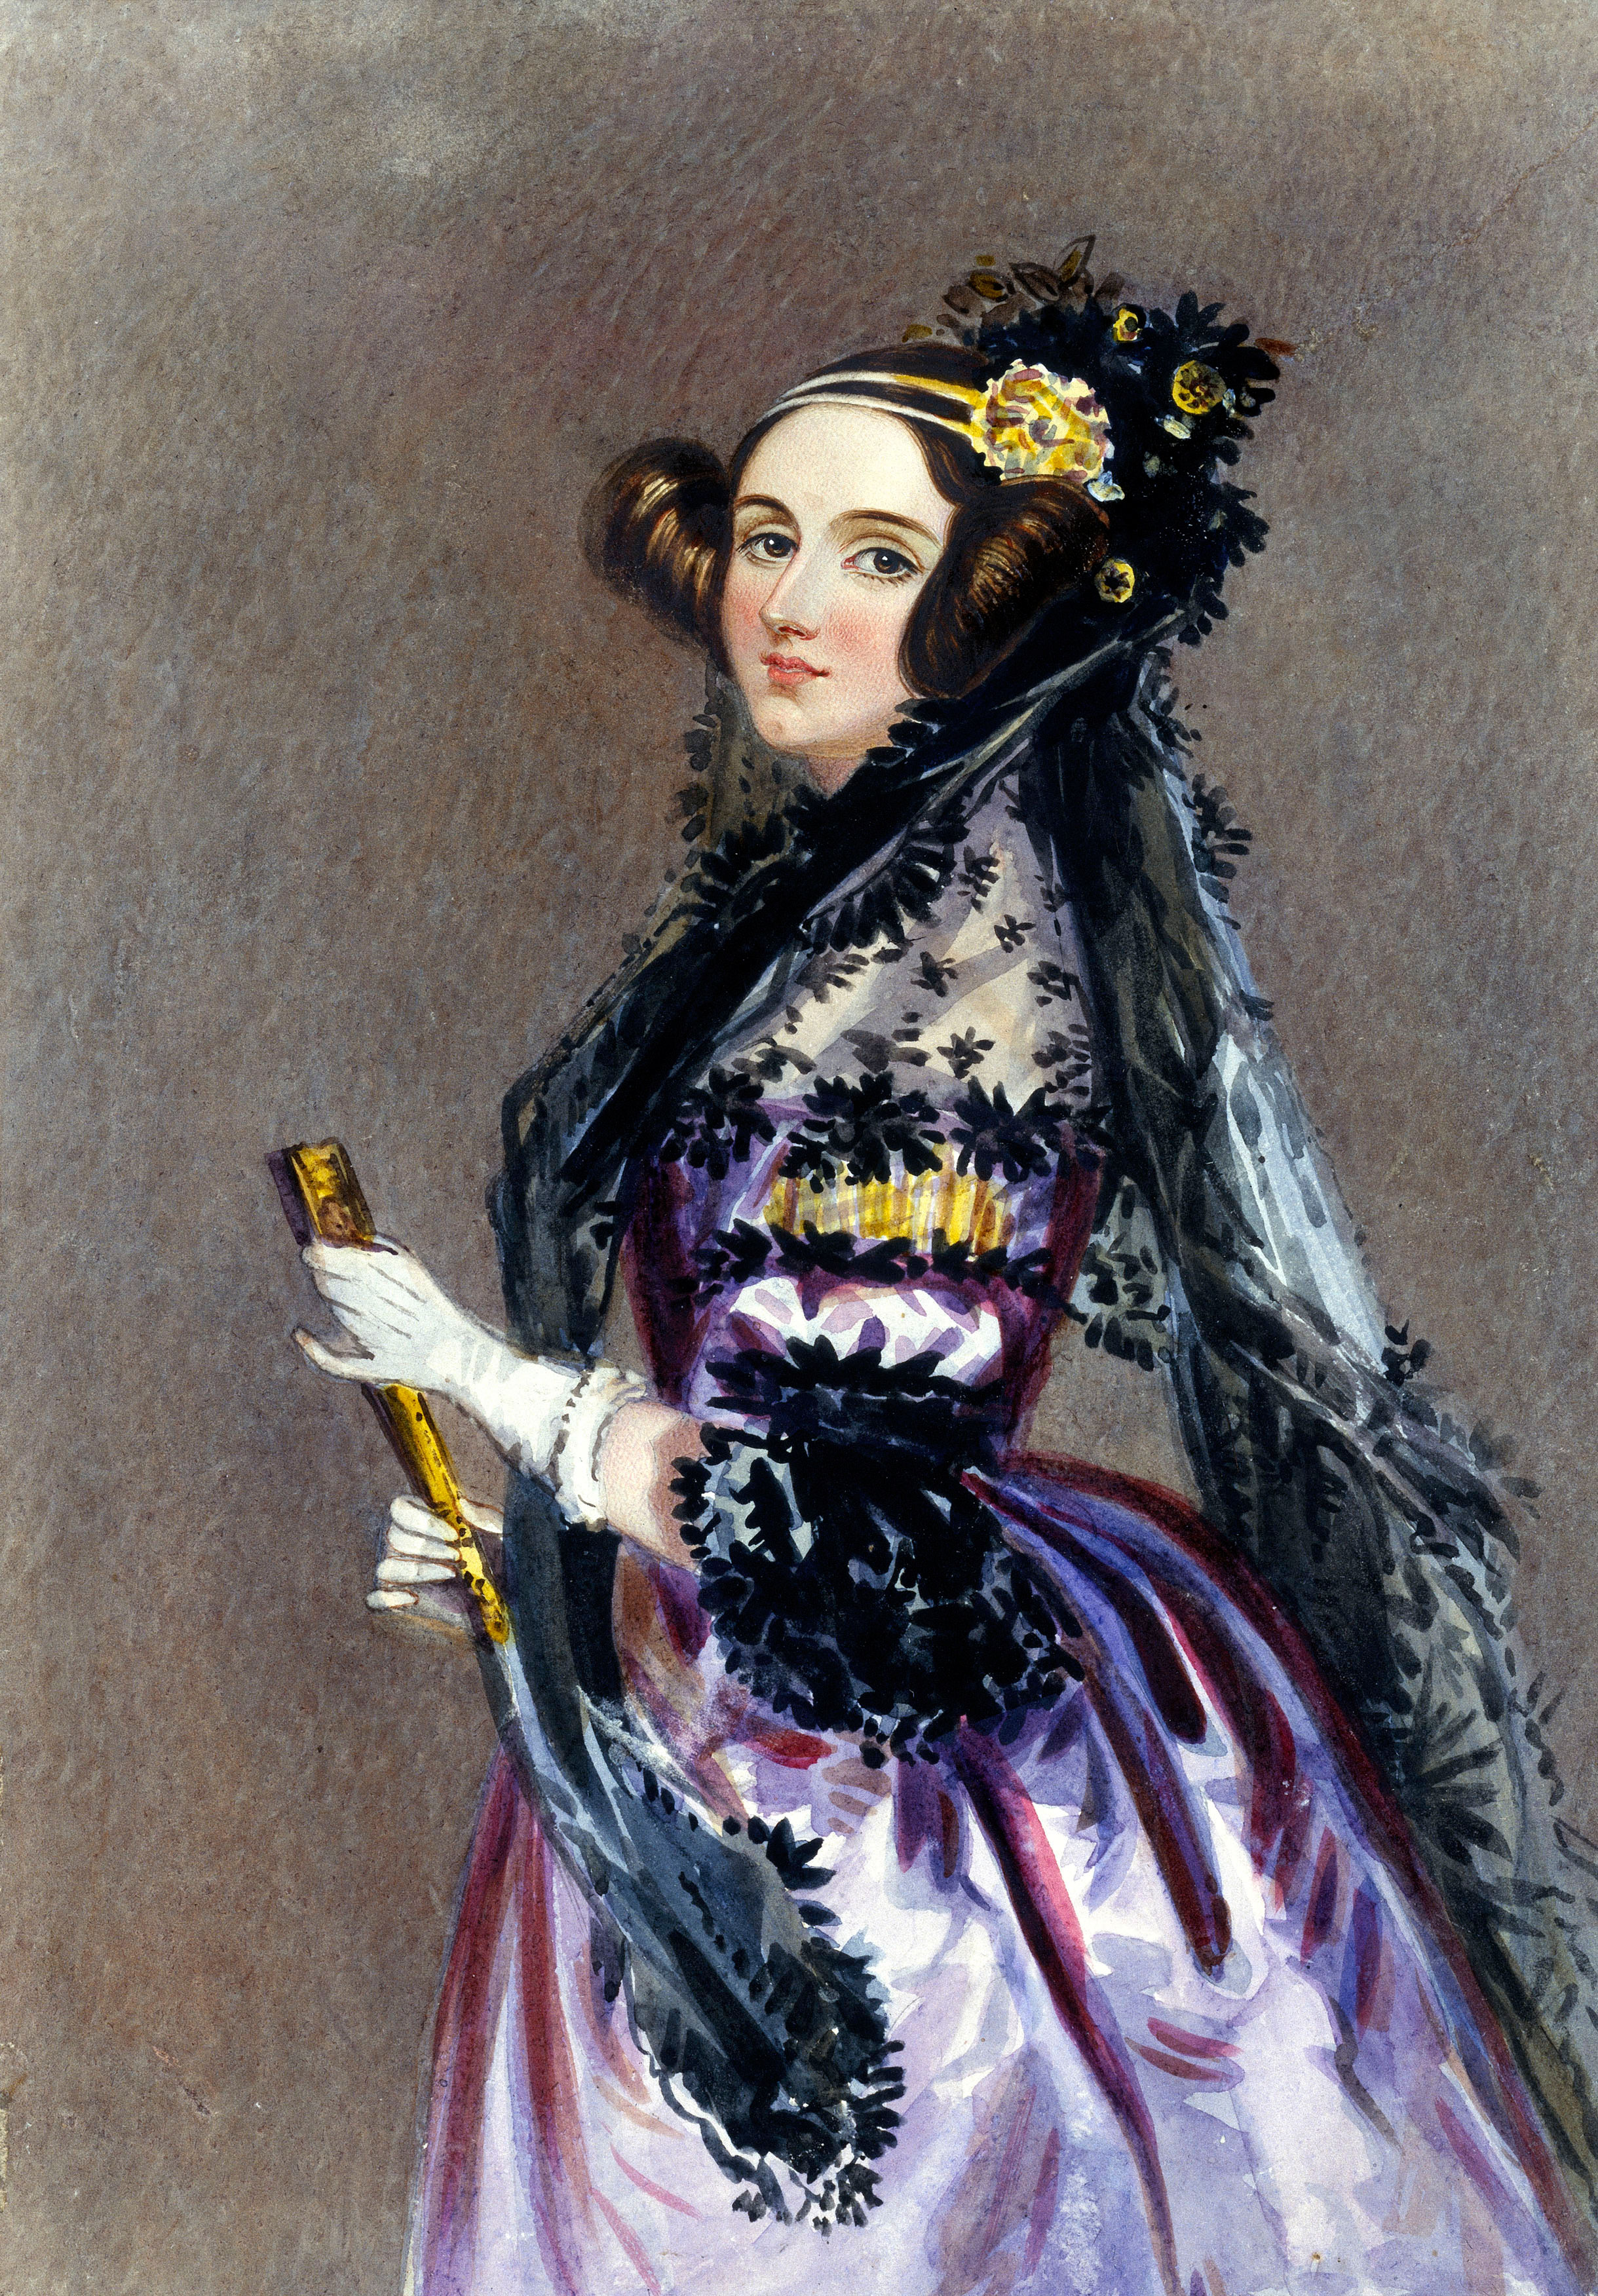
\includegraphics[width=0.4\linewidth]{graphics/Ada_Lovelace_portrait.jpg} % replace the path with your own file
\caption{The portrait of Ada Lovelace.}
\label{fig:ada}
\end{figure}    
\end{lstlisting}
\begin{figure}[ht!]
\centering
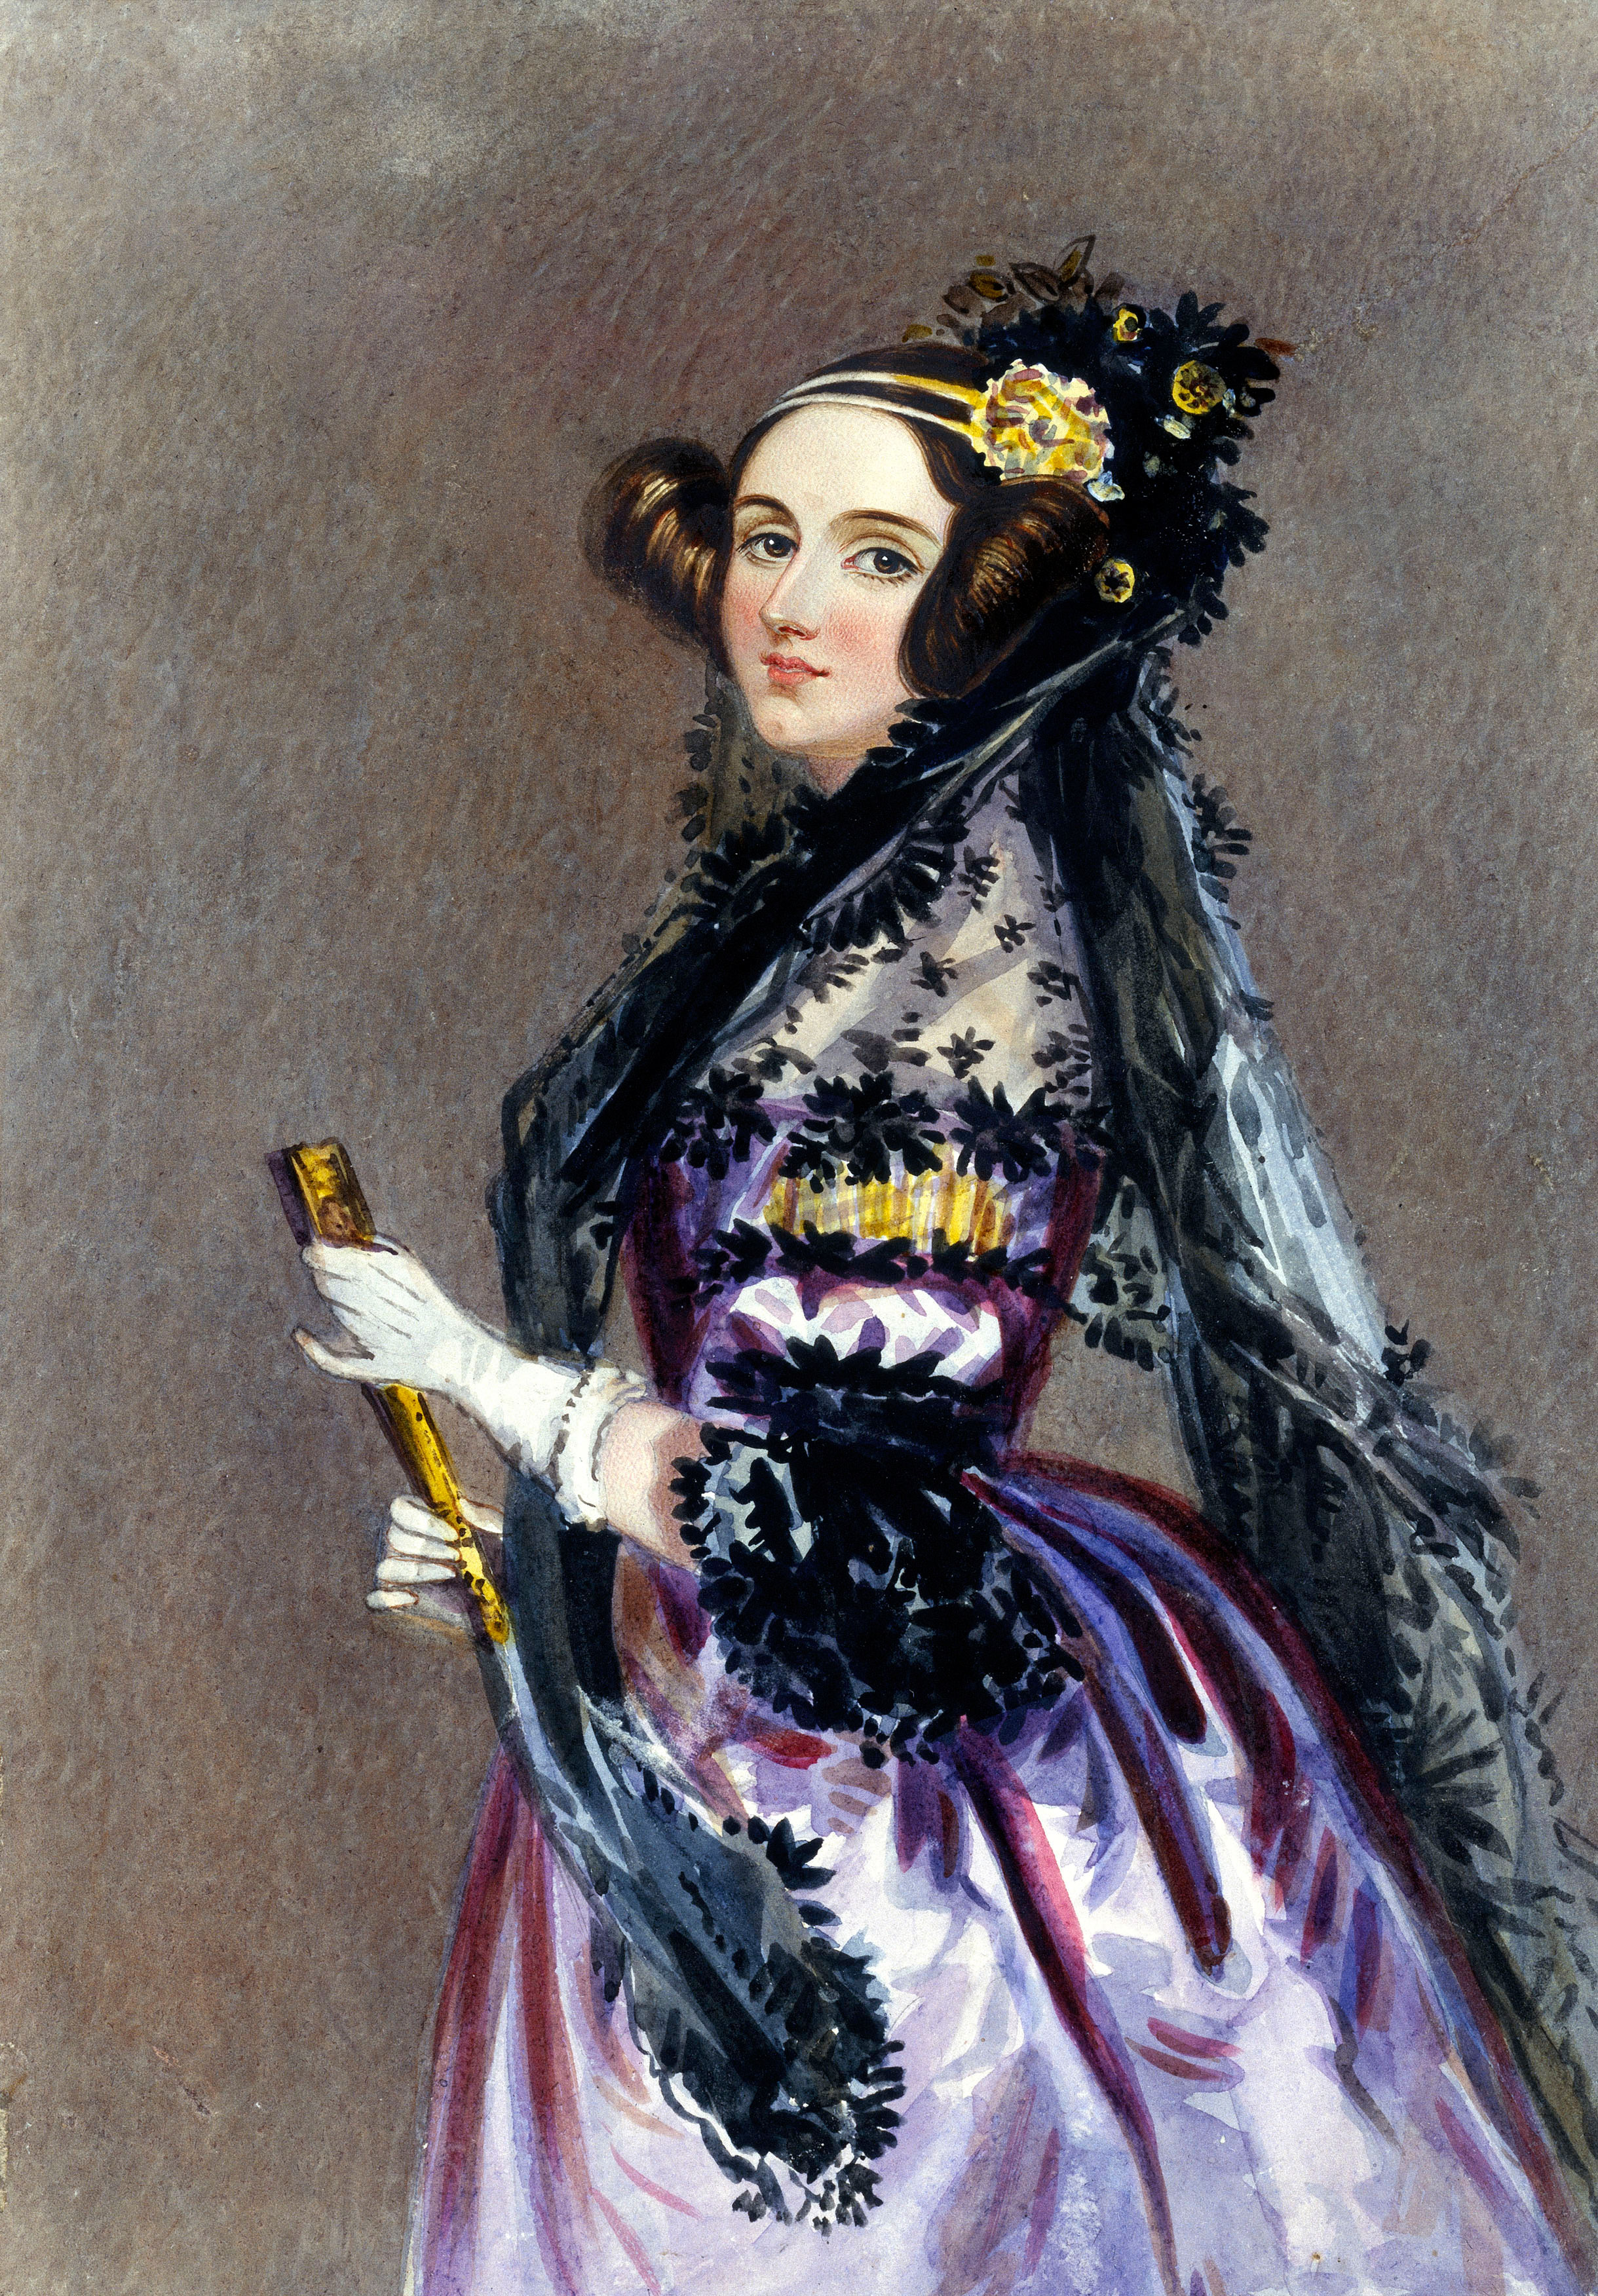
\includegraphics[width=0.4\linewidth]{graphics/Ada_Lovelace_portrait.jpg}
\caption{The portrait of Ada Lovelace.}
\label{fig:ada}
\end{figure}
First, we need to enclose the \texttt{\textbackslash includegraphics} command within a \verb|figure| environment. The \verb|ht!| option indicates that priority is given to put the figure structure exactly in the place where the code is inserted (\verb|h|: here), or at the top of a page (\verb|t|). The \verb|width| option enforces the width of the image to the input value (and similarly there are \verb|height| and \verb|scale|). The \verb|caption| command unsurprisingly generates the caption, while the \verb|label| command works as it is in math mode and allows us to reference it by writing \texttt{\textbackslash ref\{fig:ada\}}.

\paragraph{subcaption}
We can construct a set of subfigures within an overarching figure by utilizing the \verb|subcaption| package and \verb|subfigure| groups. To illustrate, the following code is deployed to generate Figure \ref{fig:TC1}: 
\begin{lstlisting}
\begin{figure}[ht!]
\centering
\begin{subfigure}[b]{0.45\textwidth}
\centering
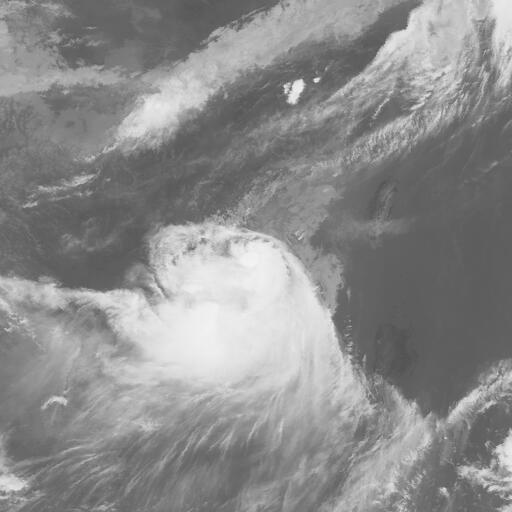
\includegraphics[width=0.8\linewidth]{graphics/MTS108082203.200812.jpg}
\caption{Typhoon Nuri (2008).}
\end{subfigure}
\begin{subfigure}[b]{0.45\textwidth}
\centering
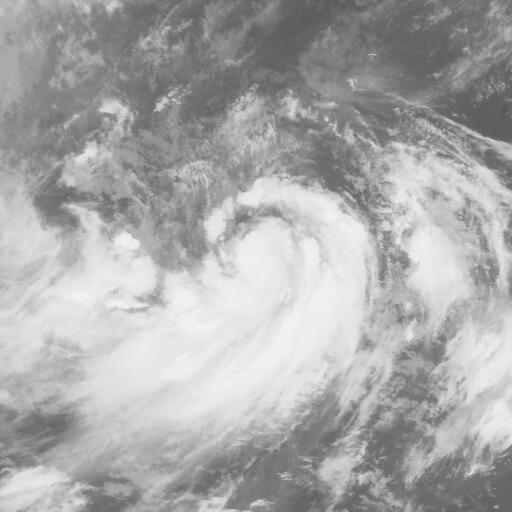
\includegraphics[width=0.8\linewidth]{graphics/MTS212072303.201208.jpg}
\caption{Typhoon Vicente (2012).}
\end{subfigure}
\caption{The infrared satellite images of various Tropical Cyclones affecting Hong Kong.}
\label{fig:TC1}
\end{figure}   
\end{lstlisting}
The \verb|b| option sets the vertical alignment of \verb|subfigure| at the bottom.

\begin{figure}[ht!]
\centering
\begin{subfigure}[b]{0.45\textwidth}
\centering
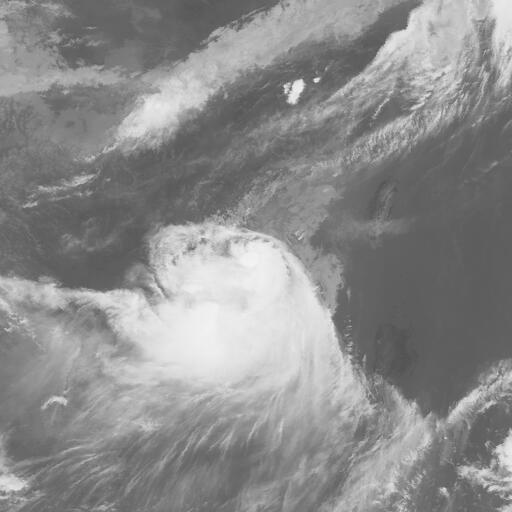
\includegraphics[width=0.8\linewidth]{graphics/MTS108082203.200812.jpg}
\caption{Typhoon Nuri (2008).}
\end{subfigure}
\begin{subfigure}[b]{0.45\textwidth}
\centering
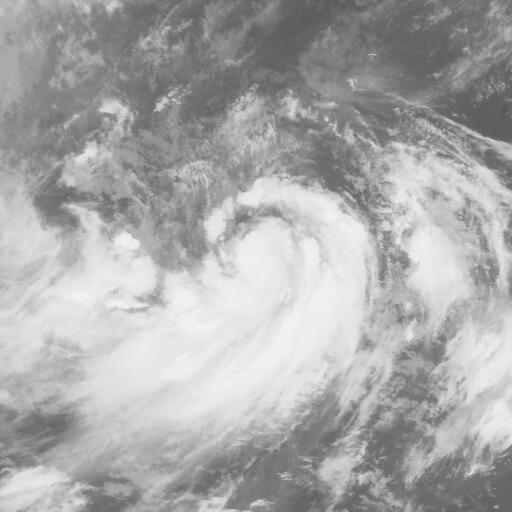
\includegraphics[width=0.8\linewidth]{graphics/MTS212072303.201208.jpg}
\caption{Typhoon Vicente (2012).}
\end{subfigure}
\caption{The infrared satellite images of various Tropical Cyclones affecting Hong Kong. (Source: \href{https://agora.ex.nii.ac.jp/digital-typhoon/index.html.en}{Digital Typhoon})}
\label{fig:TC1}
\end{figure}

\paragraph{ContinuedFloat} To make a longer figure of subfigures that spans multiple pages, we can simply arrange them into separate \verb|figure| environments and call the \texttt{\textbackslash ContinuedFloat} command in all the subsequent \verb|figure| groups. Continuing from the last example, we may have
\begin{lstlisting}
\begin{figure}[hb!]
\ContinuedFloat % here!
\caption{(Cont.) The infrared satellite images of various Tropical Cyclones affecting Hong Kong.}
\centering
\begin{subfigure}[b]{0.45\textwidth}
...
\caption{Typhoon Haima (2016).}
\end{subfigure}
...
\begin{subfigure}[b]{0.45\textwidth}
...
\caption{Typhoon Saola (2023).}
\end{subfigure}
\end{figure}    
\end{lstlisting}
producing
\begin{figure}[hb!]
\ContinuedFloat
\caption{(Cont.) The infrared satellite images of various Tropical Cyclones affecting Hong Kong.}
\centering
\begin{subfigure}[b]{0.45\textwidth}
\centering
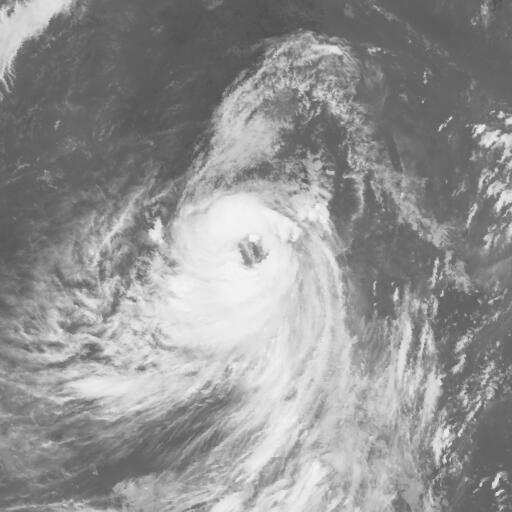
\includegraphics[width=0.8\linewidth]{graphics/HMW816080103.201604.jpg}
\caption{Typhoon Haima (2016).}
\end{subfigure}
\begin{subfigure}[b]{0.45\textwidth}
\centering
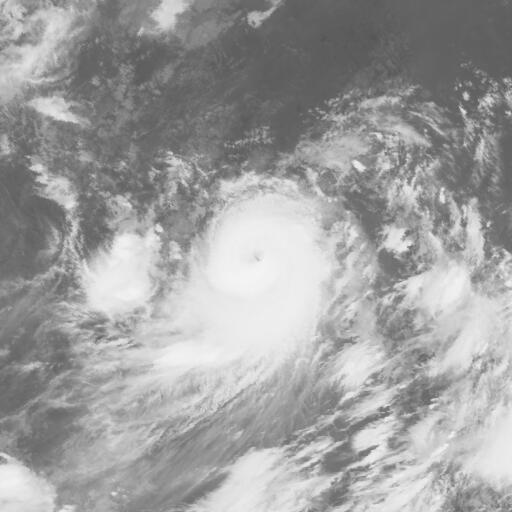
\includegraphics[width=0.8\linewidth]{graphics/HMW817082303.201713.jpg}
\caption{Typhoon Hato (2017).}
\end{subfigure}
\begin{subfigure}[b]{0.45\textwidth}
\centering
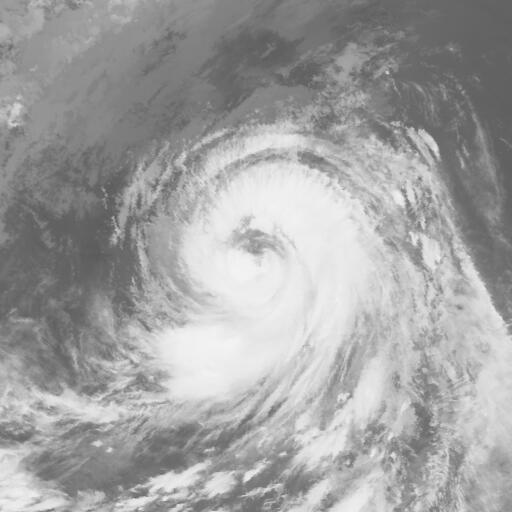
\includegraphics[width=0.8\linewidth]{graphics/HMW818091603.201822.jpg}
\caption{Typhoon Mangkhut (2018).}
\end{subfigure}
\begin{subfigure}[b]{0.45\textwidth}
\centering
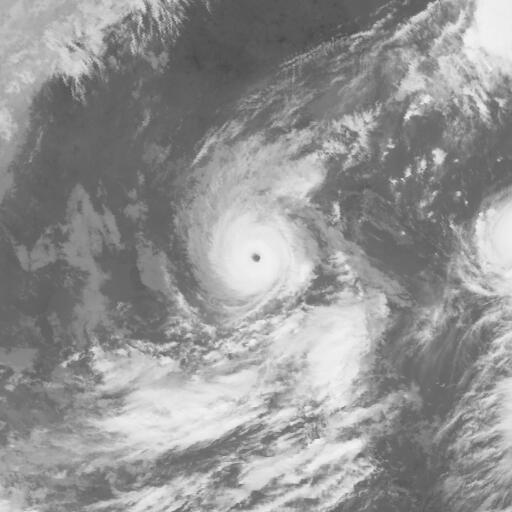
\includegraphics[width=0.8\linewidth]{graphics/HMW923090103.202309.jpg}
\caption{Typhoon Saola (2023).}
\end{subfigure}
\end{figure}

\subsection{Tables}

\paragraph{table, tabularx}
Just like embedding figures, building a table requires us to place the content inside the corresponding \verb|table| environment. While it is possible to use the native \verb|tabular| class for the actual table itself, a more powerful version is provided by the \verb|tabularx| package and its class that bears the same name. This is demonstrated via Table \ref{tab:armyunits} thereafter, which is generated by
\begin{lstlisting}
\begin{table}[ht!]
\centering
\begin{tabularx}{\textwidth}{|l|p{0.55\textwidth}|>{\raggedleft}X|>{\raggedleft\arraybackslash}X|}
\hline
Unit & Description & Attack & Defense \\
\hline
Infantry & The most basic unit and backbone of any army, all-around abilities with a cheap cost. & 20 & 25 \\
\hline
Cavalry & The shock unit in an army with very strong power. & 40 & 30 \\
\hline
Artillery & The support unit that provides bombardment support from far away. & 30 & 5 \\
\hline
\end{tabularx}
\caption{The unit statistics table for a hypothetical game.}
\label{tab:armyunits}
\end{table}
\end{lstlisting}
\begin{table}[ht!]
\centering
\begin{tabularx}{\textwidth}{|l|p{0.55\textwidth}|>{\raggedleft}X|>{\raggedleft\arraybackslash}X|}
\hline
Unit & Description & Attack & Defense \\
\hline
Infantry & The most basic unit and backbone of any army, all-around abilities with a cheap cost. & 20 & 25 \\
\hline
Cavalry & The shock unit in an army with very strong power. & 40 & 30 \\
\hline
Artillery & The support unit that provides bombardment support from far away. & 30 & 5 \\
\hline
\end{tabularx}
\caption{The unit statistics table for a hypothetical game.}
\label{tab:armyunits}
\end{table}
The \verb|ht!| option, \verb|caption|, and \verb|label| work exactly as the figure counterpart. For the \verb|tabularx| group, the first argument indicates the width of the entire table, set to \texttt{\textbackslash textwidth} here. The second argument \texttt{\{|l|p\{0.55\textbackslash textwidth\}|\allowbreak >\{\textbackslash raggedleft\}X|>\{\textbackslash raggedleft\textbackslash arraybackslash\}X|\}} indicates the justification of the columns: the first column is left-aligned (\verb|l|, similarly we have \verb|c| and \verb|r|) and its size will fit the text; the second column (\verb|p|) forces a width of $0.55$ times \texttt{\textbackslash textwidth}; the remaining width is distributed evenly to last two columns (\verb|X|). The part of \texttt{>\{\textbackslash raggedleft\}} is applied to the \verb|X| columns, making them right-aligned.\footnote{\texttt{\textbackslash arraybackslash} is needed in the last column, see \href{https://tex.stackexchange.com/questions/372464/last-tabularx-column-raggedright-with-memoir}{\TeX{} StackExchange 372464}.} Finally, \texttt{|} and \texttt{\textbackslash hline} produce vertical/horiztonal separating lines; \texttt{\&} slices between the columns and \texttt{\textbackslash\textbackslash} marks the end of a row.

Also, note that \texttt{\textbackslash ContinuedFloat} can also be applied to \texttt{table}.

\paragraph{captionbeside} It is also possible to arrange the table so that the caption appears to the side of it. This is done by stacking the \verb|captionbeside| environment provided by KOMA-script. For example, the code
\begin{lstlisting}
\begin{table}[ht]
\begin{captionbeside}{This caption appears to the left of the Fibonacci numbers table.}[l][\textwidth]{
\adjustbox{valign=t}{
    \begin{tabularx}{0.4\textwidth}{|X|X|}
    \hline
    $n$ & $F_n$ \\
    \hline 
    $1$ & $1$ \\
    \hline 
    $2$ & $1$ \\
    \hline 
    $3$ & $2$ \\
    \hline 
    $4$ & $3$ \\
    \hline
    $5$ & $5$ \\
    \hline
    $6$ & $8$ \\
    \hline
    \end{tabularx}}
}
\end{captionbeside}
\label{tab:fib}
\end{table}    
\end{lstlisting}
produces Table \ref{tab:fib} below.

\begin{table}[ht]
\begin{captionbeside}{This caption appears to the left of the Fibonacci numbers table.}[l][\textwidth]{\adjustbox{valign=t}{\begin{tabularx}{0.4\textwidth}{|X|X|}
\hline
$n$ & $F_n$ \\
\hline 
$1$ & $1$ \\
\hline 
$2$ & $1$ \\
\hline 
$3$ & $2$ \\
\hline 
$4$ & $3$ \\
\hline
$5$ & $5$ \\
\hline
$6$ & $8$ \\
\hline
\end{tabularx}}}
\end{captionbeside}
\label{tab:fib}
\end{table}
We fill the caption in the first argument, followed by the relative position of the caption (\verb|l|: left) and the full width of the structure, finally with the actual \verb|tabularx| object. We also have to additionally load the \verb|adjustbox| package and use the corresponding command to tell the table to align itself at the top (\verb|valign=t|). This also requires us to first set the \texttt{\textbackslash KOMAoptions} to take \verb|captions=besidetop| (likewise we have \verb|captions=besidebottom| and more).

\paragraph{Shared Numbering between Figures and Tables}
Sometimes we may want to share the numbering between \textit{floats} (including figures, tables, and so on). This is done by the following patch that can be inserted into the preamble:
\begin{lstlisting}
\makeatletter
\let\c@table\c@figure
\let\ftype@table\ftype@figure
\makeatother
\end{lstlisting}
This involves the primitive \TeX{} functions, so we will not discuss them there. For more information, read \href{https://stackoverflow.com/questions/3865036/using-a-single-count-for-figures-and-tables-in-latex}{StackOverflow 3865036}, and \href{https://tex.stackexchange.com/questions/8351/what-do-makeatletter-and-makeatother-do}{\TeX{} StackExchange 8351} for what the \texttt{\textbackslash makeatletter} and \texttt{\textbackslash makeatother} commands do.

\begin{exercisebox}
\begin{Exercise}
Try to import and load your favorite image into the document. 
\end{Exercise}
\begin{Exercise}
Recreate any one of the tables in Chapter \ref{chap:maths}.
\end{Exercise}
\end{exercisebox}

\section{Minipages and Multiple Columns}

\paragraph{minipage}
Sometimes we may want to partition the content into smaller blocks that are embedded within the current page, and can be placed or ordered (e.g.\ parallel) in the way we want. The \verb|minipage| environment basically acts like a more versatile version of a \verb|parbox| environment and serves this purpose. For example, something like
\begin{lstlisting}
yields \par
\begin{center}
\begin{minipage}[b]{0.48\textwidth}
\lipsum[6]
\end{minipage}
\hfill
\begin{minipage}[b]{0.48\textwidth}
\lipsum[7]
\end{minipage}    
\end{center}      
\end{lstlisting}
yields \par
\begin{center}
\begin{minipage}[b]{0.48\textwidth}
\lipsum[6]
\end{minipage}
\hfill
\begin{minipage}[b]{0.48\textwidth}
\lipsum[7]
\end{minipage}    
\end{center}
The \verb|[b]| option indicates the baseline is set at the bottom, and hence the two blocks will be bottom-aligned, provided that their width is fixed to $0.48$ times \texttt{\textbackslash textwidth} and thus they fit in the main text area.

\paragraph{parcolumns} The \verb|parcolumns| package can also achieve the above effect and is more specialized for typesetting different pieces in two or more parallel columns. It also supports page breaks. Using the same example, we can write
\begin{lstlisting}
\begin{parcolumns}{2}
\colchunk[1]{\lipsum[6]}
\colchunk[2]{\lipsum[7]}
\colplacechunks
\colchunk[1]{\lipsum[8]}
\colchunk[2]{\lipsum[9]}
\end{parcolumns}
\end{lstlisting}
to get\\
\begin{parcolumns}{2}
\colchunk[1]{\lipsum[6]}
\colchunk[2]{\lipsum[7]}
\colplacechunks
\colchunk[1]{\lipsum[8]}
\colchunk[2]{\lipsum[9]}
\end{parcolumns}
where the first argument of the environment clearly indicates the number of columns and the \texttt{\textbackslash colplacechunks} command releases the loaded \texttt{\textbackslash colchunk[<col\allowbreak\_no.>]} and goes to the next paragraph.

\paragraph{multicol} A task closely related to what \verb|parcolumns| does above is to typeset a single, continuous stream of text along multiple columns, like in many academic papers. The \texttt{multicol} package is designed for this and will carry out the automatic splitting. For example, by encapsulating the text inside the \verb|multicols| environment as
\begin{lstlisting}
\begin{multicols}{2}
Zhuge Liang (born 181, Yangdu [now Yinan, Shandong province], China--died August 234, Wuzhangyuan [now in Shaanxi province], China) was a celebrated adviser to Liu Bei, founder of the Shu-Han dynasty (221--263/264).
...
A mechanical and mathematical genius, Zhuge is credited with inventing a bow for shooting several arrows at once and with perfecting the Eight Dispositions, a series of military tactics. In the Sanguozhi yanyi (Romance of the Three Kingdoms), the great 14th-century historical novel, Zhuge is one of the main characters; he is portrayed as being able to control the wind and foretell the future.
\end{multicols}
\end{lstlisting}
(again with the number of columns indicated in the first argument) we may acquire the following layout:
\begin{multicols}{2}
Zhuge Liang (born 181, Yangdu [now Yinan, Shandong province], China--died August 234, Wuzhangyuan [now in Shaanxi province], China) was a celebrated adviser to Liu Bei, founder of the Shu-Han dynasty (221--263/264).

Quick Facts: \\
Wade-Giles romanization: Chu-ko Liang \\
Courtesy name: Kongming \\
Born: 181, Yangdu [now Yinan, Shandong province], China \\
Died: August 234, Wuzhangyuan [now in Shaanxi province], China (aged 53)

Zhuge, to whom supernatural powers often are ascribed, has been a favoured character of many Chinese plays and stories. Legend states that Liu Bei, then a minor military figure, heard of Zhuge Liang’s great wisdom and came three times to the wilderness retreat to which Zhuge had retired to seek him out as an adviser. It is known that Zhuge helped Liu organize a large army and found a dynasty. Liu was so impressed with Zhuge’s wisdom that on his deathbed Liu urged his son to depend on Zhuge’s advice and urged Zhuge to ascend the throne himself if the prince were unable to rule. Some historical accounts indicate that Zhuge died from illness while leading a military campaign in 234.

A mechanical and mathematical genius, Zhuge is credited with inventing a bow for shooting several arrows at once and with perfecting the Eight Dispositions, a series of military tactics. In the Sanguozhi yanyi (Romance of the Three Kingdoms), the great 14th-century historical novel, Zhuge is one of the main characters; he is portrayed as being able to control the wind and foretell the future. (Source: Encyclopaedia Britannica)
\end{multicols}


\paragraph{twocolumn} We can also pass the \verb|twocolumn=true| option to \texttt{\textbackslash KOMAoptions} to demand the entire book to be formatted in two columns globally. However, note that it will greatly mess up the layout of this book. (The decision to adopt such a format should be made at an early time!)
\chapter{Self-defined Commands and Environments}

\section{Self-defined Commands}

\section{If-then-else Statements}

\section{Self-defined Environments}
\chapter{More on Book Layout Design}

\paragraph{Introduction}
This chapter will go into the details about designing and refining the layout of a \LaTeX{} book, including how to edit the page style with running headers/footers, chapter/section headings, a good-looking title page, and more.

\section{Page Configuration}

\subsection{Some Universal Settings for the Pages}

\paragraph{twoside}
In a printed book, there will be a distinction between odd (right) and even (left) pages, i.e.\ \textit{two-sided}, whereas an electronic PDF document is usually \textit{one-sided} and has no such issue. To choose one of these configurations in a \texttt{scrbook}, we can change the \texttt{twoside} parameter in \texttt{\textbackslash KOMAoptions} to \texttt{false}, \texttt{semi}, or \texttt{true}. Unsurprisingly, \texttt{false} indicates one-sided and \texttt{true} means two-sided. Being two-sided means that there will be a difference between the inner/outer margins, with the outer margin (left/right on even/odd pages) occupying two times the space as the inner one. The running headers on odd and even pages will also show the current section/chapter differently.

In this book, the \texttt{twoside} option is set to \texttt{semi} by adding \texttt{\textbackslash KOMAoptions\allowbreak\{twoside=semi\}}. This retains equal margins as if the document is one-sided, but the headers will switch alternately just like two-sided.

\paragraph{DIV}
The extent of the type area in pages is controlled by the \texttt{DIV} factor passed to \texttt{\textbackslash KOMAoptions}. The higher the value of \texttt{DIV}, the larger the fraction of the main text area and the smaller the margins. The reference value of \texttt{DIV} usually ranges from $9$ to $12$. However, we can delegate the calculation of an optimal \texttt{DIV} by setting \texttt{DIV} to either \texttt{calc} or \texttt{classic}. If a new font is loaded, it is also desirable to recalculate an appropriate type area by calling \texttt{\textbackslash KOMAoptions\{DIV=last\}} that reuses the same setting.

\paragraph{linespread}
Finally, to control the \textit{line spread} in the main text, just add \texttt{\textbackslash linespread\{<value>\}}. Here it is set to $1.25$.

\subsection{Page Style}

\paragraph{Headers and Footers}
A very important part of a page is its \textit{header} and \textit{footer}. Editing the content within a header/footer requires us to load the \texttt{scrlayer-\allowbreak scrpage} package. The default page style for the main content in the book is invoked by \texttt{\textbackslash pagestyle\{scrheadings\}}. We can refer the inner/center/outer header/footer via \texttt{ihead}, \texttt{chead}, \texttt{ohead}, \texttt{ifoot}, \texttt{cfoot}, and \texttt{ofoot} correspondingly. For example, the default page number is put at the outer footer, and this book has moved it to the center footer by declaring:
\begin{lstlisting}
\pagestyle{scrheadings}
\ofoot*{}
\cfoot*{\pagemark}    
\end{lstlisting}
where the variable \texttt{\textbackslash pagemark} stores the page number in \texttt{scrbook}.

There is also a finer division between even/odd pages for headers/footers: \texttt{lehead}, \texttt{cehead}, \texttt{rehead}, \texttt{lohead}, \texttt{cohead}, \texttt{rohead}, where \texttt{l}, \texttt{c}, \texttt{r} stand for left/center/right, and \texttt{e}, \texttt{o} represent even and odd respectively. If we want to swap the chapter and section in the even/odd-paged headers, we can write something like
\begin{lstlisting}
\lehead*[]{\rightmark}
\rohead*[]{\leftmark}    
\end{lstlisting}
The optional argument will be applied to the chapter page (more accurately, the \textit{plain} page style), and is left empty as in the default setting. The \texttt{\textbackslash leftmark} and \texttt{\textbackslash rightmark} hold the original left/right headers, the depth of which is controlled by
\begin{lstlisting}
\automark[section]{chapter} % [right]{left}
\end{lstlisting}

\paragraph{setkomafont}
Now we will further customize the font style and color of our header by the command \texttt{\textbackslash setkomafont\{<element>\}\{<commands>\}}. As its name suggests, it applies commands to set up a certain element in a page. For headers, the corresponding alias is \texttt{pagehead}, and in this book, we have
\begin{lstlisting}
\setkomafont{pagehead}{\color{RoyalBlue}\slshape\bfseries}    
\end{lstlisting}
Many other elements can be changed as well, including \texttt{chapter}, \texttt{section}, \texttt{footnote}, \texttt{caption}, \texttt{pagefoot}, and so on.

\paragraph{headsepline}
The separating line under the header is added via passing the switch \texttt{headsepline=on} to \texttt{\textbackslash KOMAoptions}. We similarly have \texttt{footsepline}.

\paragraph{chaptermarkformat}
Sometimes we may want to change the chapter label in the header too. This is done by applying \texttt{\textbackslash renewcommand*} to \texttt{\textbackslash chaptermarkformat}. In this book, we have
\begin{lstlisting}
\renewcommand*{\chaptermarkformat}{\chapapp~\thechapter\autodot~--~} % ~ occupies a space, -- is a dash
\end{lstlisting}
\texttt{\textbackslash chapapp} stores the word "Chapter", \texttt{\textbackslash thechapter} contains the current chapter counter, and \texttt{\textbackslash autodot} is empty, reserved for an extra dot after any chapter/section numbering. As you may have guessed, there is also \texttt{\textbackslash sectionmarkformat}.

\begin{exercisebox}
\begin{Exercise}
Edit the page style to make your own header and footer.
\end{Exercise}
\end{exercisebox}

\section{Appearance of Chapters and Sections}

\paragraph{chapterprefix, chapterformat}
We can single out the chapter number as a prefix in the chapter title by setting \texttt{chapterprefix=true} in \texttt{\textbackslash KOMAoptions}. Furthermore, we can customize it by \texttt{\textbackslash addtokomafont} which behaves similarly as \texttt{\textbackslash setkomafont}:
\begin{lstlisting}
\addtokomafont{chapterprefix}{\itshape\color{white}}
\end{lstlisting}
In addition, we can again call \texttt{\textbackslash renewcommand*} to manipulate \texttt{\textbackslash chapterformat}. In this book, the following code is adopted:
\begin{lstlisting}
\renewcommand*{\chapterformat}{\raggedleft\colorbox{RoyalBlue}{\parbox[b][2.8em]{2.8em}{\vfill\centering{\large\chapapp}\\[-0.4em]\thechapter\vfill}}}  
\end{lstlisting}

\paragraph{sectionformat}
In the same way, we have \texttt{\textbackslash sectionformat} that can be edited for section headings. The code to produce the white section number in a black box is
\begin{lstlisting}
\renewcommand*{\sectionformat}{\colorbox{black}{\textcolor{white}{\thesection}}\enskip}    
\end{lstlisting}
where \texttt{\textbackslash enskip} denotes a space as wide as half an em.

\paragraph{sectionlinesformat}
Meanwhile, the black line under the section headings is governed by \texttt{\textbackslash sectionlinesformat}. It has to accept $4$ arguments, where only the third (section number) and the last (section name) will be relevant here:
\begin{lstlisting}
\renewcommand*{\sectionlinesformat}[4]{\makebox[0pt][l]{\rule[-\fboxsep]{\textwidth}{1pt}}#3\parbox[b]{0.85\textwidth}{\linespread{1}\selectfont#4}}
\end{lstlisting}
The \texttt{makebox} command creates an artificial empty box that does not occupy any width ($0$ pt) and contains the desired separating line (\texttt{\textbackslash rule} with a length of \texttt{\textbackslash textwidth}). It is vertically offset downwards by \texttt{\textbackslash fboxsep} to compensate for the padding around the black numbering box (\texttt{\#3}) that follows, defined via \texttt{\textbackslash sectionformat} above. The section name (\texttt{\#4}) is subsequently wrapped by a \texttt{\textbackslash parbox} that is bottom-aligned and can account for any title longer than one line.

\paragraph{chapterheadendvskip}
While there is also the \texttt{\textbackslash chapterlinesformat} command for making a line below the chapter title, we can achieve more by tackling \texttt{\textbackslash chapterheadendvskip} instead. It controls the stuff (usually some vertical skip) that occurs after a chapter heading. For aesthetics, we will load the \texttt{pgfornament} package that supplies many beautiful visual patterns. Then, we can write
\begin{lstlisting}
\renewcommand*{\chapterheadendvskip}{\pgfornament[width=\textwidth]{88}\par} % the 88th ornament
\end{lstlisting}
to achieve the layout present in the book.

\paragraph{chapterheadstartvskip}
There exists the \texttt{\textbackslash chapterheadstartvskip} counterpart for anything before the chapter title as well. The default vertical space above the chapter heading may be too much, and we can shorten it via 
\begin{lstlisting}
\renewcommand*{\chapterheadstartvskip}{\addvspace{2em}}    
\end{lstlisting}
\texttt{\textbackslash addvspace} is a variant of \texttt{\textbackslash vspace}, which is a kind of rubber length: it adds just enough vertical space so that the total space is as large as the input length if the existing space is shorter than that, and does nothing when it is already long enough.

\paragraph{sfdefaults} As you may notice, the chapter/section headings are written in sans-serif. To change this, we can set \texttt{sfdefaults} to \texttt{no} in \texttt{\textbackslash KOMAoptions}. We can also mark up text with \texttt{\textbackslash textmaybesf\{<text>\}} that is toggled by  \texttt{sfdefaults} too.

\section{Title Page and Front/Back Matter}

\paragraph{Title Page}
The easiest way to generate a \textit{title page} is to simply use the \texttt{\textbackslash maketitle} command. Just enter the book (sub)title, author name, and the like in the preamble using the corresponding commands, for example:
\begin{lstlisting}
\title{How to Reproduce this Book Exactly with \LaTeX}
\subtitle{A Self-contained Tutorial on Writing Mathematical Notes}
\author{C.~L.~Loi}
\end{lstlisting}
and maybe \texttt{\textbackslash date} and \texttt{\textbackslash publishers}, etc. Then calling \texttt{\textbackslash maketitle} will automatically build a title page for you. In addition, the \texttt{titlepage} switch in \texttt{\textbackslash KOMAoptions} can decide if it is embedded in-page. However, it is more flexible to design our own title page using the \texttt{titlepage} environment. In this book, we have adopted:
\begin{lstlisting}
\begin{titlepage}
\parbox{0.7\textwidth}{\Huge\raggedright\textbf{\textmaybesf{How to Reproduce this Book Exactly with \LaTeX}}}\par
\vspace{2mm}
\parbox[b]{0.9\textwidth}{\large\raggedright\textit{A Self-contained Tutorial on Writing Mathematical Notes}}
\hfill\textcolor{RoyalBlue}{\rule{3mm}{3mm}}\par
\vspace{4mm}\hrule\par
{\Large\raggedleft\textmaybesf{v1.0.0}\hfill C.~L.~Loi\par}
\vfill
{\large\raggedleft A student from \\ 
CUHK-EESC/NTU-AS\par}
\end{titlepage}
\end{lstlisting}

\paragraph{Front/Main/Back Matter} Usually in a book, there will be \textit{front matter} (title page, preface, table of contents) and \textit{back matter} (bibliography, index). To mark them, just write \texttt{\textbackslash frontmatter} and \texttt{\textbackslash backmatter} in front of the corresponding parts. We also have \texttt{\textbackslash mainmatter} for transitioning to the main content. So it should look like
\begin{lstlisting}
\frontmatter
\begin{titlepage}
\parbox{0.7\textwidth}{\Huge\raggedright\textbf{\textmaybesf{How to Reproduce this Book Exactly with \LaTeX}}}\par
\vspace{2mm}
\parbox[b]{0.9\textwidth}{\large\raggedright\textit{A Self-contained Tutorial on Writing Mathematical Notes}}
\hfill\textcolor{RoyalBlue}{\rule{3mm}{3mm}}\par
\vspace{4mm}\hrule\par
{\Large\raggedleft\textmaybesf{v1.0.0}\hfill C.~L.~Loi\par}
\vfill
{\large\raggedleft A student from \\ 
CUHK-EESC/NTU-AS\par}
\end{titlepage}
\thispagestyle{empty}
\vspace*{\fill}
"How to Reproduce this Book Exactly with \LaTeX"\\
Copyright ©, C.~L.~Loi, 2025. All rights reserved.
\tableofcontents

\mainmatter
\chapter{The Basic Set-up and Structure of a \LaTeX{} Book}

\paragraph{Introduction}
The first chapter discusses how to properly configure \LaTeX{} files and organize the content's structure so that we can generate our first readable \LaTeX{} book PDF. 

\section{Class, Commands, Options, and Packages}
\label{sec:komaopt}

\paragraph{Class}
For each \LaTeX{} document, we need to specify its \textit{class}. Throughout this book, we will use the \verb|scrbook| class provided by the \textbf{KOMA-Script}. To do so, we write \texttt{\textbackslash documentclass\{scrbook\}} at the very beginning (\textit{preamble}) of the main \TeX{} file. Although not explored in this book, some other notable classes that may be of use include \verb|beamer|, \verb|moderncv|, and \verb|article| (or \verb|scrartcl|).

\paragraph{Commands and Options} The \verb|scrbook| class provides several \textit{options} to customize the format of the book. We can either supply the arguments when declaring the class, or use the command \texttt{\textbackslash KOMAoptions} in the preamble. A \textit{command} works like a function in common programming languages and performs some specific action. Commands in \LaTeX{} are denoted by the backslash \verb|\| as the first character. In this book, we have used
\begin{lstlisting}
\KOMAoptions{paper=a4, fontsize=12pt, chapterprefix=true, twoside=semi, DIV=classic, parskip=half}
\end{lstlisting}
The arguments are typed inside the curly brackets \verb|{}| following the name of the command. Clearly, the \verb|paper| option requires the pages to be in A4 size while \verb|fontsize| indicates that the font is 12 pt large. The remaining options will be explained as we go through the later chapters.

\paragraph{Packages} To enable extra functionalities, we need to import \textit{packages}. We can write along the lines of \texttt{\textbackslash usepackage[<options>]\{<package\_name>\}} in the preamble to do so. We will not list all the required packages now at once, but only when they are needed. The first package we usually need is the \verb|fontenc| package with the \verb|T1| option, flagged inside a pair of square brackets.

\begin{exercisebox}
\begin{Exercise}
Try to import the \verb|fontenc| package with the \verb|T1| option as suggested above. There may not be any noticeable difference, but at least you should not be receiving errors.
\end{Exercise}
\begin{Exercise}
Also, try to use \texttt{\textbackslash documentclass[<options>]\{scrbook\}} instead of the \texttt{\textbackslash KOMAoptions} command to achieve the same class setting.
\end{Exercise}
\end{exercisebox}

\section{Structure Hierarchy}

\subsection{Chapters and (Sub-)Sections}

\paragraph{Chapters, Sections} As in any other book, the entire content is divided into \textit{chapters}, which in turn usually consist of several \textit{sections}. To mark the beginning of a chapter or section, we place the commands \texttt{\textbackslash chapter\{<chapter\_name>\}} or \texttt{\textbackslash section\{<section\_name>\}} within the \verb|document| environment, which contains the main content and is marked by a pair of \verb|begin| and \verb|end| declarations. The preamble has to be inserted before \verb|document|. So, to typeset the very first section at the start, we write
\begin{lstlisting}
<preamble before the main document>
\begin{document}
...
\chapter{The Basic Set-up and Structure of a \LaTeX{} Book}
...
\section{Class, Options, and Packages}
\paragraph{Class}
For each \LaTeX{} document, we need to specify its \textit{class}. Throughout this book, ...
...
\end{document}
\end{lstlisting}
The \LaTeX{} system updates the chapter/section's numbering internally. The \texttt{\textbackslash textit\{<text>\}} command presents the text in italic shape.

\paragraph{Subsections, Paragraphs} An attentive reader may have already figured out that it is possible to stack an extra layer (a \textit{subsection}) in the hierarchy. This is aptly done not long ago by the \texttt{\textbackslash subsection\{<section\_name>\}} command:
\begin{lstlisting}
\section{Structure Hierarchy}

\subsection{Chapters and (Sub-)Sections}

\paragraph{Chapters, Sections} As in any other book, the entire content is divided into \textit{chapters}, ...
\end{lstlisting}
He/she may also notice that we have used the \texttt{\textbackslash paragraph} command a few times to attach an unnumbered heading for each \textit{paragraph}. There are also starred versions like \texttt{\textbackslash chapter*\{<chapter\_name>\}}, \texttt{\textbackslash section*\{<section\_name>\}}, \texttt{\textbackslash subsection*\{<section\_name>\}}, and so on, which neither display nor increase the numbering/counters.

\subsection{Generating Table of Contents}

\paragraph{Table of Contents}
After establishing the structure of the book, it is convenient to generate a \textit{table of contents (TOC)} as well. In the \verb|scrbook| class, it is easily done by adding the command \texttt{\textbackslash tableofcontents} within the main \verb|document| group. To control the depth of layers shown, we can call \texttt{\textbackslash setcounter{tocdepth}\allowbreak\{<integer>\}} in the preamble, where the \verb|integer| usually ranges from $-1$ to $3$ ($0$: chapters, $1$: sections, $2$: subsections).

\begin{exercisebox}
\begin{Exercise}
Try to add some (numbered or unnumbered) chapters, sections, subsections, or even subsubsections (which are, not surprisingly, produced by \texttt{\textbackslash subsubsection}) to see how they are displayed in the book. You may want to check out \texttt{\textbackslash part}.
\end{Exercise}
\begin{Exercise}
As a follow-up to the last exercise, turn on the table of contents and confirm how the new entries are linked to it. Also, try to adjust the value for \texttt{\textbackslash setcounter{tocdepth}} as proposed above to see the effect.
\end{Exercise}
\end{exercisebox}

\subsection{Organizing the \TeX{} Files behind the Scenes}
\label{subsection:TeXorg}
\paragraph{include} As the size of the project scales up, it is often helpful to keep the files arranged in a clean order for maintenance. We can put the content of each chapter into separate \TeX{} files, and then use the \texttt{\textbackslash include\{<tex\_file\_name>\}} command to import them into the main script. For example, this chapter is stored as \texttt{ch1\_basic\_structure.tex} in my project space, and in the main \TeX{} file, we shall write something like
\begin{lstlisting}
<preamble>
\begin{document}

\tableofcontents
\chapter{The Basic Set-up and Structure of a \LaTeX{} Book}

\paragraph{Introduction}
The first chapter discusses how to properly configure \LaTeX{} files and organize the content's structure so that we can generate our first readable \LaTeX{} book PDF. 

\section{Class, Commands, Options, and Packages}
\label{sec:komaopt}

\paragraph{Class}
For each \LaTeX{} document, we need to specify its \textit{class}. Throughout this book, we will use the \verb|scrbook| class provided by the \textbf{KOMA-Script}. To do so, we write \texttt{\textbackslash documentclass\{scrbook\}} at the very beginning (\textit{preamble}) of the main \TeX{} file. Although not explored in this book, some other notable classes that may be of use include \verb|beamer|, \verb|moderncv|, and \verb|article| (or \verb|scrartcl|).

\paragraph{Commands and Options} The \verb|scrbook| class provides several \textit{options} to customize the format of the book. We can either supply the arguments when declaring the class, or use the command \texttt{\textbackslash KOMAoptions} in the preamble. A \textit{command} works like a function in common programming languages and performs some specific action. Commands in \LaTeX{} are denoted by the backslash \verb|\| as the first character. In this book, we have used
\begin{lstlisting}
\KOMAoptions{paper=a4, fontsize=12pt, chapterprefix=true, twoside=semi, DIV=classic, parskip=half}
\end{lstlisting}
The arguments are typed inside the curly brackets \verb|{}| following the name of the command. Clearly, the \verb|paper| option requires the pages to be in A4 size while \verb|fontsize| indicates that the font is 12 pt large. The remaining options will be explained as we go through the later chapters.

\paragraph{Packages} To enable extra functionalities, we need to import \textit{packages}. We can write along the lines of \texttt{\textbackslash usepackage[<options>]\{<package\_name>\}} in the preamble to do so. We will not list all the required packages now at once, but only when they are needed. The first package we usually need is the \verb|fontenc| package with the \verb|T1| option, flagged inside a pair of square brackets.

\begin{exercisebox}
\begin{Exercise}
Try to import the \verb|fontenc| package with the \verb|T1| option as suggested above. There may not be any noticeable difference, but at least you should not be receiving errors.
\end{Exercise}
\begin{Exercise}
Also, try to use \texttt{\textbackslash documentclass[<options>]\{scrbook\}} instead of the \texttt{\textbackslash KOMAoptions} command to achieve the same class setting.
\end{Exercise}
\end{exercisebox}

\section{Structure Hierarchy}

\subsection{Chapters and (Sub-)Sections}

\paragraph{Chapters, Sections} As in any other book, the entire content is divided into \textit{chapters}, which in turn usually consist of several \textit{sections}. To mark the beginning of a chapter or section, we place the commands \texttt{\textbackslash chapter\{<chapter\_name>\}} or \texttt{\textbackslash section\{<section\_name>\}} within the \verb|document| environment, which contains the main content and is marked by a pair of \verb|begin| and \verb|end| declarations. The preamble has to be inserted before \verb|document|. So, to typeset the very first section at the start, we write
\begin{lstlisting}
<preamble before the main document>
\begin{document}
...
\chapter{The Basic Set-up and Structure of a \LaTeX{} Book}
...
\section{Class, Options, and Packages}
\paragraph{Class}
For each \LaTeX{} document, we need to specify its \textit{class}. Throughout this book, ...
...
\end{document}
\end{lstlisting}
The \LaTeX{} system updates the chapter/section's numbering internally. The \texttt{\textbackslash textit\{<text>\}} command presents the text in italic shape.

\paragraph{Subsections, Paragraphs} An attentive reader may have already figured out that it is possible to stack an extra layer (a \textit{subsection}) in the hierarchy. This is aptly done not long ago by the \texttt{\textbackslash subsection\{<section\_name>\}} command:
\begin{lstlisting}
\section{Structure Hierarchy}

\subsection{Chapters and (Sub-)Sections}

\paragraph{Chapters, Sections} As in any other book, the entire content is divided into \textit{chapters}, ...
\end{lstlisting}
He/she may also notice that we have used the \texttt{\textbackslash paragraph} command a few times to attach an unnumbered heading for each \textit{paragraph}. There are also starred versions like \texttt{\textbackslash chapter*\{<chapter\_name>\}}, \texttt{\textbackslash section*\{<section\_name>\}}, \texttt{\textbackslash subsection*\{<section\_name>\}}, and so on, which neither display nor increase the numbering/counters.

\subsection{Generating Table of Contents}

\paragraph{Table of Contents}
After establishing the structure of the book, it is convenient to generate a \textit{table of contents (TOC)} as well. In the \verb|scrbook| class, it is easily done by adding the command \texttt{\textbackslash tableofcontents} within the main \verb|document| group. To control the depth of layers shown, we can call \texttt{\textbackslash setcounter{tocdepth}\allowbreak\{<integer>\}} in the preamble, where the \verb|integer| usually ranges from $-1$ to $3$ ($0$: chapters, $1$: sections, $2$: subsections).

\begin{exercisebox}
\begin{Exercise}
Try to add some (numbered or unnumbered) chapters, sections, subsections, or even subsubsections (which are, not surprisingly, produced by \texttt{\textbackslash subsubsection}) to see how they are displayed in the book. You may want to check out \texttt{\textbackslash part}.
\end{Exercise}
\begin{Exercise}
As a follow-up to the last exercise, turn on the table of contents and confirm how the new entries are linked to it. Also, try to adjust the value for \texttt{\textbackslash setcounter{tocdepth}} as proposed above to see the effect.
\end{Exercise}
\end{exercisebox}

\subsection{Organizing the \TeX{} Files behind the Scenes}
\label{subsection:TeXorg}
\paragraph{include} As the size of the project scales up, it is often helpful to keep the files arranged in a clean order for maintenance. We can put the content of each chapter into separate \TeX{} files, and then use the \texttt{\textbackslash include\{<tex\_file\_name>\}} command to import them into the main script. For example, this chapter is stored as \texttt{ch1\_basic\_structure.tex} in my project space, and in the main \TeX{} file, we shall write something like
\begin{lstlisting}
<preamble>
\begin{document}

\tableofcontents
\include{ch1_basic_structure}
...
\end{document}
\end{lstlisting}

\section{Testing the Book Layout by Lipsum}

\paragraph{Dummy Text} Sometimes we may need to insert some placeholder text into the code to test how well the book will look in a specific layout. In this case, we can borrow the standard dummy text \textit{Lorem Ipsum} (or in short \textit{Lipsum}) widely used by the community. Just import the \verb|lipsum| generator package, and add \texttt{\textbackslash lipsum[<paragraph\_no.>]} to the desired positions. For example, the code segment
\begin{lstlisting}
...
produces the following text exactly: \par
\lipsum[1-2]
\end{lstlisting}
produces the following text exactly: \par
\lipsum[1-2] \par
The \texttt{\textbackslash par} command signals the end of a paragraph and appends a vertical line spacing afterwards. 
...
\end{document}
\end{lstlisting}

\section{Testing the Book Layout by Lipsum}

\paragraph{Dummy Text} Sometimes we may need to insert some placeholder text into the code to test how well the book will look in a specific layout. In this case, we can borrow the standard dummy text \textit{Lorem Ipsum} (or in short \textit{Lipsum}) widely used by the community. Just import the \verb|lipsum| generator package, and add \texttt{\textbackslash lipsum[<paragraph\_no.>]} to the desired positions. For example, the code segment
\begin{lstlisting}
...
produces the following text exactly: \par
\lipsum[1-2]
\end{lstlisting}
produces the following text exactly: \par
\lipsum[1-2] \par
The \texttt{\textbackslash par} command signals the end of a paragraph and appends a vertical line spacing afterwards. 
...
\end{lstlisting}
\texttt{\textbackslash frontmatter} will use Roman page numbering, and \texttt{\textbackslash mainmatter} will switch it back to the normal Arabic numbering. We can also manually do this by
\begin{lstlisting}
\pagenumbering{roman}
...
\cleardoubleoddpage
\pagenumbering{arabic}
\end{lstlisting}
The \texttt{\textbackslash cleardoubleoddpage} command is needed to properly flush the page.

\paragraph{lowertitleback, uppertitleback} Sometimes we may want to put a copyright statement or other information at the back of the title page. If we choose to create the title page by the \texttt{\textbackslash maketitle} method, then we can simply supply the \texttt{\textbackslash lowertitleback} or \texttt{\textbackslash uppertitleback} command, e.g.\ for this book:
\begin{lstlisting}
\lowertitleback{"How to Reproduce this Book Exactly with \LaTeX"\\
Copyright, C.~L.~Loi, 2025. All rights reserved.}    
\end{lstlisting}
However, if the title page is designed manually, then we may instead write, after it:
\begin{lstlisting}
\thispagestyle{empty}
\vspace*{\fill}
"How to Reproduce this Book ... All rights reserved.
\end{lstlisting}
\texttt{\textbackslash thispagestyle\{empty\}} selects the \texttt{empty} page style for just this one page.

\begin{exercisebox}
\begin{Exercise}
Design your own title page.
\end{Exercise}
\end{exercisebox}

\section{Footnotes and Markings}

(Line numbers?)

\subsection{Footnotes}

\paragraph{Footnotes}
The basic way to add a footnote like this\footnote{This is a simple footnote that is directly inserted after the desired location.} is to use the \texttt{\textbackslash footnote\allowbreak\{<text>\}} command, as
\begin{lstlisting}
The basic way to add a footnote like this\footnote{This is a simple footnote that is directly inserted after the desired location.} is ...   
\end{lstlisting}
Another way is to use the \texttt{\textbackslash footnotemark} \texttt{\textbackslash footnotetext} pair like this\footnotemark{}
\begin{lstlisting}
Another way is to use the \texttt{\textbackslash footnotemark} \texttt{\textbackslash footnotetext} pair like this\footnotemark{}
...
where we can put the text anywhere after the mark.\footnotetext{This footnote by \texttt{\textbackslash footnotetext} will automatically be traced to the latest texttt{\textbackslash footnotemark}.}
\end{lstlisting}
where we can put the text anywhere after the mark.\footnotetext{This footnote by \texttt{\textbackslash footnotetext} will automatically be traced to the latest \texttt{\textbackslash footnotemark}.}

\paragraph{Multiple Footnote Marks}
If there are more than one \texttt{\textbackslash footnotemark} before a \texttt{\textbackslash footnotetext}, the index of the \texttt{\textbackslash footnotetext} will be set according to the newest \texttt{\textbackslash footnotemark}. This can be problematic if the previous \texttt{\textbackslash footnotetext} are delayed. Here we demonstrate the fix\footnotemark{} for such a scenario\footnotemark{}.
\footnotetext[\numexpr\value{footnote}-1]{We manually decrease the footnote counter by $1$ here with \texttt{\textbackslash footnotetext[\textbackslash numexpr\allowbreak\textbackslash value\{footnote\}-1]}.}
\footnotetext{Try removing the patch above, and the numbering will clash.}

\paragraph{Separating Line for Footnotes} 
To customize the appearance of the separating line above the footnotes, we can call \texttt{\textbackslash renewcommand*\{\textbackslash footnoterule\}\allowbreak\{<code>\}}. However, a short-cut is to do \texttt{\textbackslash setfootnoterule<length>}, where it is set to $0.8$ times \texttt{\textbackslash textwidth} in this book.

\paragraph{Referencing Footnote}
A footnote can be labeled and referenced as well. Just put \texttt{\textbackslash label\{<label\_name>\}} inside the footnote and use \texttt{\textbackslash ref} as for other elements.

\subsection{Hyperlinks and Bookmarks}

\paragraph{Hyperlinks} 
To enable inserting hyperlinks (e.g.\ websites, or referencing in the book) in the document, we need to import the \texttt{hyperref} package. Then we can simply use the \texttt{\textbackslash href\{<link>\}\allowbreak\{<text>\}} command, for example
\begin{lstlisting}
\href{https://www.google.com/}{Google}
\end{lstlisting}
yields the link to \href{https://www.google.com/}{Google}. Internal referencing links will be automatically formed.

\paragraph{Highlighting Options for hyperref} The default highlighting effects for hyperlinks by \texttt{hyperref} can be controlled by \texttt{\textbackslash hypersetup}. In this book, we have used
\begin{lstlisting}
\hypersetup{
    colorlinks,
    linkcolor = black,
    urlcolor = blue!90!Green,
    pdfauthor = Benjamin Loi,
    pdftitle = How to Reproduce this Book Exactly with LATEX,
    pdfsubject = v1.0.0,
    pdfkeywords = {Mathematics, LATEX}
}
\end{lstlisting}
The \texttt{colorlinks} keyword replaces the default colored boxes by colored text, while \texttt{linkcolor} and \texttt{urlcolor} indicate the color for internal and external links respectively. The subsequent options are a by-product to set up the metadata for the PDF file.

\paragraph{PDF Bookmarks} To further facilitate the PDF file, we can load the \texttt{bookmark} package with the following options:
\begin{lstlisting}
\usepackage[open,openlevel=1,atend,numbered]{bookmark}
\end{lstlisting}
The \texttt{open} and \texttt{openlevel} options tell to which depth the bookmarks are expanded when the PDF file is open, while the \texttt{numbered} option reinstates the chapter/section numbering at the start of each bookmark.

\chapter{Framed Theorems and Exercises}

\paragraph{Introduction} This chapter touches on how to make beautiful, colored frames around theorems, examples, and so on. The typesetting and management of exercises and answers will also be discussed. 

\section{Colored Boxes for Theorems and Proofs}

\paragraph{Colored Boxes by (new)tcolorbox}
We will start by generating a simple colored box first, which is most easily done by importing the \texttt{tcolorbox} package. Then we can define the design of the box by the \texttt{\textbackslash newtcolorbox} command. An illustrative template is
\begin{lstlisting}
\newtcolorbox{mybox}[1][]{
  colback=Green!20, 
  colframe=Gray,
  coltitle=Yellow,
  title=This is my box,
  boxrule=1pt,
  leftrule=1ex,
  boxsep=1ex,
  left=1ex,
  right=1ex,
  sharp corners,
  breakable,
  before skip=\topsep,
  after skip=\topsep, #1}
\end{lstlisting}
that creates a box environment named \texttt{mybox}. Then typing
\begin{lstlisting}
\begin{mybox}
The content goes here.
\end{mybox}    
\end{lstlisting}
produces the following box:
\begin{mybox}
The content goes here.
\end{mybox}
\texttt{colback}, \texttt{colframe}, and \texttt{coltitle} denote the color of the background, frame, and title correspondingly. \texttt{boxrule} (\texttt{leftrule}) is the width of bounding lines (on the left), and \texttt{boxsep} indicates the overall padding around the title and content. \texttt{left}/\texttt{right} further refines the padding to the left/right. The meanings of the \texttt{sharp corners} and \texttt{breakable} keywords are not hard to guess: the box will have sharp corners instead of rounded ones, and it can break across pages. Finally, \texttt{before skip} and \texttt{after skip} indicate the vertical spacing to other objects before and after the entire box. The \texttt{[1][]} part is added so that the box can receive an optional argument, which can override the given setting of the box via putting \texttt{\#1} at the end of the \texttt{\textbackslash newtcolorbox} option list. 

\paragraph{Colored Numbered Theorems/Examples by newtcbtheorem}
The readers are probably concerned more about how to construct a colored, numbered box for theorems, examples, definitions, and the like. This requires us to pass
\begin{lstlisting}
\tcbuselibrary{theorems}
\end{lstlisting}
and then we can use the \texttt{\textbackslash newtcbtheorem[<init>]\{<name>\}\{<display\_\allowbreak name>\}\{<options>\}\{<prefix>\}} construct. The \texttt{init} part sets up the way of numbering, while the \texttt{options} part is just like the previous input lists for \texttt{\textbackslash newtcolorbox}. For example, we can define
\begin{lstlisting}
\newtcbtheorem[number within=chapter]{thm}{Theorem}{
  colback=Green!20,
  colframe=Green!50,
  fonttitle=\bfseries,
  boxrule=1pt,
  boxsep=1ex,
  left=1ex,
  right=1ex,
  pad after break=1.5ex,
  sharp corners,
  breakable,
  before skip=\topsep,
  after skip=\topsep}{thm}
\end{lstlisting}
where we have added some new parameters: \texttt{fonttitle} here indicates the title to be in boldface, and \texttt{pad after break} adds some padding after the box breaks across the page. The \texttt{number within=chapter} option tells the numbering to be based on chapters, and it can be changed to, e.g.\ \texttt{section}. Subsequently, writing
\begin{lstlisting}
\begin{thm}{Mean Value Theorem}{mvt}
If ...
\begin{equation}
f'(c) = \frac{f(b)-f(a)}{b-a}
\end{equation}
\end{thm}
\end{lstlisting}
produces
\begin{thm}{Mean Value Theorem}{mvt}
If $f(x)$ is continuous on $[a,b]$ and differentiable on $(a,b)$, then there exists $c \in (a,b)$ such that
\begin{equation}
f'(c) = \frac{f(b)-f(a)}{b-a}
\end{equation}
\end{thm}
We can refer to this theorem as Theorem \ref{thm:mvt} by \texttt{\textbackslash ref\{thm:mvt\}} (\texttt{prefix:alias}). It is also possible to supply additional options to override the base setting of the colored box.

\paragraph{Shared Numbering for Definitions and the Others}
Another feature that may be useful is to enable shared numbering for definitions, lemmas, corollaries, properties, and so on. To do so, we can invoke the \texttt{\textbackslash newtcbtheorem} command again and pass the keyword \texttt{use counter from=} for the \texttt{init} option:
\begin{lstlisting}
\tcbset{common/.style={
  colback=Green!20,
  colframe=Green!50,
  fonttitle=\bfseries,
  coltitle=black,
  theorem style=plain,
  ...}
}
\newtcbtheorem[use counter from=thm]{defn}{Definition}{common}{defn}
\end{lstlisting}
Here we use \texttt{\textbackslash tcbset} to save the style for repeated use. Then
\begin{lstlisting}
\begin{defn}{Taylor Expansion}{taylor}
For a function $f(x)$ infinitely differentiable at point $x = a$, we have its Taylor series as
\begin{equation}
f(x) = f(a) + \frac{f'(a)}{1!}(x-a) + \frac{f''(a)}{2!}(x-a)^2 + \frac{f'''(a)}{3!}(x-a)^3 + \cdots 
\end{equation}
\end{defn}
\end{lstlisting}
is rendered as
\begin{defn}{Taylor Expansion}{taylor}
For a function $f(x)$ infinitely differentiable at point $x = a$, we have its Taylor series as
\begin{equation}
f(x) = f(a) + \frac{f'(a)}{1!}(x-a) + \frac{f''(a)}{2!}(x-a)^2 + \frac{f'''(a)}{3!}(x-a)^3 + \cdots 
\end{equation}
\end{defn}
Notice that we have set \texttt{theorem style=plain} (there are more possible values, like \texttt{break}), see if you can figure out where the difference is.

\paragraph{Proofs with tcolorboxenvironment} For proofs or worked steps, their setting will often be slightly different. We can load the \texttt{amsthm} package, which comes along with the \texttt{proof} environment, and apply \texttt{\textbackslash tcolorboxenvironment} on it. The template will be
\begin{lstlisting}
\tcolorboxenvironment{proof}{
  blank,
  breakable,
  borderline west={0.5ex}{0pt}{black},
  left=1.5ex,
  before skip=\topsep,
  after skip=\topsep} 
\end{lstlisting}
The \texttt{borderline west} option draws a long, thin black line to the left. Then, writing
\begin{lstlisting}
\begin{proof}
Consider $\vec{w} = \vec{u} + t\vec{v}$, ...
\begin{align*}
\Delta = b^2 - 4ac &\leq 0 \\
(2(\vec{u} \cdot \vec{v}))^2 - 4\norm{\vec{u}}^2\norm{\vec{v}}^2 &\leq 0 \\
(\vec{u} \cdot \vec{v})^2 - \norm{\vec{u}}^2\norm{\vec{v}}^2 &\leq 0 \\
(\vec{u} \cdot \vec{v})^2 &\leq \norm{\vec{u}}^2\norm{\vec{v}}^2 \\
|\vec{u} \cdot \vec{v}| &\leq \norm{\vec{u}}\norm{\vec{v}} \qedhere % putting \qedhere to eliminate the spurious gap
\end{align*}
\end{proof}
\end{lstlisting}
results in
\begin{proof}
Consider $\vec{w} = \vec{u} + t\vec{v}$, where $t$ is any scalar, then $\norm{\vec{w}}^2 = \vec{w}\cdot\vec{w} \geq 0$ by positivity. Also, $\vec{w}\cdot\vec{w}$ can be written as a quadratic polynomial in $t$:
\begin{align*}
\vec{w}\cdot\vec{w} = (\vec{u} + t\vec{v}) \cdot (\vec{u} + t\vec{v}) = \norm{\vec{u}}^2 + 2t(\vec{u} \cdot \vec{v}) + t^2\norm{\vec{v}}^2
\end{align*}
Since this quantity is always greater than or equal to zero, i.e.\ the quadratic polynomial has no root or a repeated root, it means that the discriminant must be negative or zero. So,
\begin{align*}
\Delta = b^2 - 4ac &\leq 0 \\
(2(\vec{u} \cdot \vec{v}))^2 - 4\norm{\vec{u}}^2\norm{\vec{v}}^2 &\leq 0 \\
(\vec{u} \cdot \vec{v})^2 - \norm{\vec{u}}^2\norm{\vec{v}}^2 &\leq 0 \\
(\vec{u} \cdot \vec{v})^2 &\leq \norm{\vec{u}}^2\norm{\vec{v}}^2 \\
|\vec{u} \cdot \vec{v}| &\leq \norm{\vec{u}}\norm{\vec{v}} \qedhere
\end{align*}
\end{proof}
Moreover, we can copy it with "Proof" replaced by "Solution" as 
\begin{lstlisting}
\newenvironment{solution}{\begin{proof}[Solution]}{\end{proof}}
\end{lstlisting}

\begin{exercisebox}
\begin{Exercise}
\phantomsection
\label{exer:colorbox}
Design your own color box to display any example problem, followed by a worked solution.
\end{Exercise}
\end{exercisebox}

\section{Typesetting Exercises and Answers}

\paragraph{Exercises}
The essence of any math book is its exercises. To deliver exercises and their solutions, we can import the \texttt{exercise} package with the following options (to be explained soon):
\begin{lstlisting}
\usepackage[lastexercise,answerdelayed]{exercise}
\end{lstlisting}
Then we can typeset any exercise within the \texttt{Exercise} environment. As an example, the last exercise was created by
\begin{lstlisting}
\begin{exercisebox}
\begin{Exercise}
\phantomsection
\label{exer:colorbox}
Design your own color box to display any example problem, followed by a worked solution.
\end{Exercise}
\end{exercisebox}
\end{lstlisting}
where \texttt{exercisebox} here is a self-defined\footnote{The actual implementation can be checked from my raw source code.} colored box environment generated by \texttt{newtcolorbox} as introduced in the last section. We can refer to this exercise as Exercise \ref{exer:colorbox} via its label \texttt{\textbackslash ref\{exer:colorbox\}}. As an extra note, to ensure the internal referencing link to the exercise is correct, we need a patch by inserting \texttt{\textbackslash phantomsection} at its start before \texttt{label}.

\paragraph{Answers}
To typeset the answer for an exercise, we can use the \texttt{Answer} environment supplied with the corresponding label of that exercise. Here we will take Exercise \ref{exer:modulo} as a demonstration, where we can write
\begin{lstlisting}
\begin{Exercise}
\phantomsection
\label{exer:modulo}
... % the exercise
\end{Exercise}
\begin{Answer}[ref=exer:modulo]
... % the answer goes here
\end{Answer}
\end{lstlisting}
Alternatively, one can omit the \texttt{ref} part if the \texttt{lastexercise} option has been ticked when importing the package. It assumes that the answer is for the latest exercise, and hence we can type it immediately after that exercise.

The \texttt{answerdelayed} option saves all the answers until the end, and we can output all of them for once by \texttt{\textbackslash shipoutAnswer}. You should be able to see the answers for Exercise \ref{exer:modulo} and others at the end of the book. The detailed code for the answer section of this book is
\begin{lstlisting}
\cleardoubleoddpage
\chapter*{Answers to Exercises}
\addcontentsline{toc}{chapter}{Answers to Exercises} % add the answer section to the table of content
\ohead{Answer to Exercises}
\shipoutAnswer
\end{lstlisting}

\paragraph{Headers for Answers} The default headers for answers may be too plain. To customize them, we can use the solution proposed in \href{https://tex.stackexchange.com/questions/369265/math-book-how-to-write-exercise-and-answers}{\TeX{} StackExchange 369265} which involves declaring a boolean variable \texttt{firstanswerofthechapter} by \texttt{\textbackslash newboolean} in the \texttt{ifthen} package. A minimal version is
\begin{lstlisting}
\newboolean{firstanswerofthechapter}  
\renewcommand{\AnswerHeader}{\ifthenelse{\boolean{firstanswerofthechapter}}
    {\textbf{Answers for Chapter \thechapter}\par\vspace{1ex}%
     \theExercise)}
    {\theExercise)}
}
\end{lstlisting}
Then we can update the \texttt{\textbackslash AnswerHeader} command with an if-then-else statement. We can call \texttt{\textbackslash setboolean\{firstanswerofthechapter\}\{true\}} whenever we are at the first answer in a chapter, then \texttt{\textbackslash AnswerHeader} will first print the heading "Answers for Chapter \texttt{\textbackslash thechapter}" where \texttt{\textbackslash thechapter} is the chapter counter, and proceed to print the exercise number stored by \texttt{\textbackslash theExercise} with a round bracket to the right. Afterwards, reset \texttt{\textbackslash setboolean\{first\allowbreak answerofthechapter\}\{false\}} and the \texttt{\textbackslash AnswerHeader} will just consist of the exercise number.
\chapter{Plotting with Tikz (Part I)}

\paragraph{Introduction} This chapter introduces the usage of the \textbf{TikZ} engine to draw various mathematical plots and diagrams in \LaTeX{}.

\section{Basic Drawing Syntax}

\subsection{Coordinates and Nodes} 

\paragraph{Cartesian Coordinates}
To create a \textbf{TikZ} plot, we first have to import the \texttt{pgfplots} package and initialize a \texttt{tikzpicture} environment. We will start by specifying \textit{coordinates} and labeling that point on the plot as a \textit{node}. A simple example is given in Figure \ref{fig:coordnodes} below, and the corresponding code is
\begin{lstlisting}
\begin{tikzpicture}
\draw[help lines] (0,0) grid (4,3);
\coordinate (A) at (2,1);
\coordinate (B) at (3,3);
\node at (A) {\Large $(2,1)$};
\node at (B) {\footnotesize Another point}; % equivalently, directly use \node at (3,3) {\footnotesize Another point};
\end{tikzpicture}    
\end{lstlisting}
\begin{figure}
    \centering
    \begin{tikzpicture}
    \draw[help lines] (0,0) grid (4,3);
    \coordinate (A) at (2,1);
    \coordinate (B) at (3,3);
    \node at (A) {\Large $(2,1)$};
    \node at (B) {\footnotesize Another point};
    \end{tikzpicture}
    \caption{Simple Cartesian coordinates as nodes in TikZ.}
    \label{fig:coordnodes}
\end{figure}
The \texttt{\textbackslash draw[help lines]} sketches helper grids for refining the positioning. The \texttt{\textbackslash coordinate (<name>) at (<coordinates>)} syntax marks the coordinates of a point internally for later use. Here we use the simplest Cartesian $xy$-coordinates. The \texttt{\textbackslash node at (<coordinates>) \{<text>\}} then puts a node, possibly with some text, at the corresponding position.

\paragraph{Polar Coordinates}
Another common type of coordinates is the polar coordinates, whose expression is
\texttt{(angle:radius)} where \texttt{angle} is relative to the positive $x$-axis. This is illustrated in the following Figure \ref{fig:coordpolar}:
\begin{lstlisting}
\begin{tikzpicture}
\draw[help lines] (0,0) grid (4,3);
\coordinate (O) at (0,0);
\coordinate[label=above:$A$] (A) at (30:4);
\node at (O) [below left] {$O$}; % below left can be replaced by anchor=north east
\node at (A) [circle,fill,inner sep=2pt] {};
\end{tikzpicture}
\end{lstlisting}
\begin{figure}
    \centering
    \begin{tikzpicture}
    \draw[help lines] (0,0) grid (4,3);
    \coordinate (O) at (0,0);
    \coordinate[label=above:$A$] (A) at (30:4);
    \node at (O) [below left] {$O$};
    \node at (A) [circle,fill,inner sep=2pt] {};
    \end{tikzpicture}
    \caption{Defining a point in TikZ using polar form instead.}
    \label{fig:coordpolar}
\end{figure}
Point $A$ is then positioned at $(4\cos{30^\circ},4\sin{30^\circ}) = (2\sqrt{3},2)$.

There are also some other new things. We can place the node text $O$ below and to the left of the origin coordinates by adding \texttt{[below left]} (as you may have guessed, there are also \texttt{right}, \texttt{above}, and their combinations) before it. However, notice that it will also displace the node. Another labeling method is to provide the \texttt{[label=<position>:<text>]} option when calling \texttt{\textbackslash coordinate}, which has been applied to point $A$. Then, we can make a dot to denote the point by using \texttt{\textbackslash node} with the set of options \texttt{[circle,fill,inner sep=2pt]} so it fills a small circle with size $2$ pt.

\subsection{Drawing Paths}

\paragraph{Straight Lines}
Given some coordinates, a natural next step is to connect them with curves. We will deal with the simplest case of straight lines first. The basic \textit{path} syntax is \verb|(coordinates) -- (coordinates)|, and can be stacked as we like. This is demonstrated in Figure \ref{fig:path1} on the next page.
\begin{lstlisting}
\begin{tikzpicture}
\draw[help lines] (-3,-3) grid (3,3);
\coordinate[label=$A$] (A) at (2,1);
\coordinate[label=$B$] (B) at (-2,0);
\coordinate[label=below:$C$] (C) at (1,-1);
\draw[blue,dashed] (-1,-3) -- node[midway,sloped]{Cut} (3,3);
\path[red,draw] (A) -- (B) -- (C) -- cycle;
\end{tikzpicture}    
\end{lstlisting}
\begin{figure}
    \centering
    \begin{tikzpicture}
    \draw[help lines] (-3,-3) grid (3,3);
    \coordinate[label=$A$] (A) at (2,1);
    \coordinate[label=$B$] (B) at (-2,0);
    \coordinate[label=below:$C$] (C) at (1,-1);
    \draw[blue,dashed] (-1,-3) -- node[midway,sloped,above]{Cut} (3,3);
    \path[red,draw] (A) -- (B) -- (C) -- cycle;
    \end{tikzpicture}
    \caption{Drawing a line and a closed path as a triangle.}
    \label{fig:path1}
\end{figure}
We have two possible methods to draw a line. The first one is to just use the \texttt{\textbackslash draw} command, whereas the second one is more verbose and uses the \texttt{\textbackslash path} command combined with the \texttt{draw} option. For the triangle, the \texttt{cycle} alias tells the path to travel back to the initial point. Other takeaways are that we can supply color (\texttt{red}, \texttt{blue}) and line style (\texttt{dashed}, \texttt{dotted}) when drawing the path, and we can put a label over the line by adding the \texttt{node} syntax after the \verb|--| part with the options \texttt{midway} (or \texttt{pos=0.5}, to put it in the middle) and \texttt{sloped} (sloped with respect to the line).

\paragraph{Relative Coordinates}
Sometimes it is more convenient to specify coordinates relative to the previous one when constructing a path. This is done by adding the incremental \verb|++| after \verb|--|. Figure \ref{fig:relativecoords} below is an illustrative example.
\begin{lstlisting}
\begin{tikzpicture}
\draw[help lines] (-3,-3) grid (3,3);
\coordinate[label=below right:$O$] (O) at (0,0);
\draw[Green, line width=1.5] (O) -- (2,1) coordinate[at end](A) --++ (-1.5,1) coordinate[at end](B) --++ (-3,-3) coordinate[at end](C) --++ (-30:2) coordinate[at end](D) -- cycle;
\node[right] at (A) {$A$}; \node[above] at (B) {$B$}; \node[left] at (C) {$C$};\node[below] at (D) {$D$};
\end{tikzpicture}    
\end{lstlisting}
\begin{figure}
    \centering
    \begin{tikzpicture}
    \draw[help lines] (-3,-3) grid (3,3);
    \coordinate[label=below right:$O$] (O) at (0,0);
    \draw[Green, line width=1.5] (O) -- (2,1) coordinate[at end](A) --++ (-1.5,1) coordinate[at end](B) --++ (-3,-3) coordinate[at end](C) --++ (-30:2) coordinate[at end](D) -- cycle;
    \node[right] at (A) {$A$}; \node[above] at (B) {$B$}; \node[left] at (C) {$C$};\node[below] at (D) {$D$};
    \end{tikzpicture}
    \caption{Connecting a path with relative coordinates.}
    \label{fig:relativecoords}
\end{figure}
where we have used incremental coordinates: Cartesian for the second and third segments, and polar for the fourth segment. We may append the \texttt{coordinate[at end]} constructs (can be omitted) at each step to remember their coordinates for subsequent labeling. In addition, we can supply the \texttt{line width} parameter (may be substituted by short keywords like \texttt{thin}, \texttt{thick}, etc.), which is self-explanatory.

\paragraph{Fill}
Apart from drawing lines, we may also want to fill the area bounded by them. This is done by either the \texttt{fill} (or \texttt{filldraw}) command or appending the \texttt{fill=<color>} option to the \texttt{draw} command. This is demonstrated by Figure \ref{fig:filldraw} on the next page.
\begin{lstlisting}
\begin{tikzpicture}
\draw[help lines] (-4,-4) grid (4,4);
\coordinate[label={[xshift=7]$A$}] (A) at (3,-1);
\coordinate[label=$B$] (B) at (2,2);
\coordinate[label={[yshift=-3]below:$C$}] (C) at (-1,-4);
\coordinate[label={[xshift=-7]$D$}] (D) at (-3,-1);
\coordinate[label=$E$] (E) at (-2,3);
\draw[Orange, line width=2, fill=Gray, fill opacity=0.5] (A) \foreach \P in {B,...,E} { -- (\P)} -- cycle; % equivalent to \draw (A) -- (B) -- (C) -- (D) -- (E) -- cycle;
\end{tikzpicture}
\end{lstlisting}
\begin{figure}
    \centering
    \begin{tikzpicture}
    \draw[help lines] (-4,-4) grid (4,4);
    \coordinate[label={[xshift=7]$A$}] (A) at (3,-1);
    \coordinate[label=$B$] (B) at (2,2);
    \coordinate[label={[yshift=-3]below:$C$}] (C) at (-1,-4);
    \coordinate[label={[xshift=-7]$D$}] (D) at (-3,-1);
    \coordinate[label=$E$] (E) at (-2,3);
    \draw[Orange, line width=2, fill=Gray, fill opacity=0.5] (A) \foreach \P in {B,...,E} {-- (\P)} -- cycle; % equivalent to \draw (A) -- (B) -- (C) -- (D) -- (E) -- cycle;
    \end{tikzpicture}
    \caption{Filling the area enclosed by a path with color.}
    \label{fig:filldraw}
\end{figure}
We can specify the fill color opacity with the \texttt{fill opacity} option. Notice that we have utilized the PGF for-loop functionality to simplify chaining the path. Finally, we have added the \texttt{xshift} and \texttt{yshift} parameters to fine-tune the positioning of labels.

\begin{exercisebox}
\begin{Exercise}
\phantomsection%
\label{exer:star}%
Try to draw and fill a star shape using TikZ. An example is given below as Figure \ref{fig:star}.
\end{Exercise}
\end{exercisebox}
\begin{figure}
    \centering
    \begin{tikzpicture}
    \draw[line width=1.5, fill=Yellow] (-18:2) \foreach \d in {0,72,144,216} {-- (\d+18:4) -- (\d+54:2)} -- (306:4) -- cycle;
    \node at (0,0) {\Huge ;)};
    \end{tikzpicture}
    \caption{The example star for Exercise \ref{exer:star}.}
    \label{fig:star}
\end{figure}

\subsection{Shapes}

\paragraph{Rectangles, Circles, Ellipses}
Often, we have to draw some simple shapes like rectangles, circles, and ellipses. In TikZ, it is easily done by writing exactly \texttt{rectangle}, \texttt{circle}, and \texttt{ellipse} with the appropriate dimensions after them. This is illustrated in Figure \ref{fig:shape1}.
\begin{lstlisting}
\begin{tikzpicture}
\draw[help lines] (-2,-3) grid (5,5);
\coordinate[label=$O$] (O) at (0,0);
\draw[Blue] (O) circle (1.5); % at origin with radius = 1.5
\coordinate (A) at (3,2);
\draw[Red] (A) ellipse (1 and 2); % with x/y-axis = 1 and 2
\draw[Green] (1.5,-1.5) rectangle (3.5,-2.5); % two opposite vertices
\end{tikzpicture}
\end{lstlisting}
\begin{figure}
    \centering
    \begin{tikzpicture}
    \draw[help lines] (-3,-3) grid (5,5);
    \coordinate[label=$O$] (O) at (0,0);
    \draw[Blue] (O) circle (1.5); % at origin with radius = 1.5
    \coordinate (A) at (3,2);
    \draw[Red] (A) ellipse (1 and 2); % with x/y-axis = 1 and 2
    \draw[Green] (1.5,-1.5) rectangle (3.5,-2.5); % two opposite vertices
    \end{tikzpicture}
    \caption{Drawing various simple shapes in Tikz.}
    \label{fig:shape1}
\end{figure}
There are also other shapes like \texttt{parabola}.

\paragraph{Rotation}
Another useful functionality is to rotate lines and shapes. We can use either \texttt{rotate=<degree>} or the more advanced \texttt{rotate around={<degree>:\allowbreak<about\_coordinates>}} to achieve that (the former is a special case of the latter with the reference coordinates determined implicitly, usually the origin). Their difference is demonstrated in Figure \ref{fig:rotate}.
\begin{lstlisting}
\begin{tikzpicture}
\draw[help lines] (-3,-3) grid (5,5);
\coordinate[label=$O$] (O) at (0,0);
\coordinate[label=$A$] (A) at (3,0);
\draw[Gray] (A) ellipse (2 and 1);
\draw[Red, dashed, rotate=45] (A) ellipse (2 and 1);
\draw[Blue, dashed, rotate around={60:(O)}] ([rotate around={60:(O)}]A) ellipse (2 and 1); % an extra rotate around is needed in front of A
\draw[Blue, dashed, rotate=60] (1,0) -- (5,0);
\draw[Red, dashed, rotate around={45:(A)}] (1,0) -- (5,0);
\end{tikzpicture}    
\end{lstlisting}
\begin{figure}
    \centering
    \begin{tikzpicture}
    \draw[help lines] (-3,-3) grid (5,5);
    \coordinate[label=$O$] (O) at (0,0);
    \coordinate[label=$A$] (A) at (3,0);
    \draw[Gray] (A) ellipse (2 and 1);
    \draw[Red, dashed, rotate=45] (A) ellipse (2 and 1);
    \draw[Blue, dashed, rotate around={60:(O)}] ([rotate around={60:(O)}]A) ellipse (2 and 1); % an extra rotate around is needed in front of A
    \draw[Blue, dashed, rotate=60] (1,0) -- (5,0);
    \draw[Red, dashed, rotate around={45:(A)}] (1,0) -- (5,0);
    \end{tikzpicture}
    \caption{Two different kinds of coordinate rotation in Tikz.}
    \label{fig:rotate}
\end{figure}

\paragraph{Clipping}
Sometimes we may want to fill a limited area within a shape clipped by some other shape. This can be done by the \texttt{clip} construct. Here we draw a Venn diagram as an illustrative example in Figure \ref{fig:clipping}.
\begin{lstlisting}
\begin{tikzpicture}
\draw[Red] (0,0) circle (2) node{A};
\begin{scope}
\clip (0,0) circle (2);
\fill[Green!25] (2.5,0) circle (2);
\end{scope}
\draw[Blue] (2.5,0) circle (2) node{B};
\end{tikzpicture}
\end{lstlisting}
\begin{figure}
    \centering
    \begin{tikzpicture}
    \draw[Red] (0,0) circle (2) node{A};
    \begin{scope}
    \clip (0,0) circle (2);
    \fill[Green!25] (2.5,0) circle (2);
    \end{scope}
    \draw[Blue] (2.5,0) circle (2) node{B};
    \end{tikzpicture}
    \caption{A Venn diagram created by clipping.}
    \label{fig:clipping}
\end{figure}
Be aware that clipping is cumulative, and we will have to limit its effect within a local \texttt{scope} so that the blue circle to the right can be drawn without being clipped wrongly.

\paragraph{Perpendicular Lines}
A convenient feature in TikZ is to draw a line perpendicular to another line without the need to do the manual calculation by loading the extra TikZ library \texttt{calc} with
\begin{lstlisting}
\usetikzlibrary{calc}    
\end{lstlisting}
The intersection point for that perpendicular line will then be automatically computed by it along the lines of \texttt{\$(A)!(B)!(C)\$}. This is showcased in Figure \ref{fig:perp} above.
\begin{lstlisting}
\begin{tikzpicture}
\coordinate[label={below:$O$}] (O) at (0,0); 
\node at (O) [circle,fill,inner sep=1pt] {};
\coordinate[label=$A$] (A) at (-1,2);
\coordinate[label=$B$] (B) at (4,1);
\coordinate[label=$C$] (C) at ($(A)!(O)!(B)$);
\draw (A) -- (B);
\draw[dashed] (O) -- (C);
\draw let \p1 = ($(C)-(O)$) in (O) circle ({veclen(\x1,\y1)});
\end{tikzpicture}
\end{lstlisting}
\begin{figure}
    \centering
    \begin{tikzpicture}
    \coordinate[label={below:$O$}] (O) at (0,0); 
    \node at (O) [circle,fill,inner sep=1pt] {};
    \coordinate[label=$A$] (A) at (-1,2);
    \coordinate[label=$B$] (B) at (4,1);
    \coordinate[label=$C$] (C) at ($(A)!(O)!(B)$);
    \draw (A) -- (B);
    \draw[dashed] (O) -- (C);
    \draw let \p1 = ($(C)-(O)$) in (O) circle ({veclen(\x1,\y1)});
    \end{tikzpicture}
    \caption{Demonstration of drawing perpendicular lines, in addition to calculating the distance between two coordinates.}
    \label{fig:perp}
\end{figure}
Alternatively, the special case of vertical/horizontal perpendicular lines can be done by the \texttt{|-} and \texttt{-|} syntax. We further use the \texttt{calc} library with its \texttt{let \ldots in} syntax (using \texttt{\textbackslash p1} to denote the displacement vector resulting from the \texttt{\$\$} calculation and \texttt{\textbackslash x1,\textbackslash y1} for its $x$/$y$-component), and the \texttt{veclen} function to compute the length of it, a.k.a.\ the radius of the circle tangent to the line.

\paragraph{Angles}
For geometry purposes, we often need to label angles, like in a triangle or polygon. The \texttt{angles} TikZ library is exactly made for this. Similar to above, we import it via writing
\begin{lstlisting}
\usetikzlibrary{angles, quotes}    
\end{lstlisting}
and then we can draw angles as some \texttt{pic} (refer to ?? later) with the construct in the form of \verb|{angle = A--B--C}|, demonstrated in the following code for Figure \ref{fig:righttrig} below:
\begin{lstlisting}
\begin{tikzpicture}
\coordinate[label={left:$A$}] (A) at (-1,0);
\coordinate[label={below right:$B$}] (B) at (3,0);
\coordinate[label=$C$] (C) at (3,3);
\draw (A) -- (B) -- (C) -- cycle;
\pic [draw,angle radius=10] {right angle = A--B--C};
\pic [draw,"$\theta$",angle radius=15,angle eccentricity=1.5] {angle = B--A--C};
\end{tikzpicture}
\end{lstlisting}
\begin{figure}
    \centering
    \begin{tikzpicture}
    \coordinate[label={left:$A$}] (A) at (-1,0);
    \coordinate[label={below right:$B$}] (B) at (3,0);
    \coordinate[label=$C$] (C) at (3,3);
    \draw (A) -- (B) -- (C) -- cycle;
    \pic [draw,angle radius=10] {right angle = A--B--C};
    \pic [draw,"$\theta$",angle radius=15,angle eccentricity=1.5] {angle = B--A--C};
    \end{tikzpicture}
    \caption{Drawing a right-angled triangle with the angles labeled.}
    \label{fig:righttrig}
\end{figure}
The \texttt{angle radius} option controls the extent of the angle marking, and \texttt{angle eccentricity} determines the distance of the angle and its label ($\theta$ in this example). 

\paragraph{Arcs}
While drawing circles is not a rare task, sometimes we will need to draw just an arc. It is not hard to do so in TikZ with the \texttt{arc} shape, the syntax of which is
\begin{lstlisting}
\draw (x,y) arc (start_angle:stop_angle:radius);
\end{lstlisting}
The arc will start from point \texttt{(x,y)} as a part of the arc with an initial angle, stopping angle, and radius as indicated by the inputs. An example is shown in Figure \ref{fig:arcs} above.
\begin{lstlisting}
\begin{tikzpicture}
\coordinate[label={left:$O$}] (O) at (0,0);
\coordinate[label={right:$A$}] (A) at (4,0);
\draw (O) -- (A) arc (0:30:4) --++ (-150:1.5) arc (30:210:0.5) coordinate[at end] (B) -- cycle;
\draw[dashed] (B) --++ (30:1);
\pic[draw,"$30^\circ$",angle radius=20,angle eccentricity=1.75] {angle = A--O--B};
\end{tikzpicture}
\end{lstlisting}
\begin{figure}
    \centering
    \begin{tikzpicture}
    \coordinate[label={left:$O$}] (O) at (0,0);
    \coordinate[label={right:$A$}] (A) at (4,0);
    \draw (O) -- (A) arc (0:30:4) --++ (-150:1.5) arc (30:210:0.5) coordinate[at end] (B) -- cycle;
    \draw[dashed] (B) --++ (30:1);
    \pic[draw,"$30^\circ$",angle radius=20,angle eccentricity=1.75] {angle = A--O--B};
    \end{tikzpicture}
    \caption{Drawing multiple arcs in one diagram involving relative coordinates.}
    \label{fig:arcs}
\end{figure}

\section{Advanced Controls on Paths}

\subsection{Curves}

\paragraph{Bézier Control Curves}
Up until now, we have been drawing only straight lines or segments. A reasonable expectation is to go one step further and construct curved paths. In TikZ, it is implemented as \textit{Bézier control curves} that take one or two control points, with either one of the following syntaxes:
\begin{lstlisting}
\draw <starting_coords> .. controls <control_coords> .. <end_coords>;
\draw <starting_coords> .. controls <control_coords_1> and <control_coords_2> .. <end_coords>;
\end{lstlisting}
A schematic diagram is given as Figure \ref{fig:curves1} above, and the code to produce that example is
\begin{lstlisting}
\begin{tikzpicture}
\coordinate[label={below:$A$}] (A) at (-1,0);
\coordinate[label=$B$] (B) at (3,1);
\coordinate[label={[Gray]$C_1$}] (C1) at (0,2);
\coordinate[label={[Gray]left:$C_2$}] (C2) at (2,0);
\draw (A) .. controls (C1) and (C2) .. (B);
\draw[dashed, Gray] (A) -- (C1);
\draw[dashed, Gray] (B) -- (C2);
\end{tikzpicture}    
\end{lstlisting}
\begin{figure}
    \centering
    \begin{tikzpicture}
    \coordinate[label={below:$A$}] (A) at (-1,0);
    \coordinate[label=$B$] (B) at (3,1);
    \coordinate[label={[Gray]$C_1$}] (C1) at (0,2);
    \coordinate[label={[Gray]left:$C_2$}] (C2) at (2,0);
    \draw (A) .. controls (C1) and (C2) .. (B);
    \draw[dashed, Gray] (A) -- (C1);
    \draw[dashed, Gray] (B) -- (C2);
    \end{tikzpicture}
    \caption{The anatomy of a Bézier control curve.}
    \label{fig:curves1}
\end{figure}

\paragraph{in and out}
An alternative way to draw a curve is to use the \texttt{to} operation plus the \texttt{in=<degree>, out=<degree>} construct. It is not difficult to guess that the \texttt{in} and \texttt{out} options represent the direction of the incoming/outgoing ray as degrees of angles (relative to the $x$-axis). This is demonstrated in Figure \ref{fig:curves2} above.
\begin{lstlisting}
\begin{tikzpicture}
\coordinate[label={below:$A$}] (A) at (-1,-1);
\coordinate[label={below right:$B$}] (B) at (2,1);
\coordinate[label=$C$] (C) at (3,-2);
\draw (A) to[in=165, out=120] (B) to [in=225, out=-90] (C);
\draw[dashed, Gray] (A) --++ (120:2) coordinate[at end] (Aa);
\draw[dashed, Gray] (A) --++ (0:2) coordinate[at end] (X1);
\pic[draw,"$120^\circ$",Gray,angle radius=15,angle eccentricity=1.75] {angle = X1--A--Aa};
\draw[dashed, Gray] (B) --++ (165:2) coordinate[at end] (Ba);
\draw[dashed, Gray] (B) --++ (0:2) coordinate[at end] (X2);
\pic[draw,"$165^\circ$",Gray,angle radius=15,angle eccentricity=1.75] {angle = X2--B--Ba};
\end{tikzpicture}    
\end{lstlisting}
\begin{figure}
    \centering
    \begin{tikzpicture}
    \coordinate[label={below:$A$}] (A) at (-1,-1);
    \coordinate[label={below right:$B$}] (B) at (2,1);
    \coordinate[label=$C$] (C) at (3,-2);
    \draw (A) to[in=165, out=120] (B) to [in=225, out=-90] (C);
    \draw[dashed, Gray] (A) --++ (120:2) coordinate[at end] (Aa);
    \draw[dashed, Gray] (A) --++ (0:2) coordinate[at end] (X1);
    \pic[draw,"$120^\circ$",Gray,angle radius=15,angle eccentricity=1.75] {angle = X1--A--Aa};
    \draw[dashed, Gray] (B) --++ (165:2) coordinate[at end] (Ba);
    \draw[dashed, Gray] (B) --++ (0:2) coordinate[at end] (X2);
    \pic[draw,"$165^\circ$",Gray,angle radius=15,angle eccentricity=1.75] {angle = X2--B--Ba};
    \end{tikzpicture}
    \caption{Another way to draw control curves specified by angles.}
    \label{fig:curves2}
\end{figure}

\paragraph{Intersection}
It is handy if we can mark the intersection point(s) of two different curves. This can be delegated to the TikZ library \texttt{intersections}. To use it, we need to give a name to those curves with the \texttt{name path} option, and then we can invoke the \texttt{name intersections} option that refers to the intersection points as \texttt{(intersection-<number>)}. For instance, Figure \ref{fig:intersect} can be produced by
\begin{lstlisting}
\begin{tikzpicture}
\draw[name path=myellipse, rotate=30] (0,0) ellipse (2 and 1);
\draw[name path=mycurve] (-2,1) to[in=120, out=-45] (2,0) to[in=-90, out=-60] (0.5,-0.5);
\fill[Red, name intersections={of=myellipse and mycurve}]
    (intersection-1) circle (2pt) node[above]{1}
    (intersection-2) circle (2pt) node[right]{2}
    (intersection-3) circle (2pt) node[below]{3};
\end{tikzpicture}    
\end{lstlisting}
\begin{figure}
    \centering
    \begin{tikzpicture}
    \draw[name path=myellipse, rotate=30] (0,0) ellipse (2 and 1);
    \draw[name path=mycurve] (-2,1) to[in=120, out=-45] (2,0) to[in=-90, out=-60] (0.5,-0.5);
    \fill[Red, name intersections={of=myellipse and mycurve}]
    (intersection-1) circle (2pt) node[above]{1}
    (intersection-2) circle (2pt) node[right]{2}
    (intersection-3) circle (2pt) node[below]{3};
    \end{tikzpicture}
    \caption{Labeling intersection points between an ellipse and an arbitrary curve.}
    \label{fig:intersect}
\end{figure}

\begin{exercisebox}
\begin{Exercise}
\phantomsection%
\label{exer:arcgeo}%
Try to reproduce the (essence of) geometry in Figure \ref{fig:arcgeo}. The \verb|shorten >=<length>| (the space is needed!) option may be useful.
\end{Exercise}
\end{exercisebox}
\begin{figure}
    \centering
    \begin{tikzpicture}
    \coordinate[label={left:$O$}] (O) at (0,0);
    \node[circle,fill,inner sep=1pt] at (O) {};
    \draw[rotate=25, name path=arc] (4,0) arc (0:50:4);
    \draw[rotate=50, dashed, name path=line] (3.8,2) -- (3.8,-2);
    \path[name intersections={of=arc and line}] coordinate[label={above:$A$}] (A) at (intersection-1) coordinate[label={right:$B$}] (B) at (intersection-2);
    \node[circle,fill,inner sep=1pt] at (A) {};
    \node[circle,fill,inner sep=1pt] at (B) {};
    \coordinate[label={[Red]below:$C$}] (C) at ($(A)!(O)!(B)$);
    \draw[shorten >=-1cm] (O) -- (C);
    \draw[dashed] (A) -- (O) -- (B);
    \node[Red,circle,fill,inner sep=1pt] at (C) {};
    \pic [draw,"$\phi$",angle radius=20,angle eccentricity=1.75] {angle = C--O--A};
    \pic [draw,"$\phi$",angle radius=20,angle eccentricity=1.75] {angle = B--O--C};
    \pic [draw,angle radius=8] {right angle = A--C--O};
    \end{tikzpicture}
    \caption{The "Bow" diagram for Exercise \ref{exer:arcgeo}.}
    \label{fig:arcgeo}
\end{figure}

\subsection{Decorations}

\paragraph{Decorations/Morphing}
An interesting effect that can be applied to curves is decorations (or morphing, generating variations along them. This is done by loading the TikZ library \texttt{decorations.pathmorphing}. The simplest usage is via \texttt{decorate, decoration=<shape>} that applies the morphing to the entire path, illustrated by Figure \ref{fig:deco1} on the next page.
\begin{lstlisting}
\begin{tikzpicture}
\coordinate (O) at (0,0);
\draw[Blue,line width=1.5] (O) circle (2.5);
\draw[Red,decorate,decoration={zigzag,segment length=2ex,amplitude=0.5em}] (O) circle (2.5);
\end{tikzpicture}
\end{lstlisting}
Notice that we have also passed some other options to adjust the shape of the zigzagging line.
\begin{figure}
    \centering
    \begin{tikzpicture}
    \coordinate (O) at (0,0);
    \draw[Blue,line width=1.5] (O) circle (2.5);
    \draw[Red,decorate,decoration={zigzag,segment length=2ex,amplitude=0.5em}] (O) circle (2.5);
    \end{tikzpicture}
    \caption{A circle decorated by the zigzag effect.}
    \label{fig:deco1}
\end{figure}

\paragraph{Decorating Subpaths}
The previous syntax will decorate the entire path. If we want to apply the effect only on some parts of it, then we can put the \texttt{decorate} statement to enclose each of them correspondingly. Figure \ref{fig:deco2} is shown above as an example.
\begin{lstlisting}
\begin{tikzpicture}
\draw decorate[decoration=saw] {(0,0) -- (2,1)} -- (4,-1) decorate[decoration={coil,aspect=1.5}] {-- (6,0)};
\end{tikzpicture}    
\end{lstlisting}
\begin{figure}
    \centering
    \begin{tikzpicture}
    \draw decorate[decoration=saw] {(0,0) -- (2,1)} -- (4,-1) decorate[decoration={coil,aspect=1.5}] {-- (6,0)};
    \end{tikzpicture}
    \caption{Different decorations on individual segments.}
    \label{fig:deco2}
\end{figure}

\paragraph{Positioning and Extent of Decorations}
Furthermore, we can fine-tune the positioning, as well as the starting/ending points of a decoration. This is achieved by supplying the \texttt{raise} (displacement across the path), \texttt{pre length} (starts after), and \texttt{post length} (ends before) options, demonstrated by Figure \ref{fig:deco3}.
\begin{lstlisting}
\begin{tikzpicture}
\draw[decoration={pre length=9mm,post length=12mm,raise=-3mm,crosses}] decorate{(0,0) -- (5,1)}; % requires the extra library decorations.shapes too for the cross symbols
\end{tikzpicture}    
\end{lstlisting}
\begin{figure}
\centering
\begin{tikzpicture}
\draw[decoration={pre length=9mm,post length=12mm,raise=-3mm,crosses}] decorate{(0,0) -- (5,1)};
\end{tikzpicture}
\caption{Fine-tuning a decoration of crosses.}
\label{fig:deco3}
\end{figure}
There are many more possible choices for decorations; Unfortunately, we don't have the scope to include all of them.

\subsection{Arrows}

\paragraph{Arrow Tips}
To draw arrows, we need to load the \texttt{arrows.meta} TikZ library. Then we can specify the type of arrow tip during a \texttt{\textbackslash draw} command. The syntax is easier to understand by directly looking at the examples in Figure \ref{fig:arrow1}.
\begin{lstlisting}
\begin{tikzpicture}
\draw[->] (0,0) --++ (3,0);
\draw[Blue, >-{>[length=3ex, width=2ex]}] (0,-1) --++ (3,0);
\draw[Red, -{Stealth[scale=3, angle'=90]}] (0,-2) --++ (3,0);
\draw[Green, {Latex}-{Latex[]Latex[reversed]}] (0,-3) to[out=-15,in=-165]++ (3,0);
\end{tikzpicture}
\end{lstlisting}
\begin{figure}
    \centering
    \begin{tikzpicture}
    \draw[->] (0,0) --++ (3,0);
    \draw[Blue, >-{>[length=3ex, width=2ex]}] (0,-1) --++ (3,0);
    \draw[Red, -{Stealth[scale=3, angle'=90]}] (0,-2) --++ (3,0);
    \draw[Green, {Latex}-{Latex[]Latex[reversed]}] (0,-3) to[out=-15,in=-165]++ (3,0);
    \end{tikzpicture}
    \caption{Different types of arrow tips and related options.}
    \label{fig:arrow1}
\end{figure}
The two most frequently used named arrow tips are \texttt{Stealth} and \texttt{Latex}. Aside from \texttt{length}, \texttt{width}, \texttt{scale}, and \texttt{angle'} (remember the \texttt{'}!), there are many more keys like \texttt{inset}, \texttt{slant}, \texttt{left}, and \texttt{right}, etc.

It is also possible to set the global arrow style using \texttt{\textbackslash tikzset}, like \texttt{\textbackslash tikzset\{\allowbreak>=\{Stealth\}\}}, which changes the type for all arrow tips to \texttt{Stealth}. Or, we can do it for an individual path by moving \texttt{>=\{<arrow\_type>\}} inside the corresponding \texttt{\textbackslash draw} option.

\paragraph{Arrow in the Middle}
More often than not, we would like to put the arrow in the middle of a line. We can utilize the \texttt{decorations.markings} TikZ library for that. An example is given by Figure \ref{fig:arrow2} above.
\begin{lstlisting}
\begin{tikzpicture}
\draw[postaction={decorate}, decoration={markings,
      mark=at position 0.35 with {\arrow{Latex[Red,scale=2]}},
      mark=at position 0.5 with {\arrow{Stealth[Blue,scale=2.5]}},
      mark=at position 0.8 with {\arrow{Latex[Green,scale=3]}}}] 
      (0,1) .. controls (1,-3) and (3,1) .. (5,-2);
\end{tikzpicture}    
\end{lstlisting}
\begin{figure}
    \centering
    \begin{tikzpicture}
    \draw[postaction={decorate}, decoration={markings,
    mark=at position 0.35 with {\arrow{Latex[Red,scale=2]}},
    mark=at position 0.5 with {\arrow{Stealth[Blue,scale=2.5]}},
    mark=at position 0.8 with {\arrow{Latex[Green,scale=3]}},
    }] (0,1) .. controls (1,-3) and (3,1) .. (5,-2);
    \end{tikzpicture}
    \caption{Marking multiple arrow tips along a curve.}
    \label{fig:arrow2}
\end{figure}
We need to first supply the \texttt{markings} keyword to the decoration option, then we can add the arrow \texttt{mark}s as \texttt{\textbackslash arrow\{<arrow\_type>\}} at the corresponding relative positions along the curve. A new thing is that the \texttt{decorate} keyword is now placed in the \texttt{postaction} option, which indicates that the decorations are laid on the original curve that is kept.

\begin{exercisebox}
\begin{Exercise}
\phantomsection%
\label{exer:pendulum}%
Draw the pendulum diagram in Figure \ref{fig:pendulum}.
\end{Exercise}
\begin{Exercise}
\phantomsection%
\label{exer:closedint}%
Try to reproduce the closed integration path in Figure \ref{fig:closedint}.
\end{Exercise}
\end{exercisebox}
\begin{figure}
    \centering
    \begin{tikzpicture}
    \coordinate (O) at (0,0);
    \draw (O) --++ (-110:4) node (A) {};
    \draw[Red, thick, -Stealth] (A) --++ (0,-1.5) node[below left]{$mg$}; 
    \draw[blue, thick, -Stealth] (A) --++ (70:1.4) node[above left]{$T$};
    \draw[fill=Green!20] (-110:4) circle (0.5) node{$m$};
    \draw[dashed] (O) --++ (-90:4) node (B) {};
    \draw[dashed, Gray, <->] (-120:5) arc (-120:-60:5);
    \pic[draw,"$\theta$",angle radius=20,angle eccentricity=1.6] {angle=A--O--B};
    \end{tikzpicture}
    \caption{The pendulum schematic for Exercise \ref{exer:pendulum}.}
    \label{fig:pendulum}
\end{figure}
\begin{figure}
    \centering
    \begin{tikzpicture}
    \coordinate[label={below left:$O$}] (O) at (0,0);
    \draw[-Latex, thick] (O) -- (5,0) node[right]{$x$};
    \draw[-Latex, thick] (O) -- (0,5) node[above]{$y$};
    \coordinate[label={left:$A$}] (A) at (1,1);
    \coordinate[label=$B$] (B) at (4,4);
    \draw[Green, very thick, postaction={decorate}, decoration={markings,
    mark=at position 0.25 with {\arrow{Latex}},
    mark=at position 0.75 with {\arrow{Latex}}}] (A) .. controls (2,4) and (3,3) .. (B) .. controls (5,0) and (3,2) .. (A);
    \end{tikzpicture}
    \caption{The integration path for Exercise \ref{exer:closedint}.}
    \label{fig:closedint}
\end{figure}

\section{Styles and Pics}

\paragraph{Styles and Nodes}
It is convenient if we can repeatedly apply some style to similar objects in TikZ. This can be done by providing the name and attributes of that style at the beginning of the \texttt{tikzpicture}. Figure \ref{fig:stylenode} here demonstrates the usage.
\begin{lstlisting}
\begin{tikzpicture}[myrectangle/.style={rectangle, minimum width=3cm, minimum height=1.5cm, draw=black, fill=Mahogany!20}]
\node[myrectangle] (myA) at (0,0) {$A$}; % using style defined above
\node[rectangle, minimum width=3cm, minimum height=1.5cm, draw=black, 
fill=RoyalBlue!20] (myB) at (4,-3) {$B$}; % equivalent syntax except the fill color
\draw (myA.east) -- (myB.north);
\end{tikzpicture}
\end{lstlisting}
\begin{figure}
    \centering
    \begin{tikzpicture}[myrectangle/.style={rectangle, minimum width=3cm, minimum height=1.5cm, draw=black, fill=Mahogany!20}]
    \node[myrectangle] (myA) at (0,0) {$A$}; % using style defined above, 
    \node[rectangle, minimum width=3cm, minimum height=1.5cm, draw=black, 
    fill=RoyalBlue!20] (myB) at (4,-3) {$B$}; % equivalent syntax except the fill color
    \draw (myA.east) -- (myB.north);
    \end{tikzpicture}
    \caption{Two styled rectangle nodes.}
    \label{fig:stylenode}
\end{figure}
Here we have created two nodes that are in the shape of a rectangle. The \texttt{minimum width} and \texttt{minimum height} keys work exactly as their name suggest and maintain the extent of the rectangles beyond the node text. We additionally draw a line between the two nodes with the anchors (at where the two ends of the line are fixed) stated (optional) as directions.

\paragraph{Pics - Small Pictures}
Similarly, it will be handy if we can insert and reuse the same piece of drawing that is needed many times. This is known as a \texttt{pic} (small picture) in TikZ, and we have been using this feature for labeling angles. To define a \texttt{pic}, we do it like it is a style by \texttt{<pic\_name>/.pic=\{<drawing\_code>\}}. Then we can append the \texttt{pic} after a path. This is illustrated by the damper defined for the mechanical system (Reference: \href{https://tex.stackexchange.com/questions/476076/drawing-mechanical-systems-mass-damper-spring-in-latex}{\TeX{} StackExchange 476076}) in the subsequent Figure \ref{fig:mechanic}.
\begin{lstlisting}
\begin{tikzpicture}
    [dampic/.pic={
    \fill[pgftransparent!0] (-0.1,-0.3) rectangle (0.3,0.3);
    \draw (-0.3,0.3) -| (0.3,-0.3) -- (-0.3,-0.3);
    \draw[line width=1mm] (-0.1,-0.3) -- (-0.1,0.3);},
    spring/.style={decorate,decoration={zigzag,pre length=0.4cm,post length=0.4cm,segment length=2mm,amplitude=3mm}},
    mass/.style={rectangle,minimum height=1.6cm, minimum width=2.4cm, draw=black, fill=brown!50},
    ground/.style={fill,pattern=north east lines,draw=none}]
\node[mass] (mass1) at (0,0) {$m$};
\node[mass] (mass2) at (4,0) {$m$};
\draw ($(mass1.east)+(0,0.5cm)$) -- ($(mass2.west)+(0,0.5cm)$) pic[midway,sloped]{dampic};
\draw[spring] ($(mass1.east)-(0,0.5cm)$) -- ($(mass2.west)-(0,0.5cm)$);
\node[ground,minimum width=3mm,minimum height=2.5cm] (g1) at (-3,0) {};
\draw (g1.north east) -- (g1.south east);
\draw ($(mass1.west)+(0,0.5cm)$) -- ($(g1.east)+(0,0.5cm)$) pic[midway,sloped]{dampic};
\draw[spring] ($(mass1.west)-(0,0.5cm)$) -- ($(g1.east)-(0,0.5cm)$);
\end{tikzpicture}
\end{lstlisting}
\begin{figure}
    \centering
    \begin{tikzpicture}[dampic/.pic={
    \fill[pgftransparent!0] (-0.1,-0.3) rectangle (0.3,0.3);
    \draw (-0.3,0.3) -| (0.3,-0.3) -- (-0.3,-0.3);
    \draw[line width=1mm] (-0.1,-0.3) -- (-0.1,0.3);},
    spring/.style={decorate,decoration={zigzag,pre length=0.4cm,post length=0.4cm,segment length=2mm,amplitude=3mm}},
    mass/.style={rectangle,minimum height=1.6cm, minimum width=2.4cm, draw=black, fill=brown!50},
    ground/.style={fill,pattern=north east lines,draw=none}]
    \node[mass] (mass1) at (0,0) {$m$};
    \node[mass] (mass2) at (4,0) {$m$};
    \draw ($(mass1.east)+(0,0.5cm)$) -- ($(mass2.west)+(0,0.5cm)$) pic[midway,sloped]{dampic};
    \draw[spring] ($(mass1.east)-(0,0.5cm)$) -- ($(mass2.west)-(0,0.5cm)$);
    \node[ground,minimum width=3mm,minimum height=2.5cm] (g1) at (-3,0) {};
    \draw (g1.north east) -- (g1.south east);
    \draw ($(mass1.west)+(0,0.5cm)$) -- ($(g1.east)+(0,0.5cm)$) pic[midway,sloped]{dampic};
    \draw[spring] ($(mass1.west)-(0,0.5cm)$) -- ($(g1.east)-(0,0.5cm)$);
    \end{tikzpicture}
    \caption{A schematic for a mechanical mass-spring-damper system.}
    \label{fig:mechanic}
\end{figure}
There are some other points worth mentioning. The special \texttt{pgftransparent!0} color code is an alias equivalent to the white color, and covers the original path under it. We also need to load the \texttt{patterns} TikZ library to produce the hatching lines (\texttt{pattern=north east lines}) for the ground style. Also, we have used the \texttt{\$\$} syntax to carry out coordinate calculations in deriving the starting/ending points of the connecting lines.

\paragraph{every node/path}
An even more convenient shortcut is to assign the same style for every node/path (of the same kind) at once. This is unsurprisingly done by providing the \texttt{every node}/\texttt{every path} name, and is readily showcased in Figure \ref{fig:everynode} below.
\begin{lstlisting}
\begin{tikzpicture}[every node/.style={circle,black,solid,draw=black,fill=Red!20,minimum size=30pt}, 
every rectangle node/.style={black,solid,draw=black,fill=Blue!20,minimum height=15pt, minimum width=30pt},
every path/.style={Green,dashed}]
\node (A) at (0,0) {$A$}; 
\node (B) at (2,-1) {$B$};
\node[rectangle] (C) at (-0.5,-2) {$C$};
\node (D) at (3,-3) {$D$};
\draw (A) -- (B) -- (C) -- (D);
\end{lstlisting}
\begin{figure}
    \centering
    \begin{tikzpicture}[every node/.style={circle,black,solid,draw=black,fill=Red!20,minimum size=30pt}, 
    every rectangle node/.style={black,solid,draw=black,fill=Blue!20,minimum height=15pt, minimum width=30pt},
    every path/.style={Green,dashed}]
    \node (A) at (0,0) {$A$}; 
    \node (B) at (2,-1) {$B$};
    \node[rectangle] (C) at (-0.5,-2) {$C$};
    \node (D) at (3,-3) {$D$};
    \draw (A) -- (B) -- (C) -- (D);
    \end{tikzpicture}
    \caption{Reusing styles for every node and path.}
    \label{fig:everynode}
\end{figure}
Notice that \texttt{every path} affects node texts and lines as well, and we have to override them in \texttt{every node} for it to work as intended.

\paragraph{show path construction}
We can further break down a path into the corresponding components (lines, curves, etc.) and execute certain code for each of them every time they occur. This is accomplished by the \texttt{show path construction} key for \texttt{decoration}, demonstrated by the contour integration plot in Figure \ref{fig:complexcontour} as follows.
\begin{lstlisting}
\begin{tikzpicture}
\newcommand*{\gap}{0.3}
\newcommand*{\bigradius}{3}
\newcommand*{\littleradius}{0.7}

\draw[very thick,-Latex] (-1.15*\bigradius, 0) -- (1.15*\bigradius, 0);
\draw[very thick, decorate, decoration={zigzag, segment length=0.5cm, amplitude=0.2cm}] (0, 0) -- (1.15*\bigradius, 0);
\draw[very thick,-Latex] (0, -1.15*\bigradius) -- (0, 1.15*\bigradius);
\draw[red, thick, postaction=decorate, decoration={show path construction, curveto code={
    \draw[decorate, decoration={markings, mark=at position 0.75 with {\arrow{Latex[Red,scale=1.25]}}}] 
    (\tikzinputsegmentfirst) .. controls (\tikzinputsegmentsupporta) and (\tikzinputsegmentsupportb) .. (\tikzinputsegmentlast);},
    lineto code={
    \draw[decorate, decoration={markings, mark=at position 0.65 with {\arrow{Latex[Red,scale=1.25]}}}] 
    (\tikzinputsegmentfirst) -- (\tikzinputsegmentlast);}
    }]  
let
\n1 = {asin(\gap/2/\bigradius)},
\n2 = {asin(\gap/2/\littleradius)}
in (\n1:\bigradius) arc (\n1:360-\n1:\bigradius) node[pos=0.4,below right]{$\Gamma$} -- (-\n2:\littleradius) arc (-\n2:-360+\n2:\littleradius) -- (\n1:\bigradius);
\end{tikzpicture}
\end{lstlisting}
\begin{figure}
    \centering
    \begin{tikzpicture}
    \newcommand*{\gap}{0.3}
    \newcommand*{\bigradius}{3}
    \newcommand*{\littleradius}{0.7}
    \draw[very thick,-Latex] (-1.15*\bigradius, 0) -- (1.15*\bigradius, 0);
    \draw[very thick, decorate, decoration={zigzag, segment length=0.5cm, amplitude=0.2cm}] (0, 0) -- (1.15*\bigradius, 0);
    \draw[very thick,-Latex] (0, -1.15*\bigradius) -- (0, 1.15*\bigradius);
    \draw[red, thick, postaction=decorate, decoration={show path construction, curveto code={
    \draw[decorate, decoration={markings, mark=at position 0.75 with {\arrow{Latex[Red,scale=1.25]}}}] 
    (\tikzinputsegmentfirst) .. controls (\tikzinputsegmentsupporta) and (\tikzinputsegmentsupportb) .. (\tikzinputsegmentlast);},
    lineto code={
    \draw[decorate, decoration={markings, mark=at position 0.65 with {\arrow{Latex[Red,scale=1.25]}}}] 
    (\tikzinputsegmentfirst) -- (\tikzinputsegmentlast);}
    }]  
    let
    \n1 = {asin(\gap/2/\bigradius)},
    \n2 = {asin(\gap/2/\littleradius)}
    in (\n1:\bigradius) arc (\n1:360-\n1:\bigradius) node[pos=0.4,below right]{$\Gamma$} -- (-\n2:\littleradius) arc (-\n2:-360+\n2:\littleradius) -- (\n1:\bigradius);
    \end{tikzpicture}
    \caption{A standard complex contour integration path with a branch cut over the positive $x$-axis.}
    \label{fig:complexcontour}
\end{figure}
The code is a bit complex, and we will have it explained step by step. As their names suggest, the \texttt{curveto code}/\texttt{lineto code} part will be applied to every curve/line. The main purpose of involving \texttt{\textbackslash tikzinputsegmentfirst}, \texttt{\textbackslash tikzinputsegmentlast}, \texttt{\textbackslash tikzinputsegmentsupporta}, in addition to \texttt{\textbackslash tikzinputsegmentsupportb}, is to replicate the curve/line internally, which can be left untouched as a template. Then the \texttt{decorate} and \texttt{markings} parts are the same as previously to put an arrow mark along each replicated path segment. Finally, to draw the actual contour, we use \texttt{\textbackslash newcommand} and the \texttt{let \ldots in} syntax to store lengths as variables and compute the coordinates for the turning points (copying \href{https://tex.stackexchange.com/questions/103176/drawing-complex-integration}{\TeX{} StackExchange 103176}).

\section{Plotting Functions}

\paragraph{Axis Settings}
To plot a function or graph in TikZ, we have to configure an \texttt{axis} scope first.  There are many options to customize an axis, some of which are showcased in the two examples in Figure \ref{fig:axis} above.
\begin{lstlisting}
\begin{tikzpicture}
\begin{axis}[xlabel=$x$, ylabel=$y$, xmin=-1, xmax=5, ymin=-10, ymax=10, ytick={-7.5,-2.5,2.5,7.5}, minor x tick num=4, grid=major, axis lines=center, axis line style={line width=1.2pt}, width=\textwidth]
    
\end{axis}
\end{tikzpicture}
\begin{axis}[ymode=log, xlabel=$t$, ylabel=Concentration, x label style={at={(axis description cs:1.1,0.2)}}, minor ytick={10^(0.1), 10^(0.3)}, major grid style={line width=.5pt,draw=black!66}, grid=both, enlarge x limits={0.4,upper}, width=\textwidth]

\end{axis}
\end{lstlisting}
\begin{figure}
\centering
\begin{subfigure}[t]{0.45\textwidth}
\centering
\begin{tikzpicture}
\begin{axis}[xlabel=$x$, ylabel=$y$, xmin=-1, xmax=5, ymin=-10, ymax=10, ytick={-7.5,-2.5,2.5,7.5}, minor x tick num=4, grid=major, axis lines=center, axis line style={line width=1.2pt}, width=\textwidth]
    
\end{axis}
\end{tikzpicture}
\caption{A typical axis.}
\end{subfigure}
\begin{subfigure}[t]{0.45\textwidth}
\centering
\begin{tikzpicture}
\begin{axis}[ymode=log, xlabel=$t$, ylabel=Concentration, x label style={at={(axis description cs:1.1,0.2)}}, minor ytick={10^(0.1), 10^(0.3)}, major grid style={line width=.5pt,draw=black!66}, grid=both, enlarge x limits={0.4,upper}, width=\textwidth]

\end{axis}
\end{tikzpicture}
\caption{A semi-logarithmic axis.}
\end{subfigure}
\caption{Two example TikZ axes.}
\label{fig:axis}
\end{figure}
Most of the options are not hard to comprehend, maybe except \texttt{axis description cs:}, which refers to the position relative to the axis frame, and \texttt{enlarge limits}, which extends the axis limits by the amount indicated. The biggest difference between the two example axes is perhaps the appearance of the axis lines, produced by the option \texttt{axis lines=center} in the first one.

\paragraph{Plotting Simple Functions}
Of course, an axis is nothing if there are no data or functions plotted on it. To add points or graphs on it, we can use the \texttt{\textbackslash addplot} command. For points, we may add a list of \texttt{coordinates} after that; while for functions, we can simply enter the expression in PGF format. We can control the \texttt{domain} of \texttt{x} and the number of points (\texttt{samples}) used in drawing. Both of these are demonstrated in Figure \ref{fig:halflife} on the next page.
\begin{lstlisting}
\begin{tikzpicture}
\begin{axis}[xlabel=$T$, ylabel=$N$, title=Half-life Experiment, xmin=0, xmax=3, ymin=0, ymax=1, enlargelimits=0.1, legend pos=south west, width=0.9\textwidth, height=0.6\textwidth]
\addplot[Red, only marks]
coordinates {
(0,1) (0.2,0.86) (0.6,0.67) (0.9,0.53)
(1.4,0.37) (1.7,0.29) (2.5,0.17)};
\addplot[Blue, domain=0:4, samples=100]{(1/2)^(x)} node[pos=0.6,above,sloped] {$N = (1/2)^T$};
\legend{Measurements, Theoretical}
\end{axis}   
\end{lstlisting}
\begin{figure}
    \centering
    \begin{tikzpicture}
    \begin{axis}[xlabel=$T$, ylabel=$N$, title=Half-life Experiment, xmin=0, xmax=3, ymin=0, ymax=1, enlargelimits=0.1, legend pos=south west, width=0.9\textwidth, height=0.6\textwidth]
    \addplot[Red, only marks]
    coordinates {
    (0,1) (0.2,0.86) (0.6,0.67) (0.9,0.53)
    (1.4,0.37) (1.7,0.29) (2.5,0.17) 
    };
    \addplot[Blue, domain=0:4, samples=100]{(1/2)^(x)} node[pos=0.6,above,sloped] {$N = (1/2)^T$};
    \legend{Measurements, Theoretical}
    \end{axis}
    \end{tikzpicture}
\caption{The half-life process as an example plot.}
\label{fig:halflife}
\end{figure}
We have also adjusted the size of the figure and made a legend.

\begin{exercisebox}
\begin{Exercise}
\phantomsection%
\label{exer:axisex}%
Try to reproduce the following plot in Figure \ref{fig:axisex}. Notice that to draw with usual TikZ commands but now inside an axis, we can call the axis coordinate system with the syntax \texttt{axis cs:<coords>}.
\end{Exercise}
\end{exercisebox}
\begin{figure}
    \centering
    \begin{tikzpicture}
    \begin{axis}[xlabel=$x$, ylabel=$y$, axis lines=center, xmin=0, xmax=10, ymin=0, ymax=4, width=0.7\textwidth, height=0.4\textwidth, clip=false]
    \addplot[Blue, domain=3:10, samples=100] {2+sin(deg(pi*(x-3)))} node[pos=0.65,above]{$y=2+\sin(\pi (x-3))$};
    \addplot[Red, domain=0:3] {1} node[midway,above]{$y=1$};
    \draw[Green,dashed] (axis cs:3,0) -- (axis cs:3,4) node[right]{$x=3$};
    \draw[Green, fill=Green] (axis cs:3,3) circle[radius=3pt] node[left]{$(3,3)$};
    \draw[Blue] (axis cs:3,2) circle[radius=3pt];
    \draw[Red] (axis cs:3,1) circle[radius=3pt];
    \end{axis}
    \end{tikzpicture}
    \caption{The plot for Exercise \ref{exer:axisex}.}
    \label{fig:axisex}
\end{figure}

\paragraph{Parametric Equations}
A natural generalization of \texttt{\textbackslash addplot} is to draw parametric curves where the command now treats \texttt{x} as the parameter and accepts two equations. We will borrow the famous cycloid to illustrate the usage in Figure \ref{fig:cycloid}.
\begin{lstlisting}
\begin{tikzpicture}
\newcommand*{\ap}{0.7}
\begin{axis}[xlabel=$x$, ylabel=$y$, axis lines=center, xmin=0, xmax=8, ymin=0, ymax=1.7, width=0.8\textwidth, height=0.25\textwidth]
\addplot[very thick, domain=0:5*pi, samples=100] ({\ap*(x - sin(deg(x))},{\ap*(1 - cos(deg(x)))});
\node[align=left] at (axis cs:2.5,0.5) {$x = a(t-\sin(t))$,\\ $y = a(1-\cos(t))$};
\end{axis}
\end{tikzpicture}
\end{lstlisting}
\begin{figure}
    \centering
    \begin{tikzpicture}
    \newcommand*{\ap}{0.7}
    \begin{axis}[xlabel=$x$, ylabel=$y$, axis lines=center, xmin=0, xmax=8, ymin=0, ymax=1.7, width=0.8\textwidth, height=0.25\textwidth]
    \addplot[very thick, domain=0:5*pi, samples=100] ({\ap*(x - sin(deg(x))},{\ap*(1 - cos(deg(x)))});
    \node[align=left] at (axis cs:2.5,0.5) {$x = a(t-\sin(t))$,\\ $y = a(1-\cos(t))$};
    \end{axis}
    \end{tikzpicture}
    \caption{A parametric cycloid graph.}
    \label{fig:cycloid}
\end{figure}

\paragraph{Vector Fields}
The final topic to introduce in this chapter is about drawing a vector field using the \texttt{\textbackslash addplot3} function (used for 3D plotting, more in the next chapter) with the \texttt{quiver} option. This is illustrated in Figure \ref{fig:clockvec} below, with the vector field defined by $(y/\sqrt{x^2+y^2}, -x/\sqrt{x^2+y^2})$.
\begin{lstlisting}
\begin{tikzpicture}
\begin{axis}[xlabel=$x$, ylabel=$y$, xmin=-3, xmax=3, ymin=-3, ymax=3, view={0}{90}]
\addplot3[blue, domain=-2.5:2.5, quiver={u={y/(x^2+y^2)^0.5}, v={-x/(x^2+y^2)^0.5}, scale arrows=0.3}, -stealth, samples=20] {0};
\end{axis}
\end{tikzpicture}
\end{lstlisting}
\begin{figure}
    \centering
    \begin{tikzpicture}
    \begin{axis}[xlabel=$x$, ylabel=$y$, xmin=-3, xmax=3, ymin=-3, ymax=3, view={0}{90}]
    \addplot3[blue, domain=-2.5:2.5, quiver={u={y/(x^2+y^2)^0.5}, v={-x/(x^2+y^2)^0.5}, scale arrows=0.3}, -stealth, samples=20] {0};
    \end{axis}
    \end{tikzpicture}
    \caption{A clockwise rotational vector field.}
    \label{fig:clockvec}
\end{figure}
The \texttt{u} and \texttt{v} keys represent the velocities along the $x$/$y$-axes, and we have set the scale, type, and density for the arrows. Finally, \texttt{view=\{0\}\{90\}} is needed for the \texttt{axis} since we have invoked the 3D plotting method and need to reset the camera to look downward overhead.

\chapter{Miscellaneous}

\backmatter
\cleardoubleoddpage
\chapter*{Answers to Exercises}
\addcontentsline{toc}{chapter}{Answers to Exercises}
\ohead{Answer to Exercises}
\shipoutAnswer

\end{document}
